\documentclass[10pt,aspectratio=43]{beamer}

\usepackage{graphicx}
\usepackage{tikz}
\usepackage{xcolor}
\usepackage{caption}
\usepackage{subcaption}
\usepackage{bm}
\usetikzlibrary{calc} 
\usepackage{hyperref}
\hypersetup{
    colorlinks=true,
    linkcolor=blue,
    urlcolor=red
}
\usepackage{fontawesome5}
\usepackage{ulem}
\usepackage[dvipsnames]{xcolor}

\usetheme{MyStyle}   % loads beamerthemeMyStyle.sty
\setlength{\columnsep}{0pt}


%%%%%%%%%%%%%%%%%%%%%%%%%%%%%%%%%%%%%%%%%%
%%%%%%%%%%%%%%%%%%%%%%%%%%%%%%%%%%%%%%%%%%
%%%%%%%%%%%%%%%%%%%%%%%%%%%%%%%%%%%%%%%%%%

\title{Reconstruction status \\ bug report }
\newcommand{\eventname}{ALERT meeting}
\author{Felix Touchte Codjo}
\institute{IJCLab}
\date{\today}


\begin{document}

\begin{frame}[plain] % remove header, footer, barre de navigation
\titlepage
\end{frame}

%\begin{frame}{Outline}
%\tableofcontents
%\end{frame}

%\section{Intro}
\section{Updates}


\begin{frame}{Good events}
    \begin{itemize}
        \item Example of good tracks at 2.24 GeV, 50 nA
        %\item 
        
    \end{itemize}

    \centering
    \vspace{0.2cm}

    \begin{tabular}{cc}
        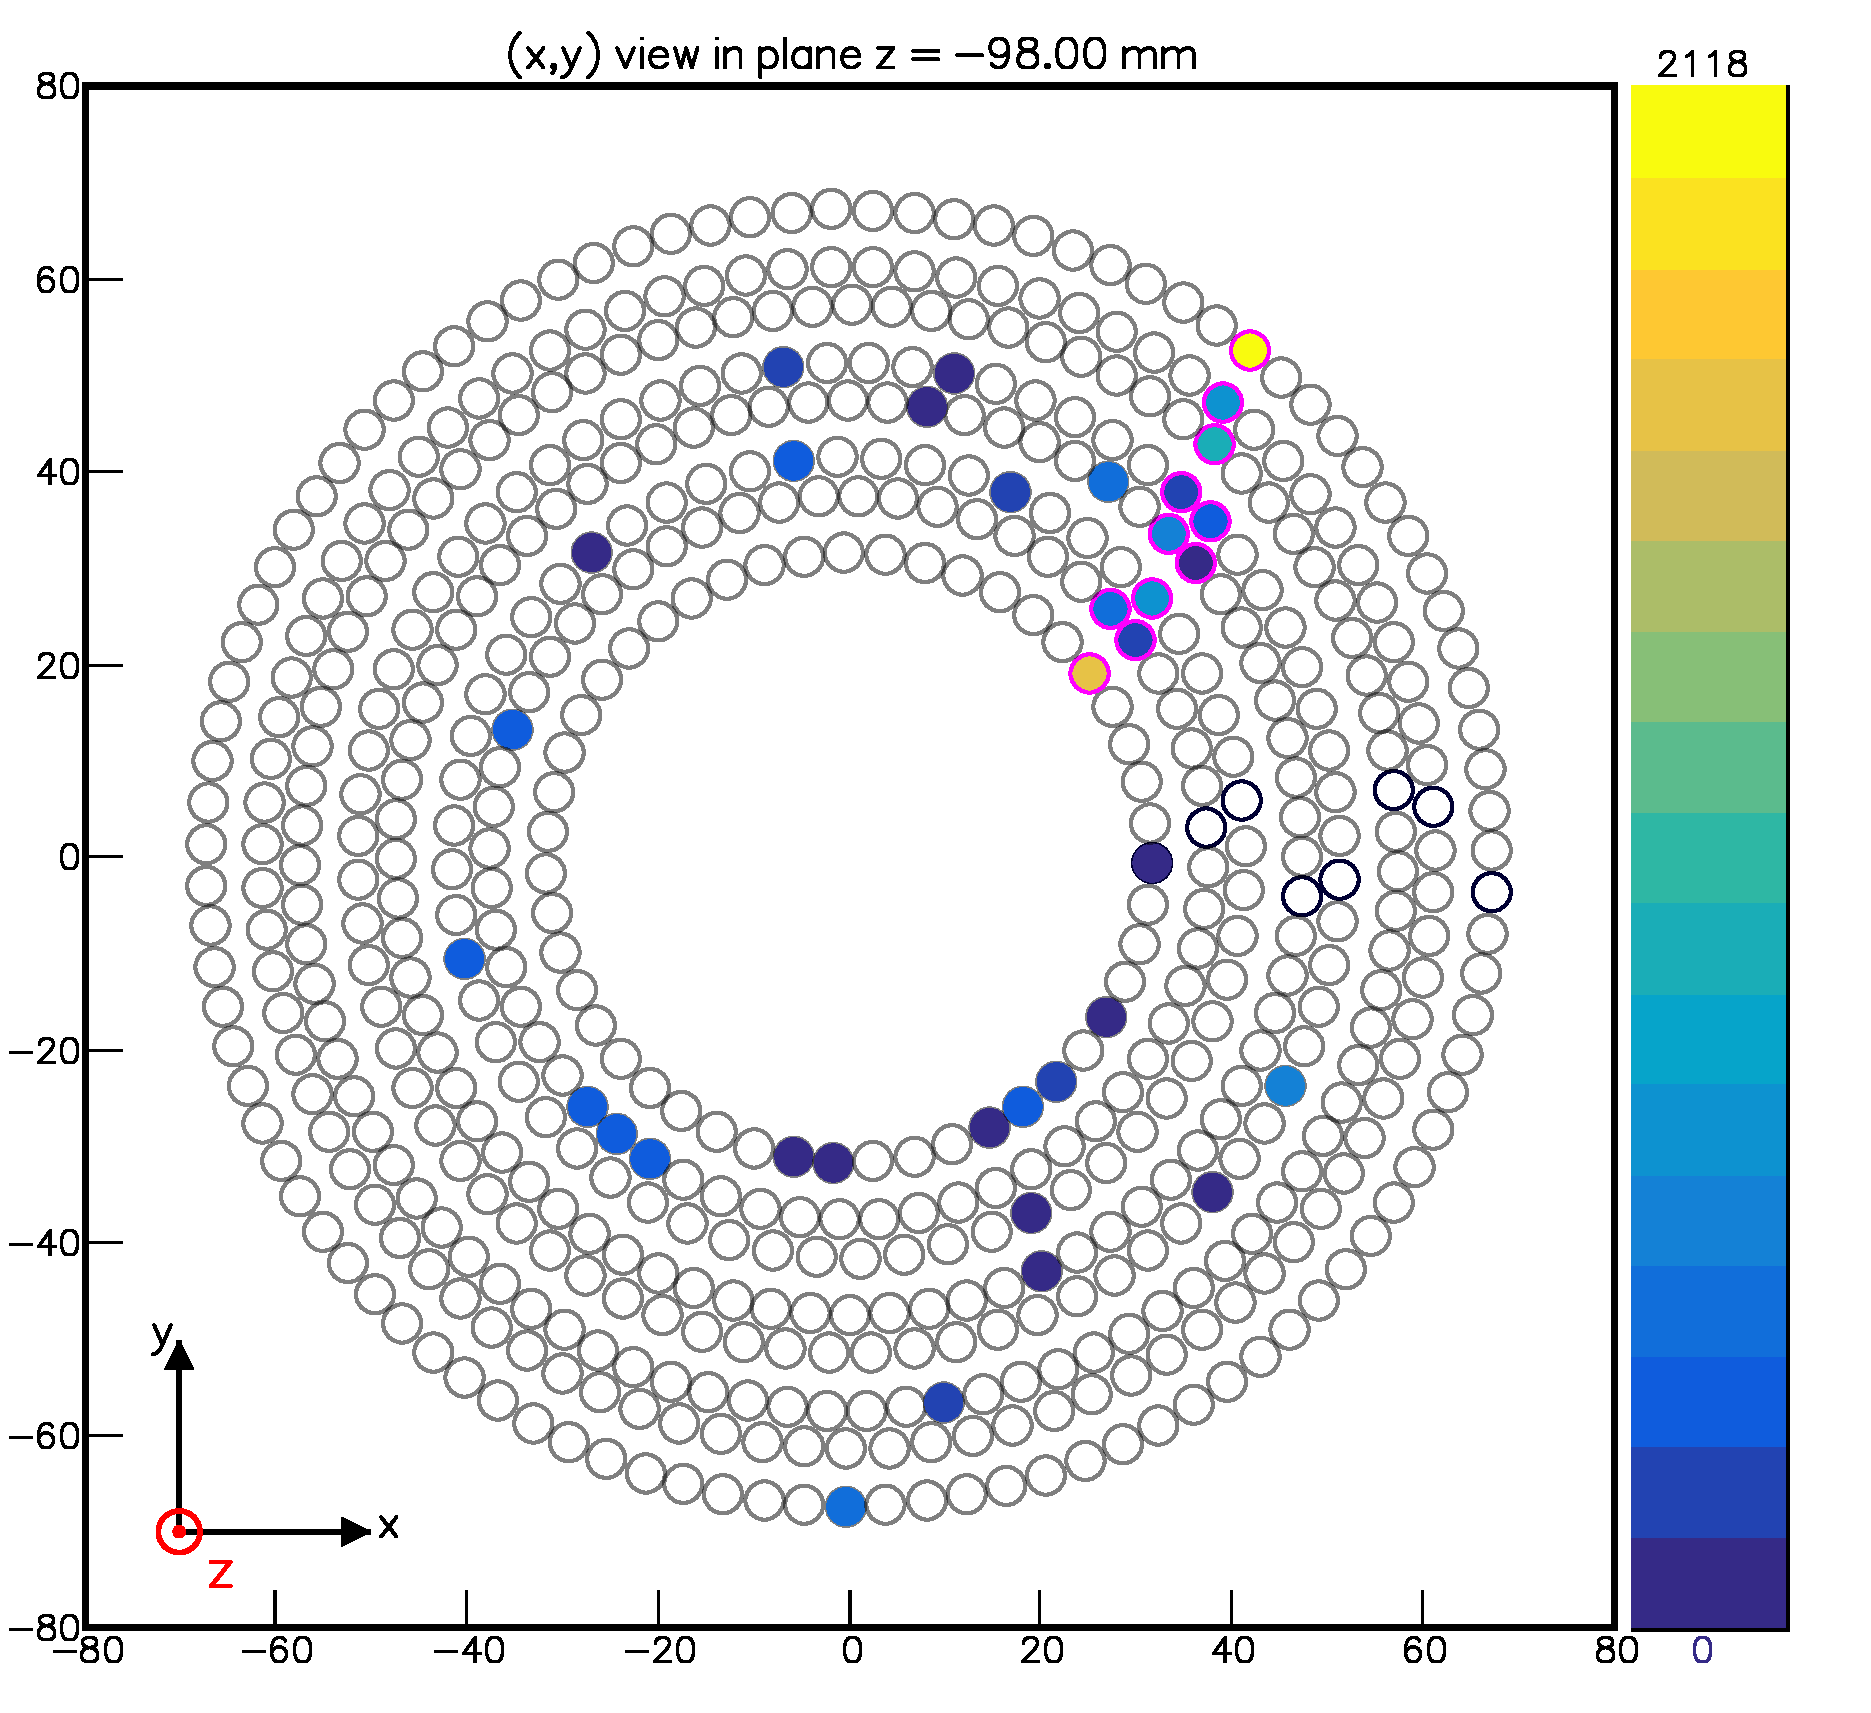
\includegraphics[width=0.45\linewidth]{figures/good_track_r22712_2gev_num_1.pdf} &
            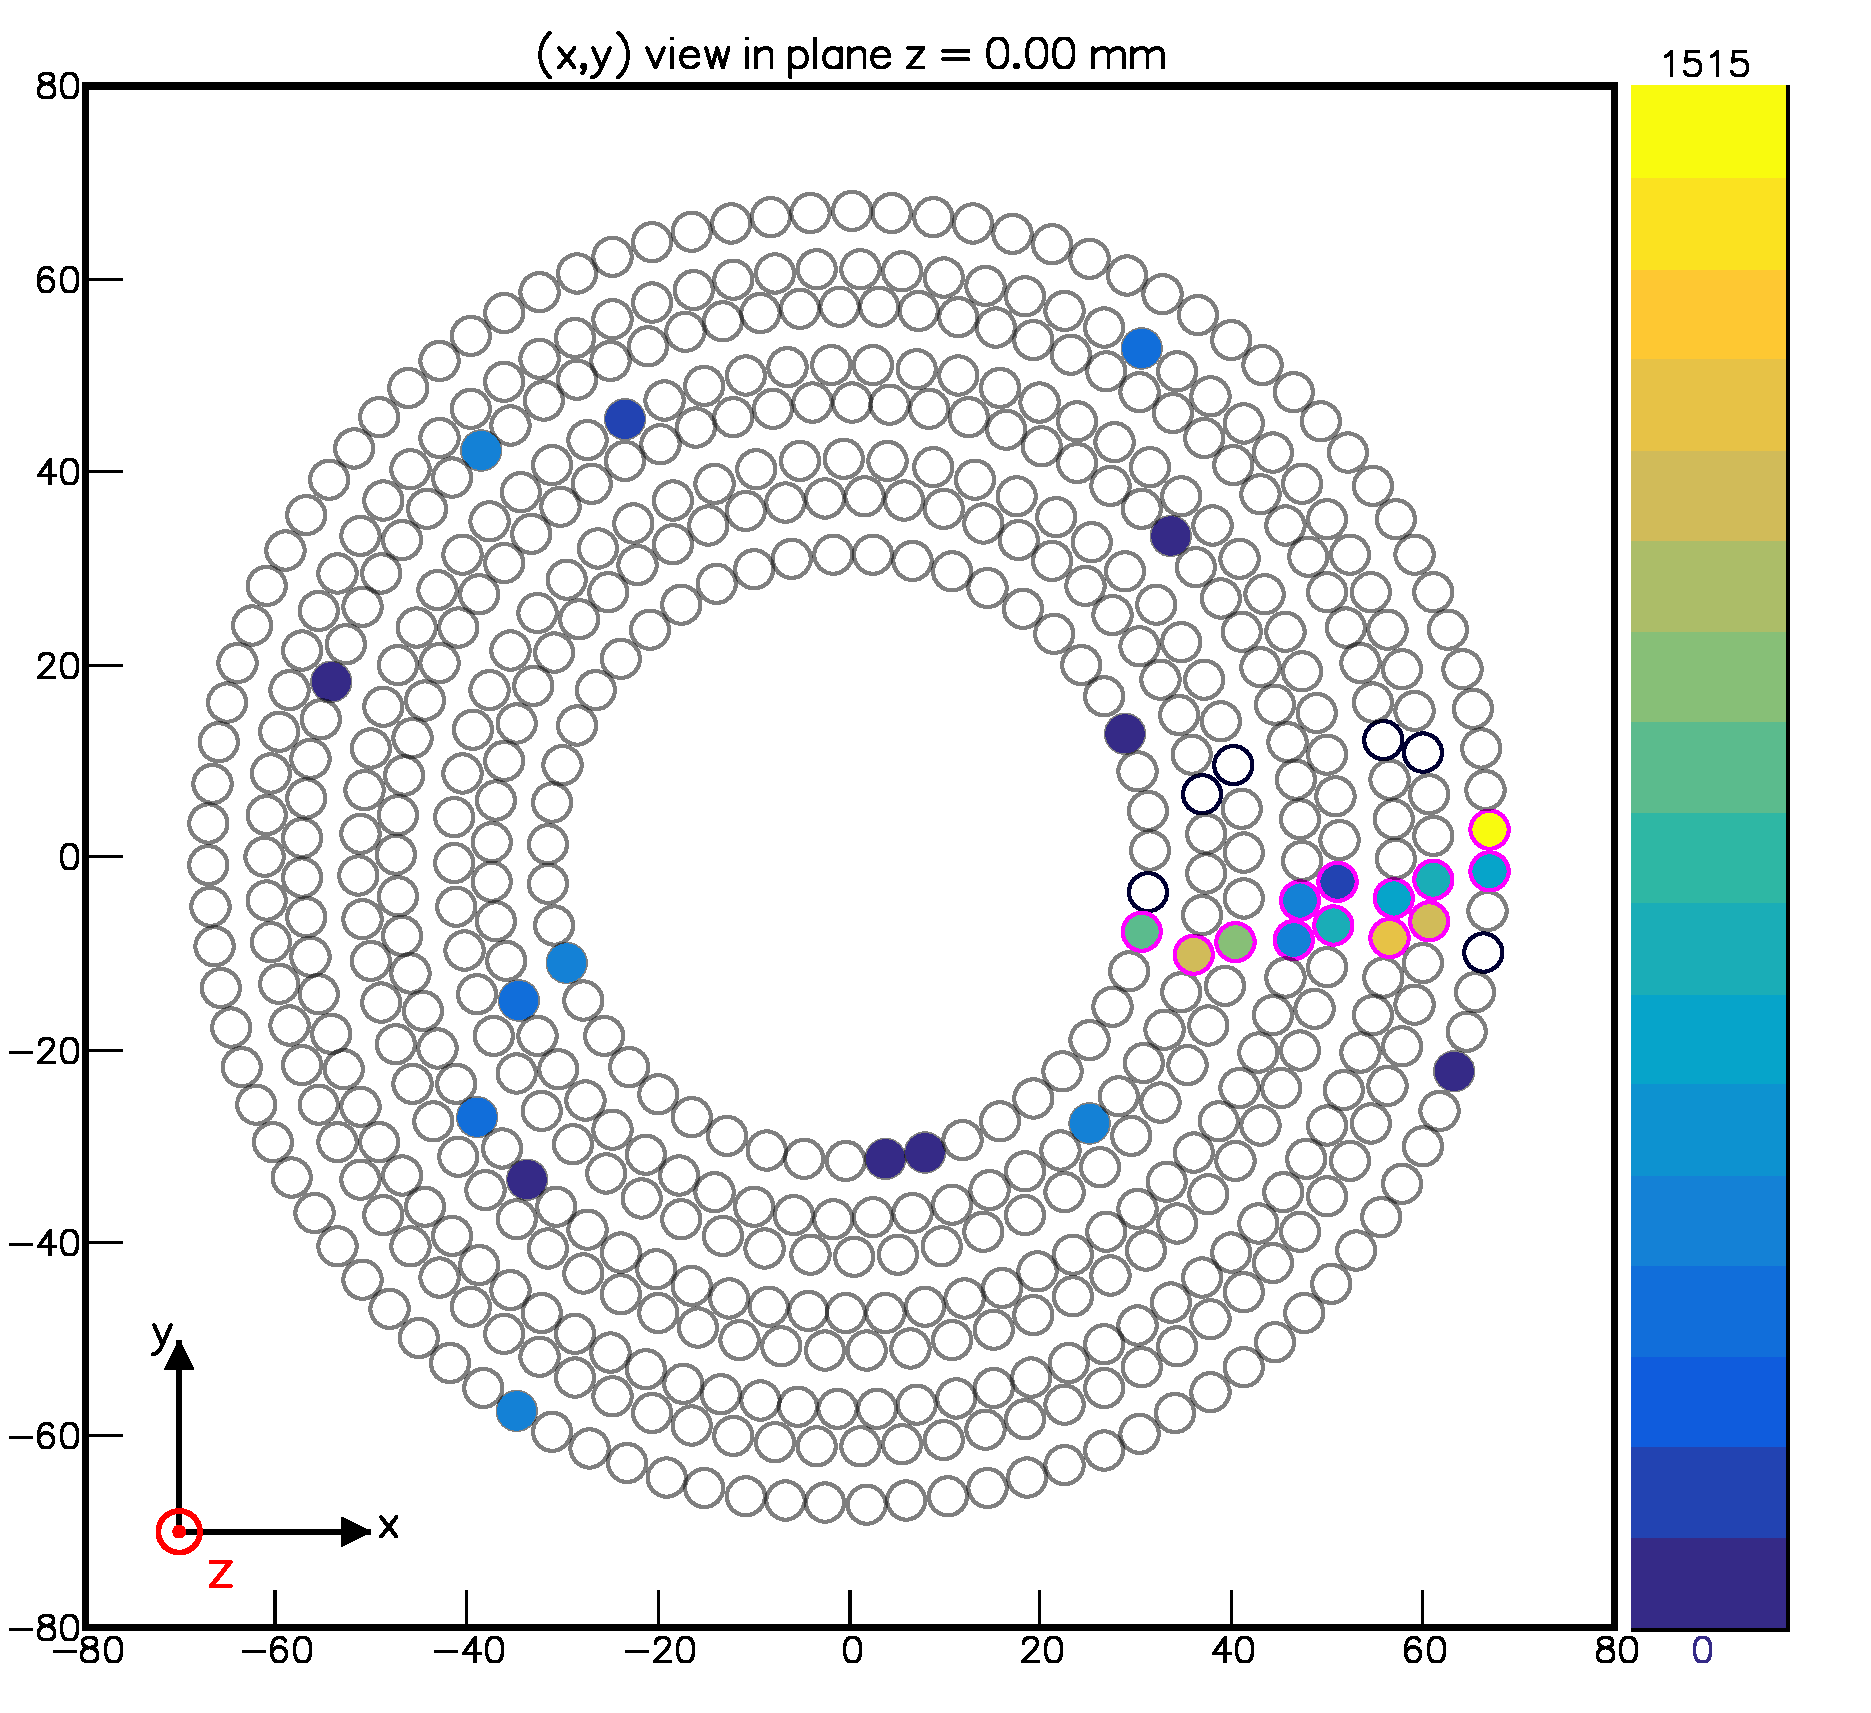
\includegraphics[width=0.45\linewidth]{figures/good_track_r22712_2gev_num_3.pdf}
    \end{tabular}


    \vfill

    {\footnotesize *All hits highlighted in magenta belongs to a reconstructed track}

\end{frame}


\begin{frame}{Issue with cut on the pedestal 1/2}
    \begin{itemize}
        \item Example of a good tracks with one missing hit
            \begin{itemize}
                \item The waveform of this missing hit is plotted on the right
                \item It pedestal does not pass the selection cut : $120 < \mbox{PED} < 350$
                \item Here the pedestal is 500.25 ADC
            \end{itemize}
        \item 
        
        
    \end{itemize}

    \centering
    \vspace{0.2cm}

    \begin{tabular}{cc}
        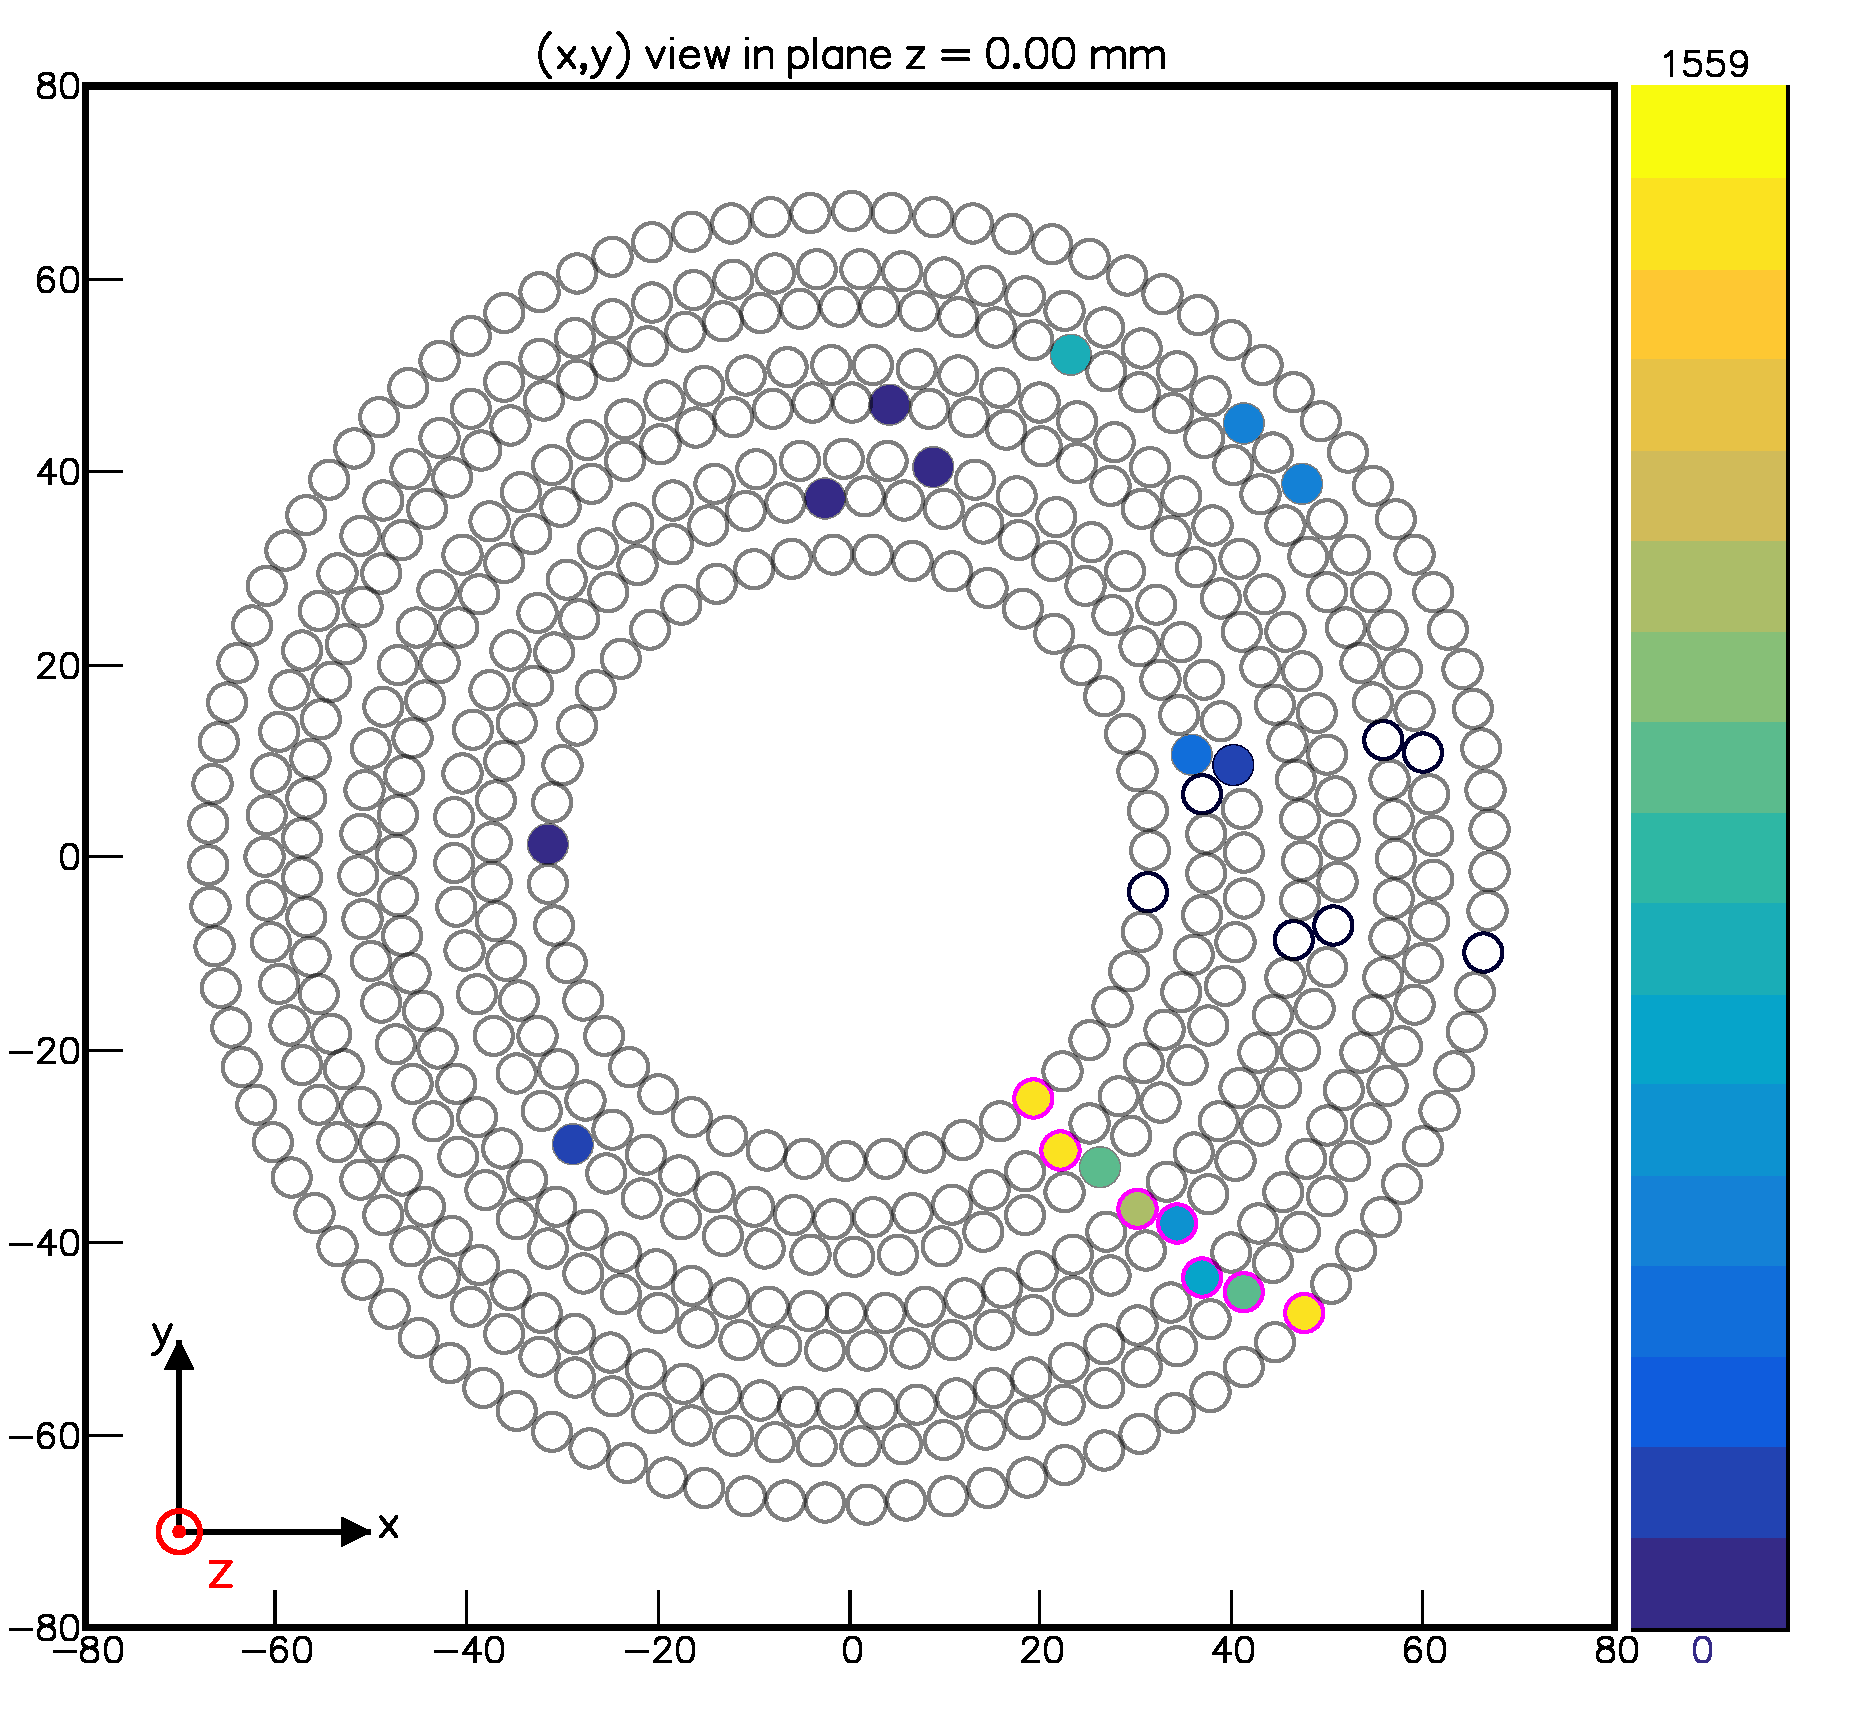
\includegraphics[width=0.45\linewidth]{figures/good_track_r22712_2gev_num_2_one_missing_hit_due_to_bad_ped.pdf} &
            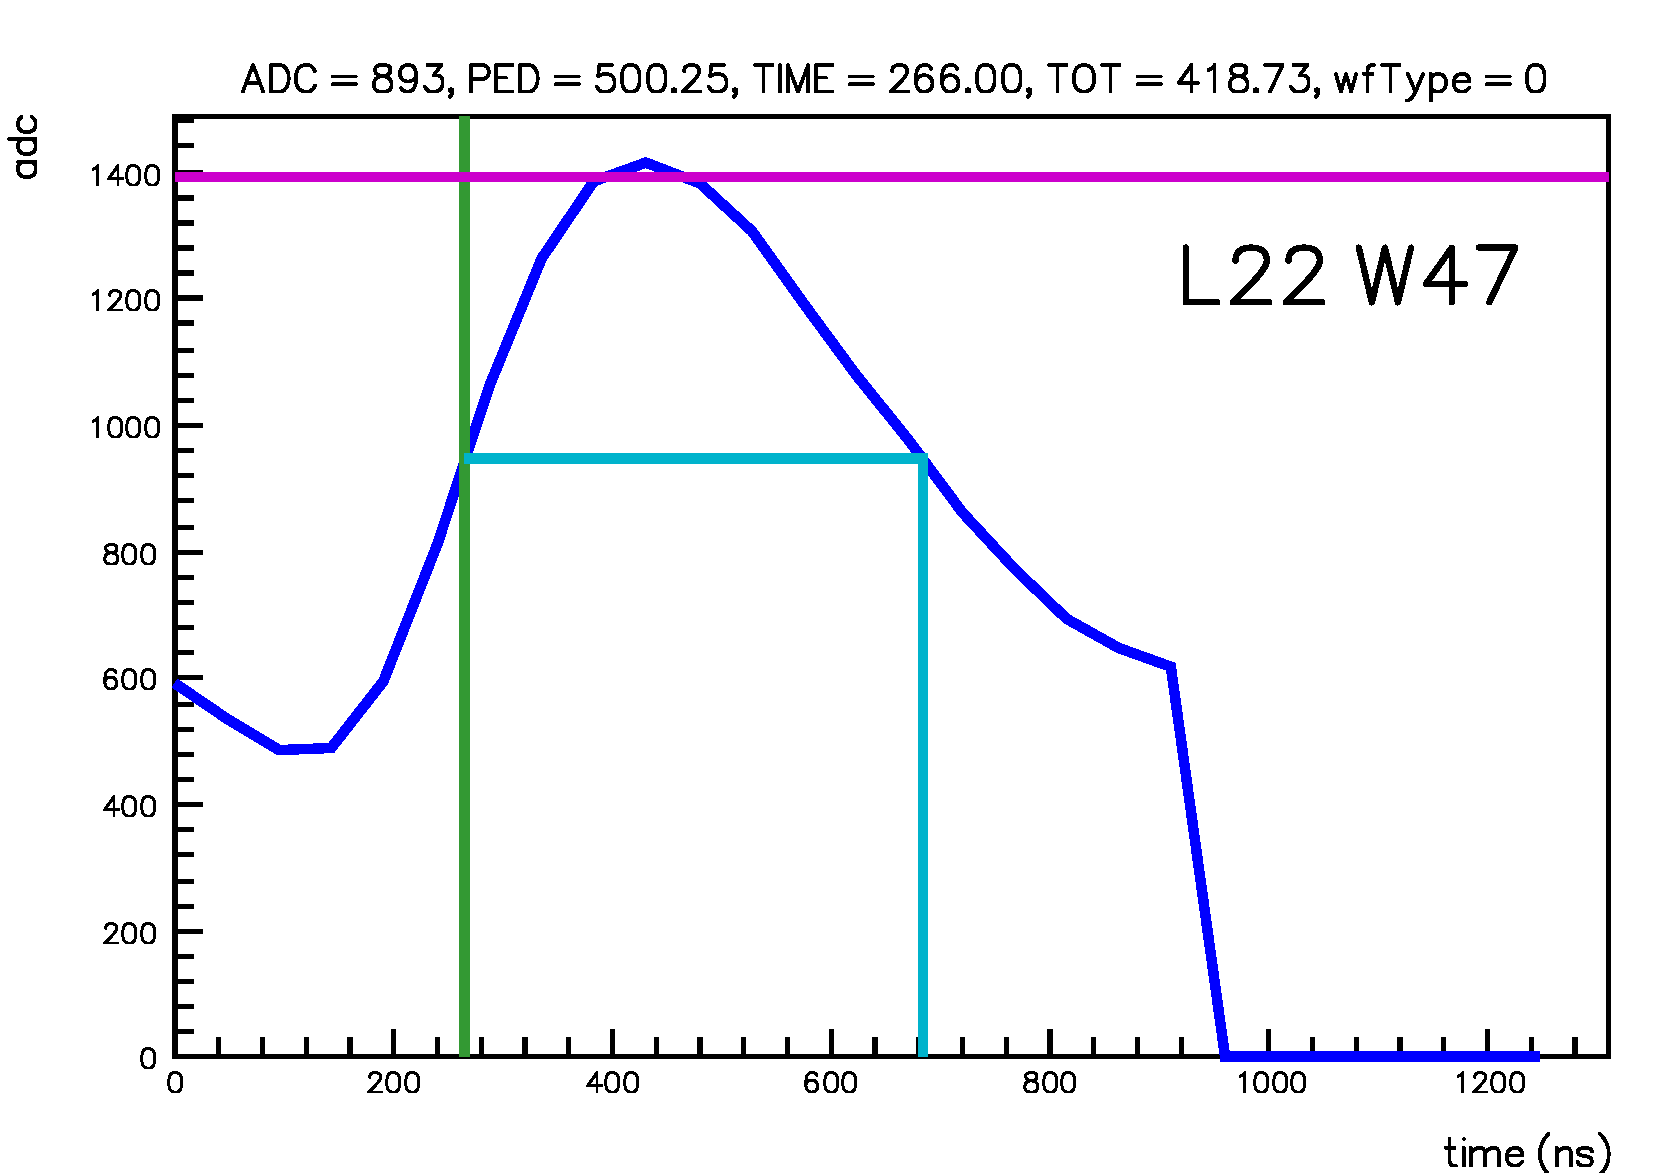
\includegraphics[width=0.45\linewidth]{figures/good_track_r22712_2gev_num_2_one_missing_hit_due_to_bad_ped_wf.pdf}
    \end{tabular}

\end{frame}

\begin{frame}{Issue with cut on the pedestal 2/2}
    \begin{itemize}
        \item Example of a potential good tracks not reconstructed due to the bad pedestal
            \begin{itemize}
                \item Here all pedestals are above 350 ADC, so no hits were selected
                \item Typical the signal in L11W25 is good, even if the baseline is around 1000 ADC
                \item Reminder: during data acquisition, in mode TPC, we only kept, samples above threshold + few before and after (see appendix, last slide)
                \item I think to remove the cut the pedestal
            \end{itemize}
        
        
    \end{itemize}

    \centering
    \vspace{0.2cm}

    \begin{minipage}{0.4\textwidth}
        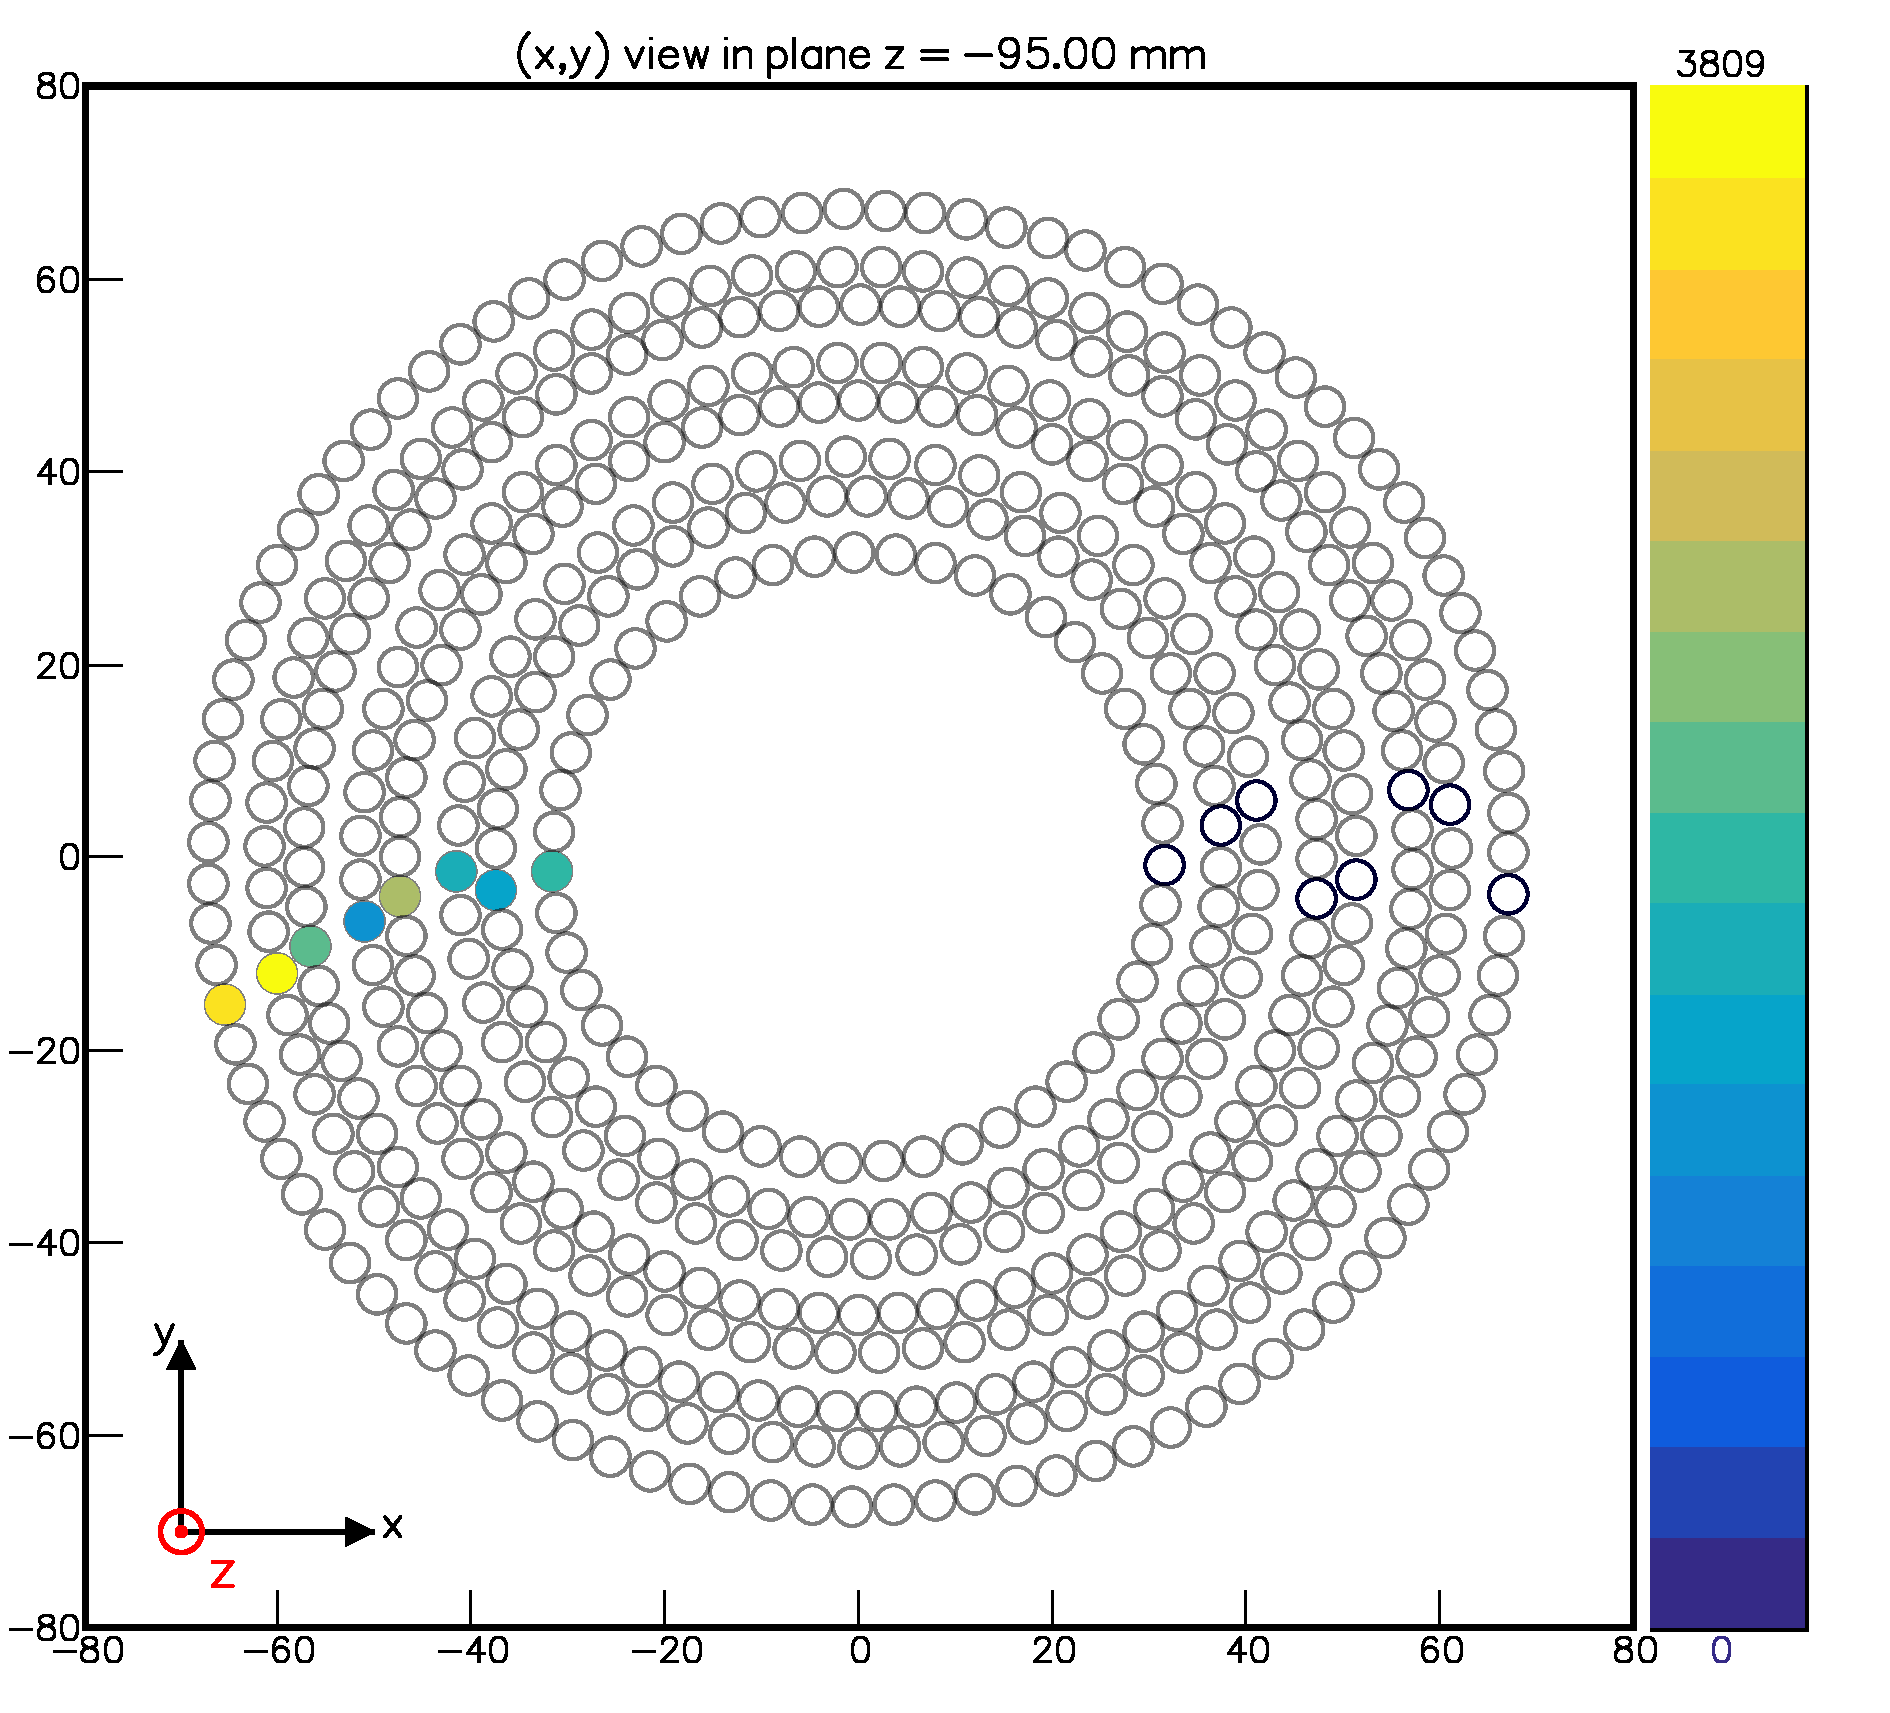
\includegraphics[width=\linewidth]{figures/good_track_not_reconstructed_due_to_bad_pedestal.pdf}
    \end{minipage}
    \begin{minipage}{0.58\textwidth}
        \begin{tabular}{cc}
            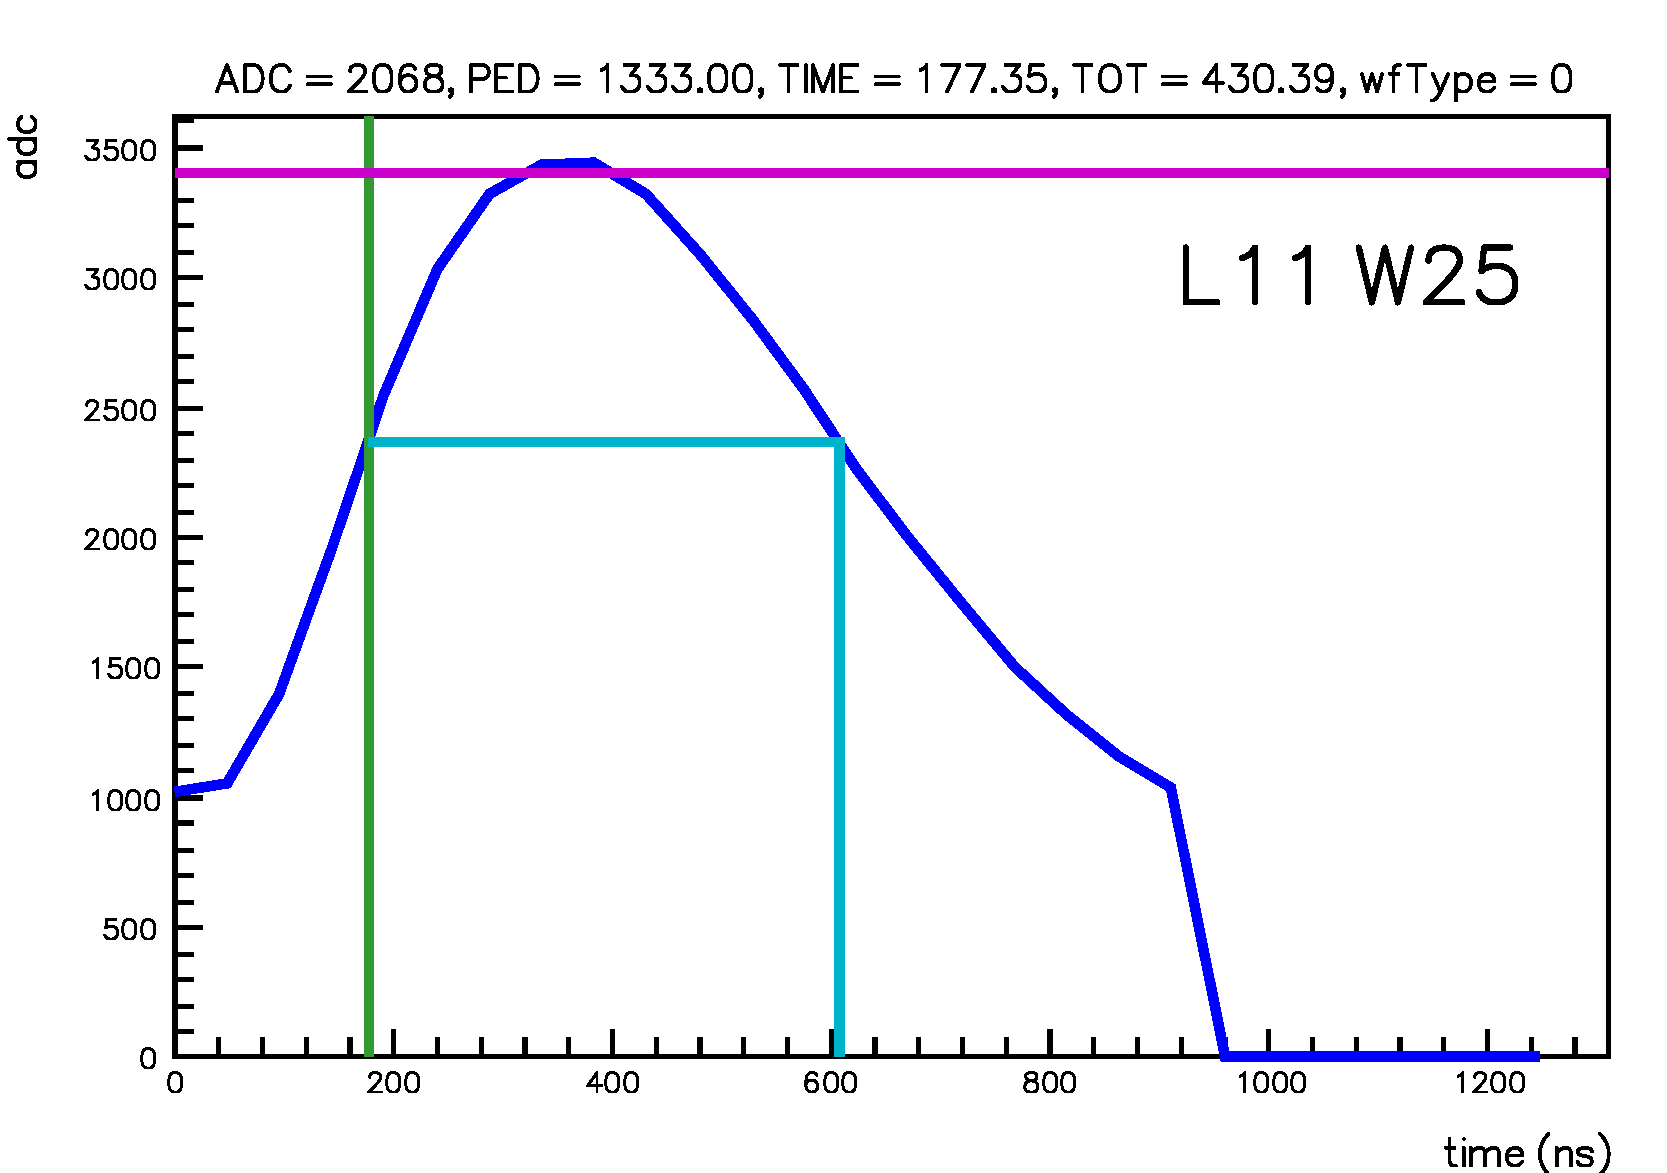
\includegraphics[width=0.45\textwidth]{figures/good_track_not_reconstructed_due_to_bad_pedestal_wf1.pdf} &
                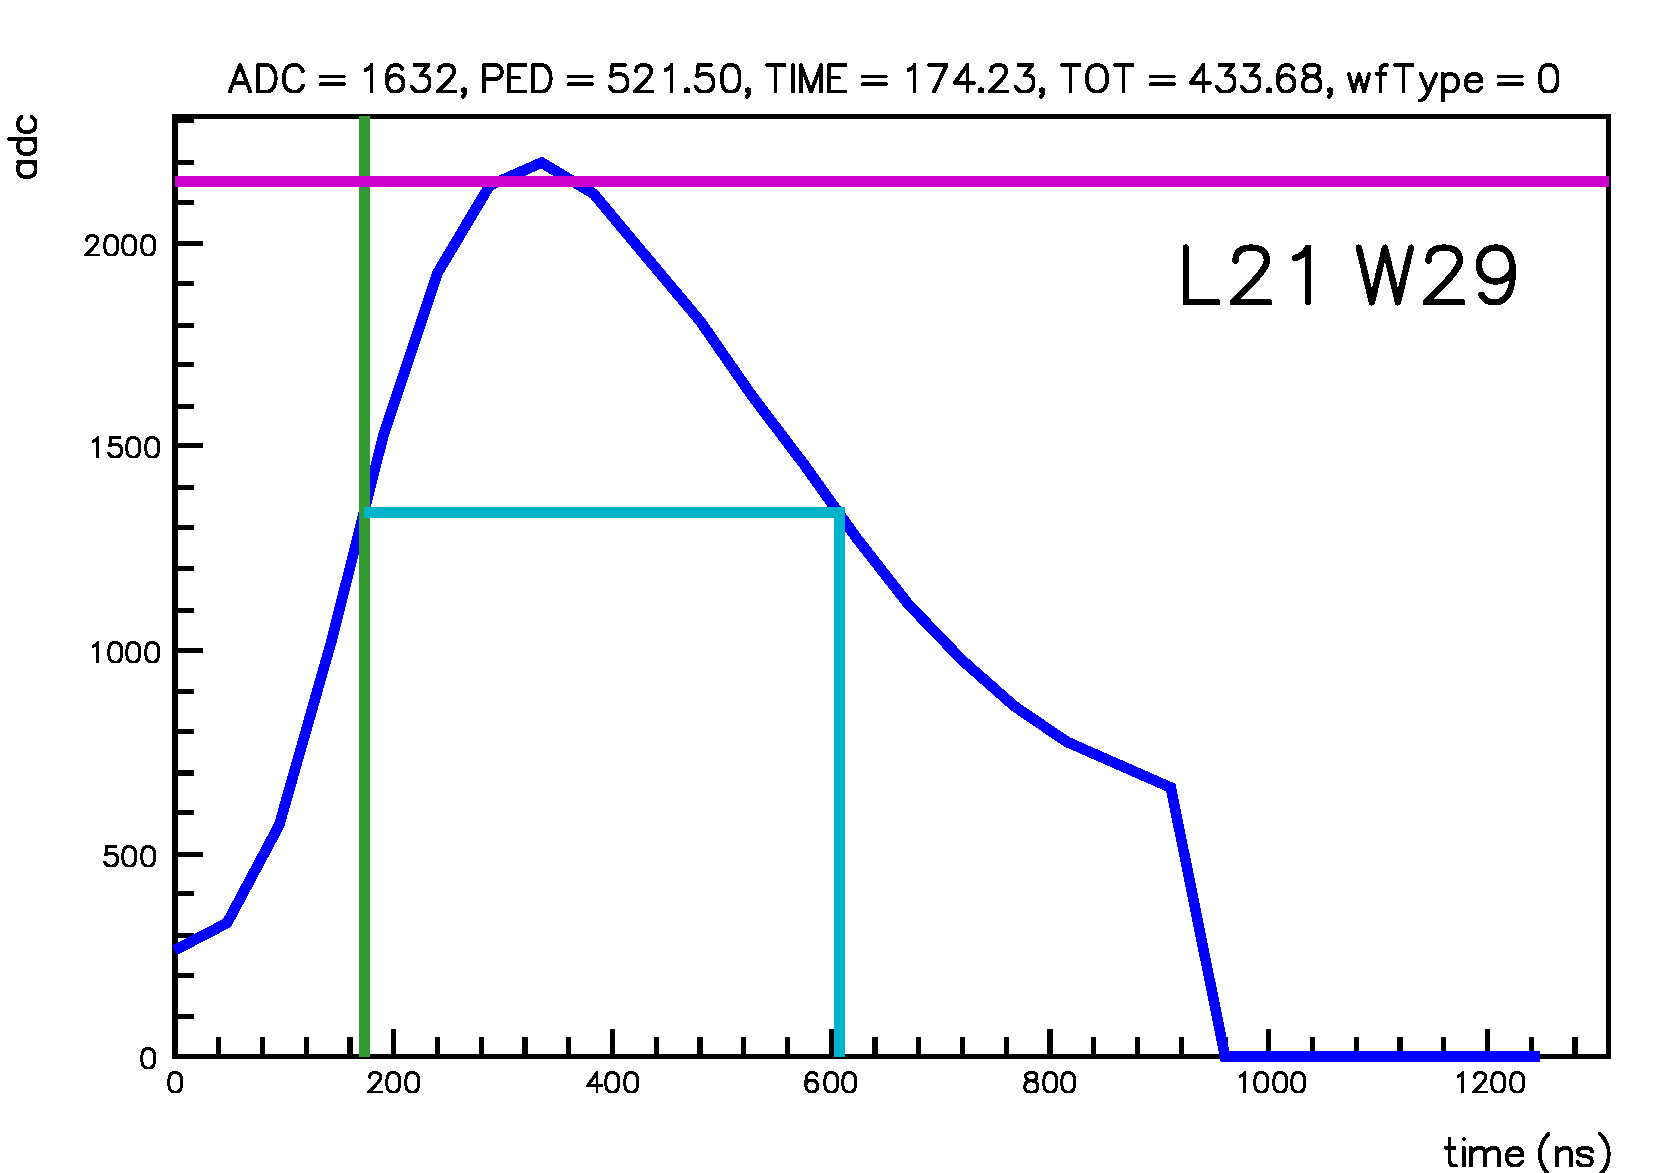
\includegraphics[width=0.45\textwidth]{figures/good_track_not_reconstructed_due_to_bad_pedestal_wf2.pdf} \\
            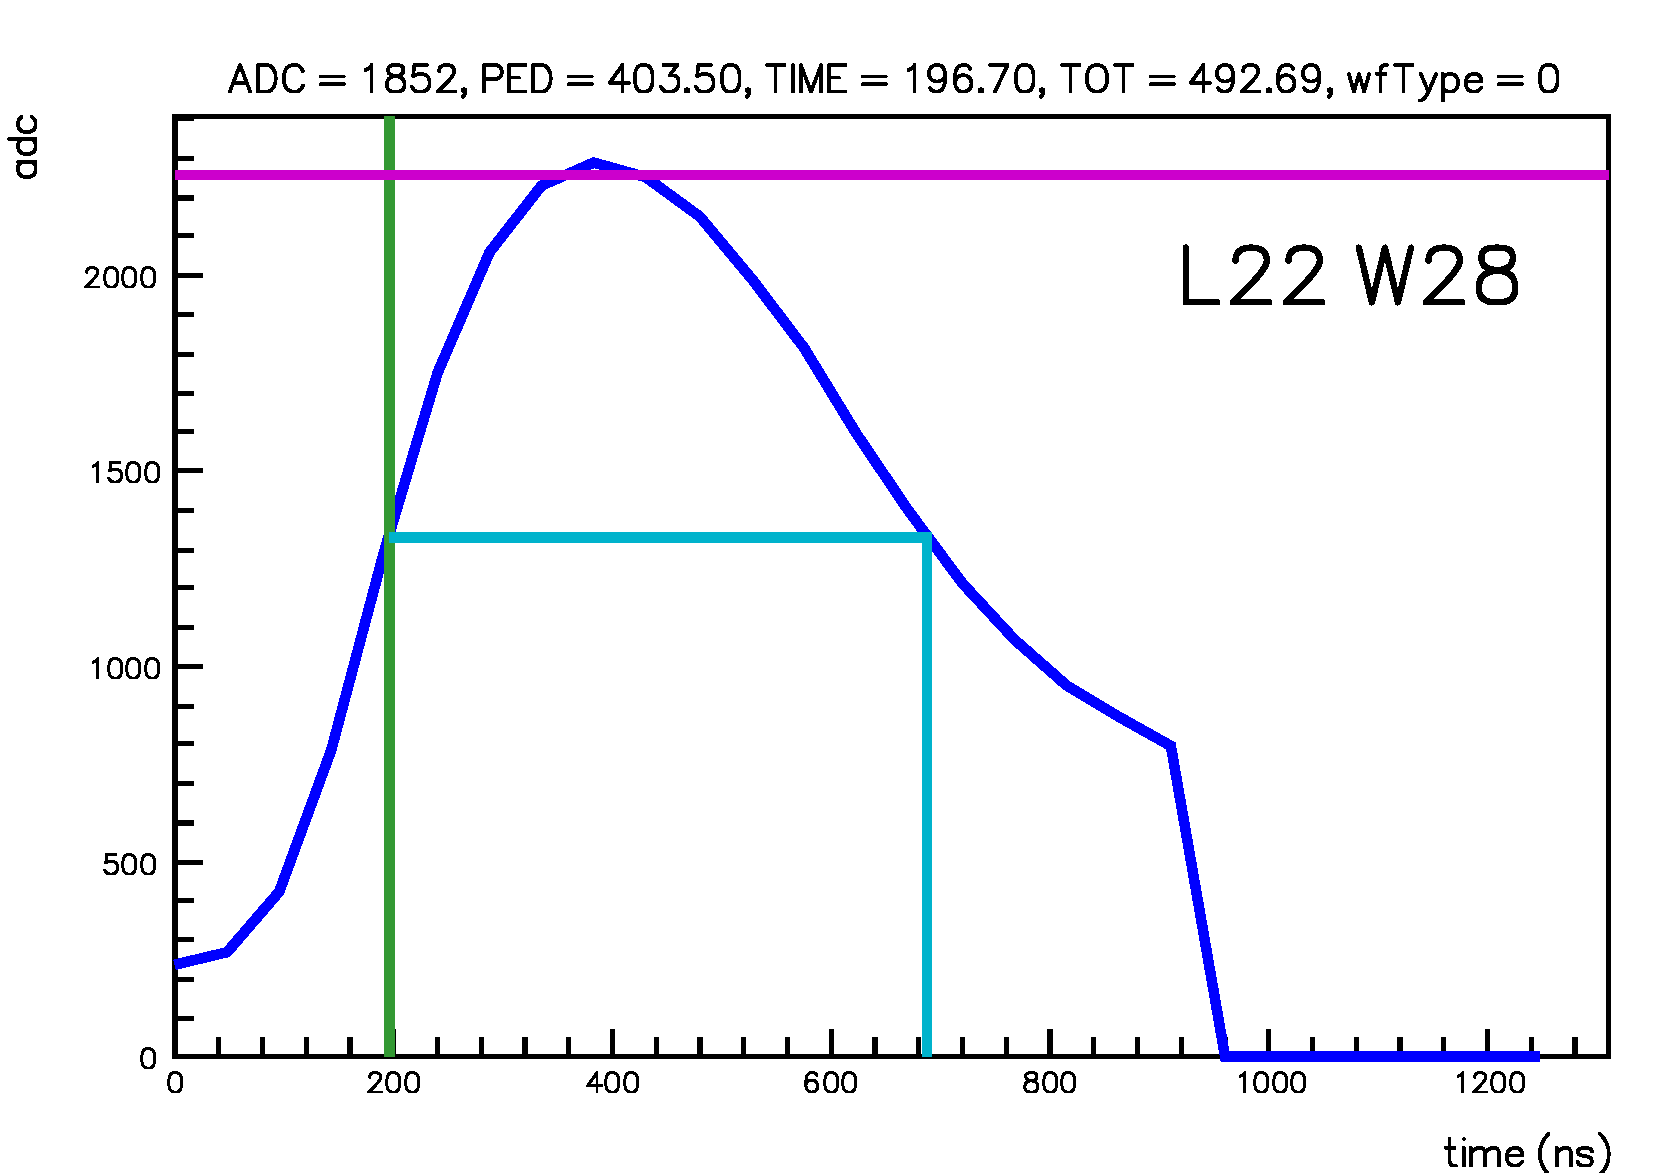
\includegraphics[width=0.45\textwidth]{figures/good_track_not_reconstructed_due_to_bad_pedestal_wf3.pdf} &
                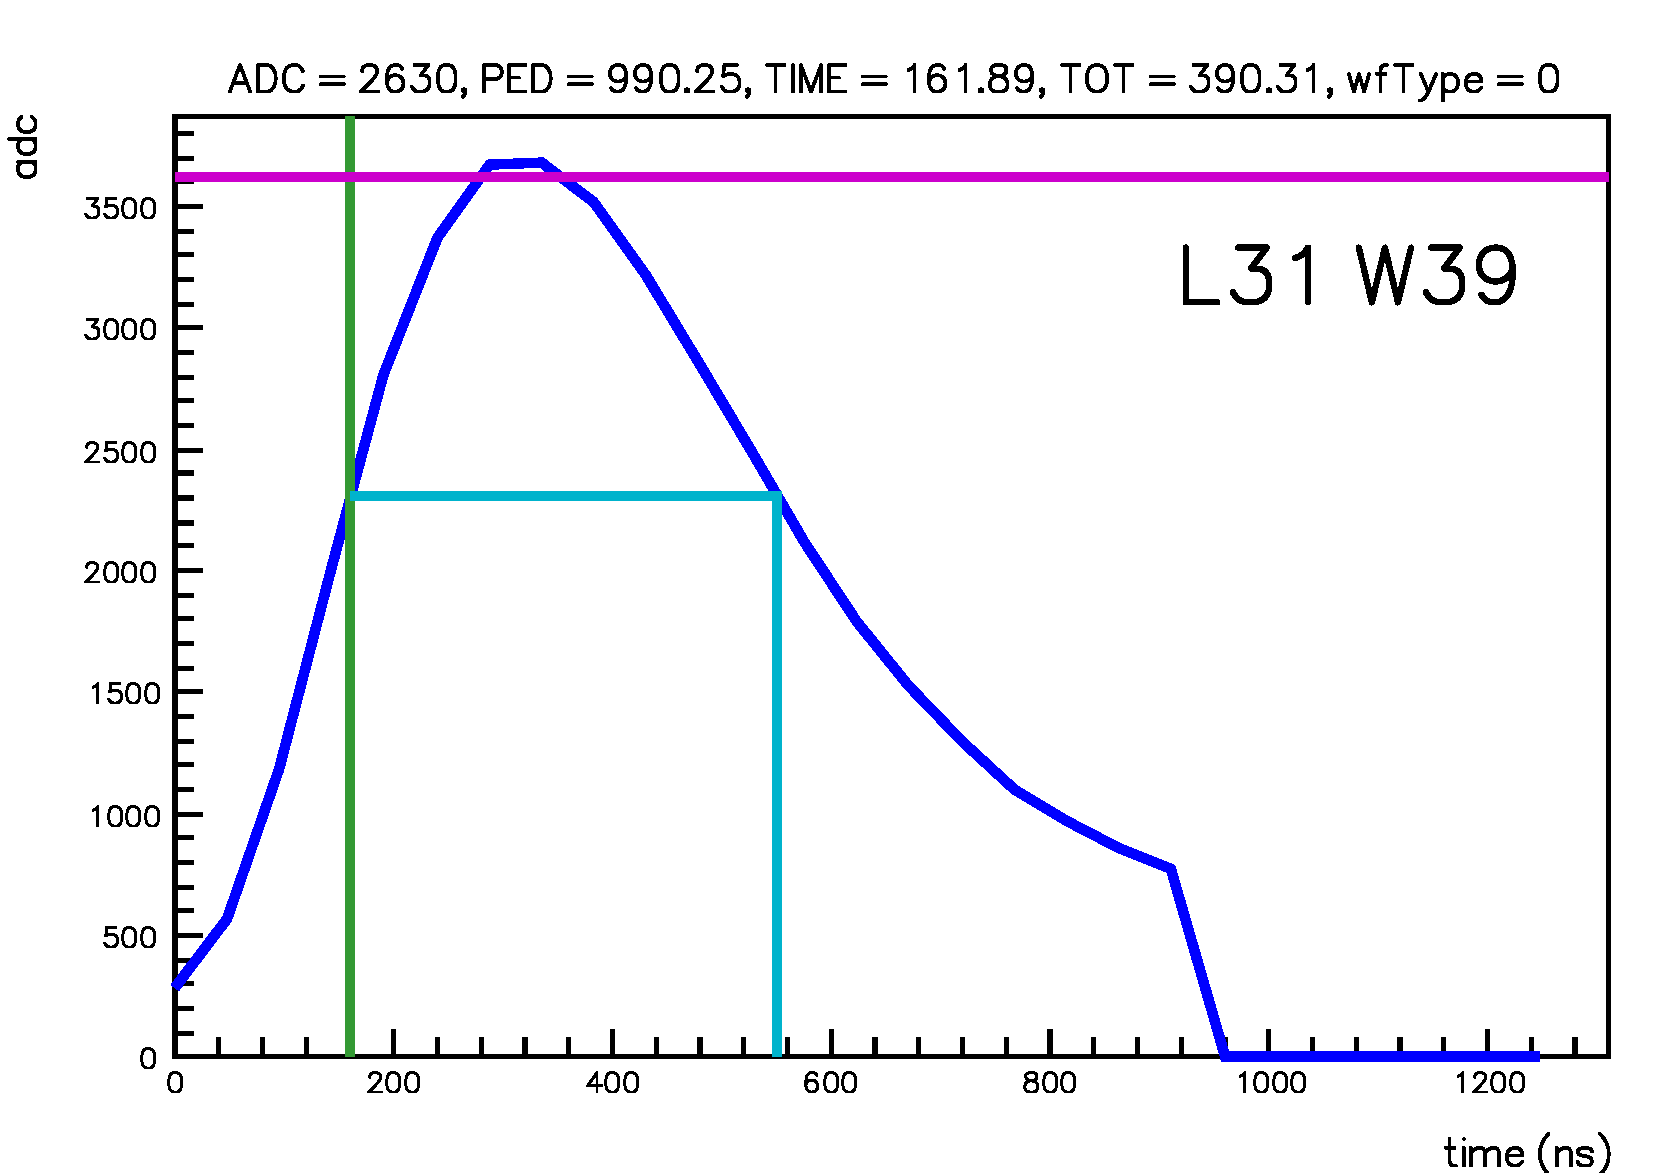
\includegraphics[width=0.45\textwidth]{figures/good_track_not_reconstructed_due_to_bad_pedestal_wf4.pdf} \\
        \end{tabular}
    \end{minipage}

    % \begin{tabular}{cc}
    %     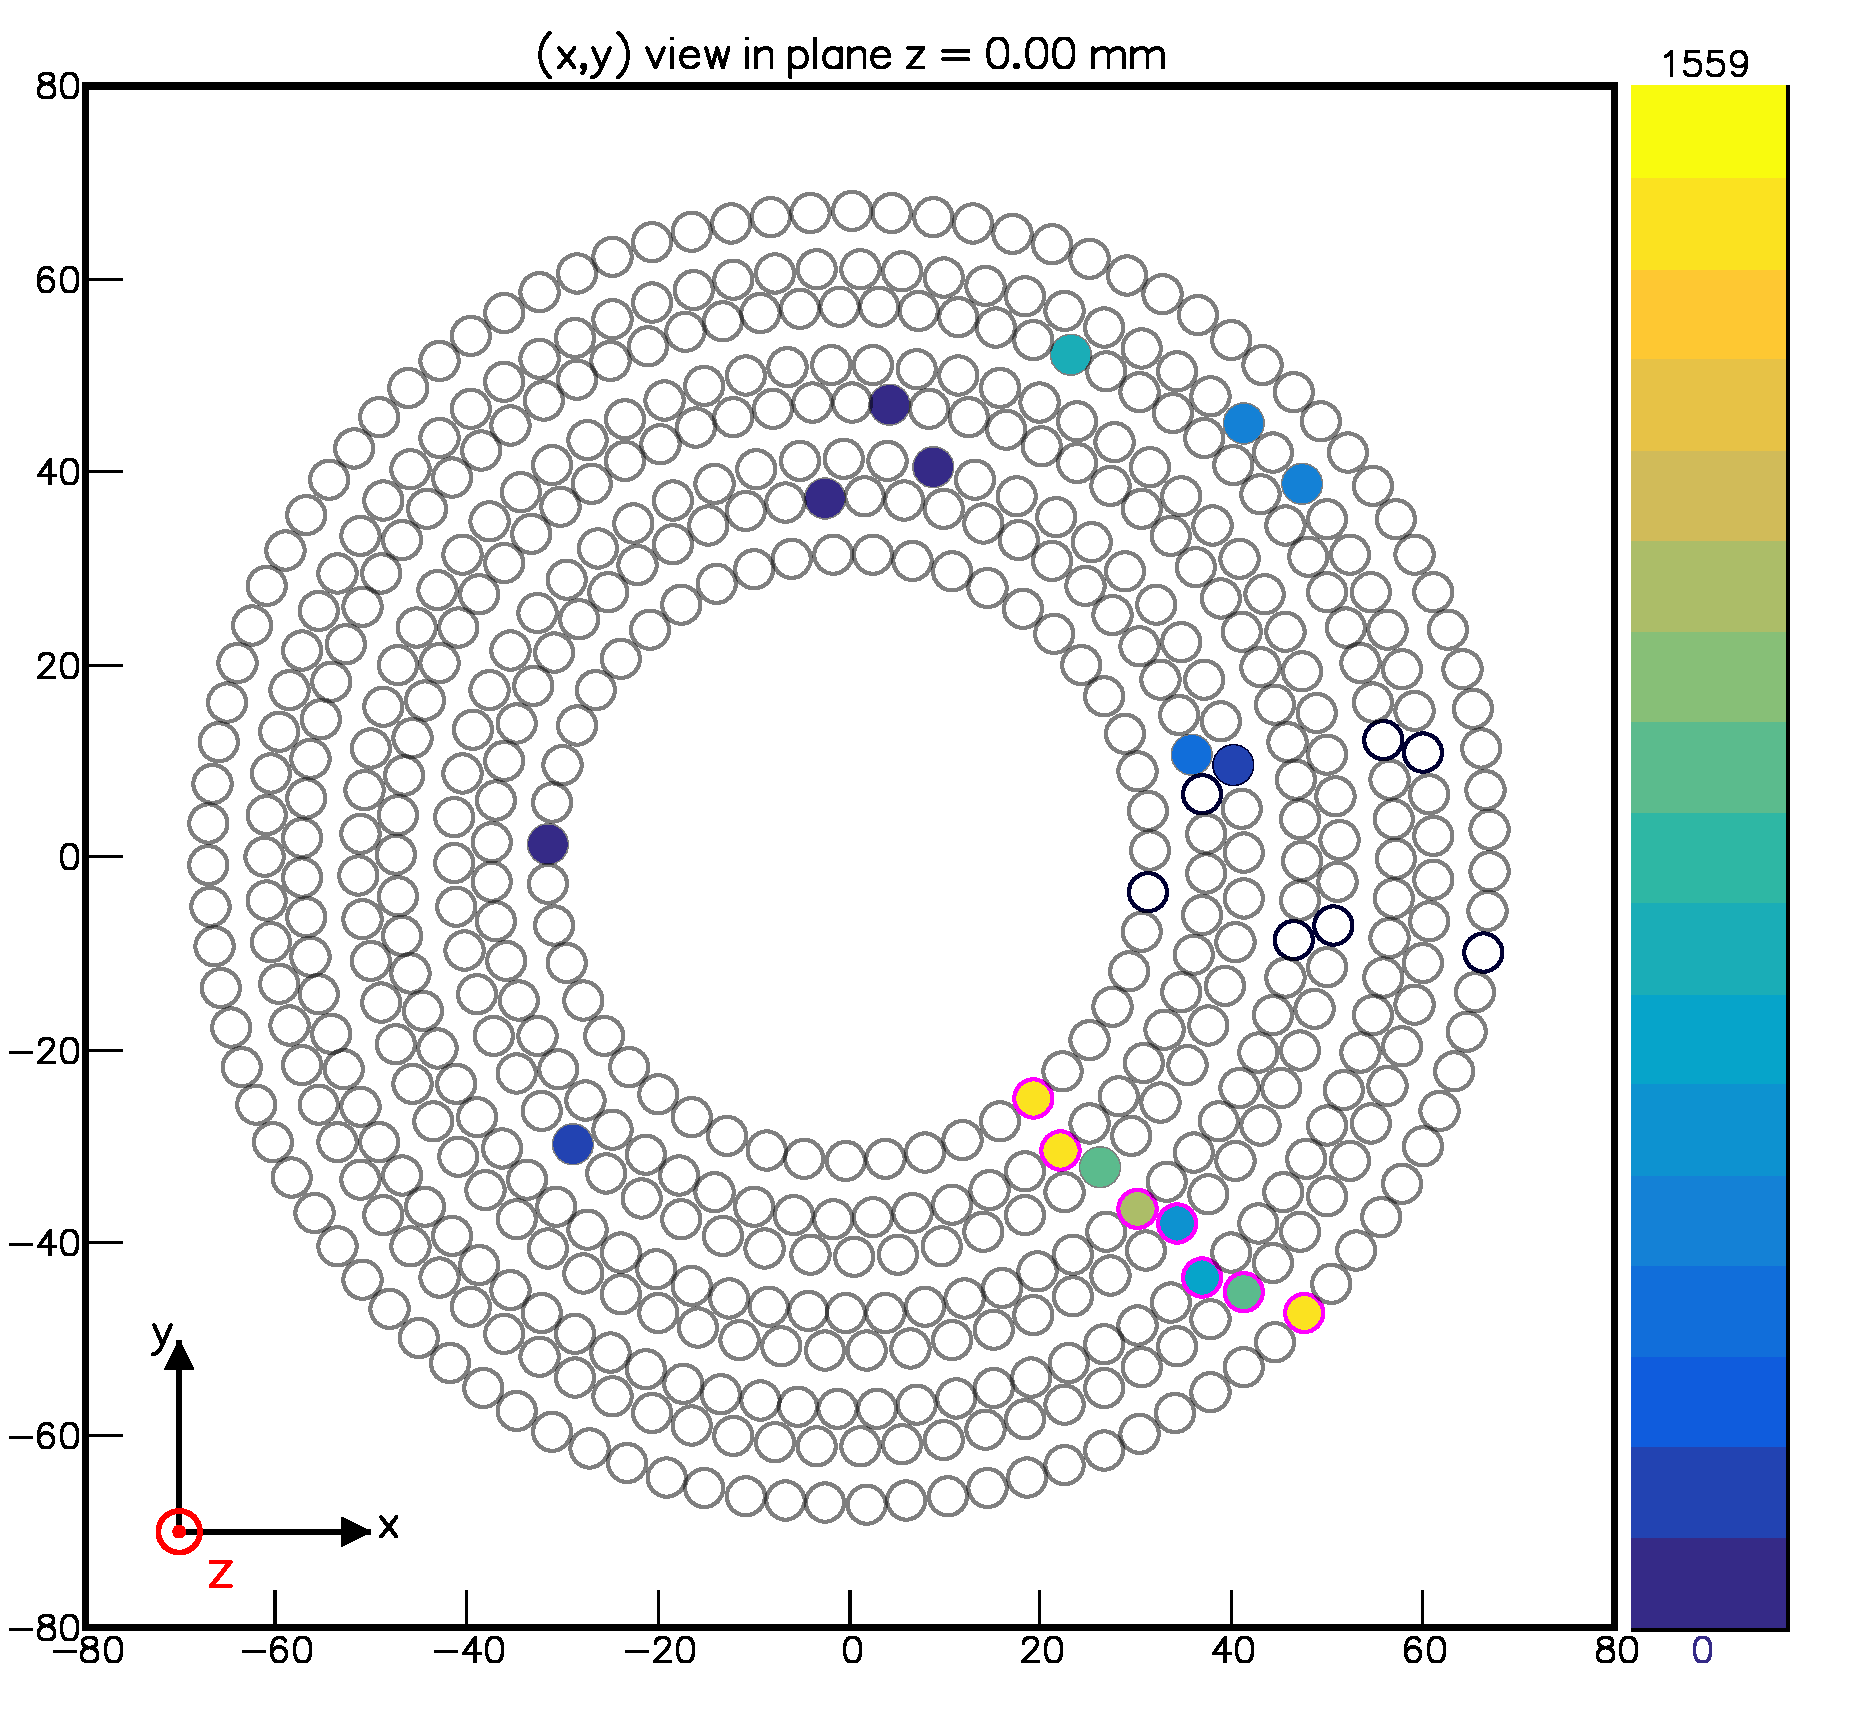
\includegraphics[width=0.45\linewidth]{figures/good_track_r22712_2gev_num_2_one_missing_hit_due_to_bad_ped.pdf} &
    %         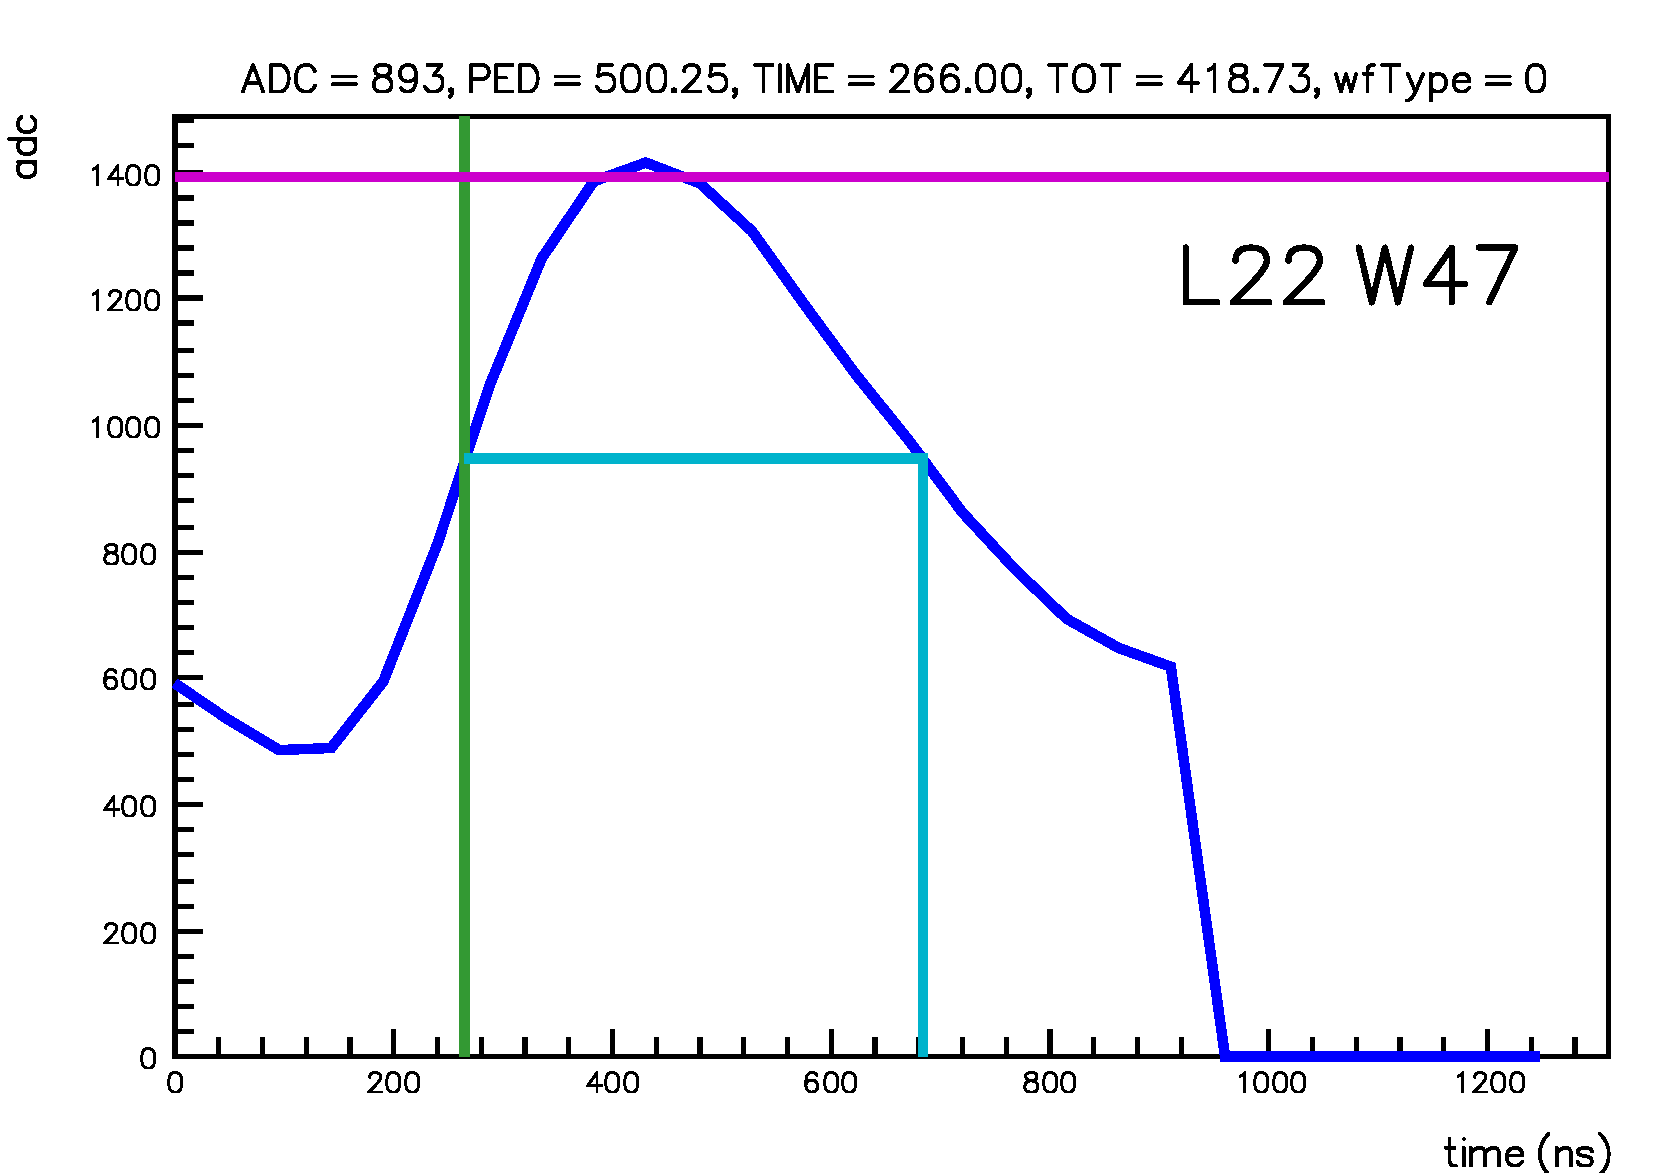
\includegraphics[width=0.45\linewidth]{figures/good_track_r22712_2gev_num_2_one_missing_hit_due_to_bad_ped_wf.pdf}
    % \end{tabular}

\end{frame}


\begin{frame}{Issue with cut on the time over threshold}
    \begin{itemize}
        \item I don't have much issue with the ToT, but I think to reduce the lower limit at 250 ns due to the apparent cut at 300 ns
        
            \begin{itemize}
                \item In the example, the hits on layer 42 and 51 are missing
                \item The hit on layer 42 has $\mbox{ToT} < 300$ ns, so not selected
                \item The hit on layer 51, has certainly been excluded in the second pass of the Kalman Filter by having a residual much bigger than 1.5 mm
            \end{itemize}
        
    \end{itemize}

    \centering
    \vspace{0.2cm}

    \begin{minipage}{0.58\textwidth}
        \centering
        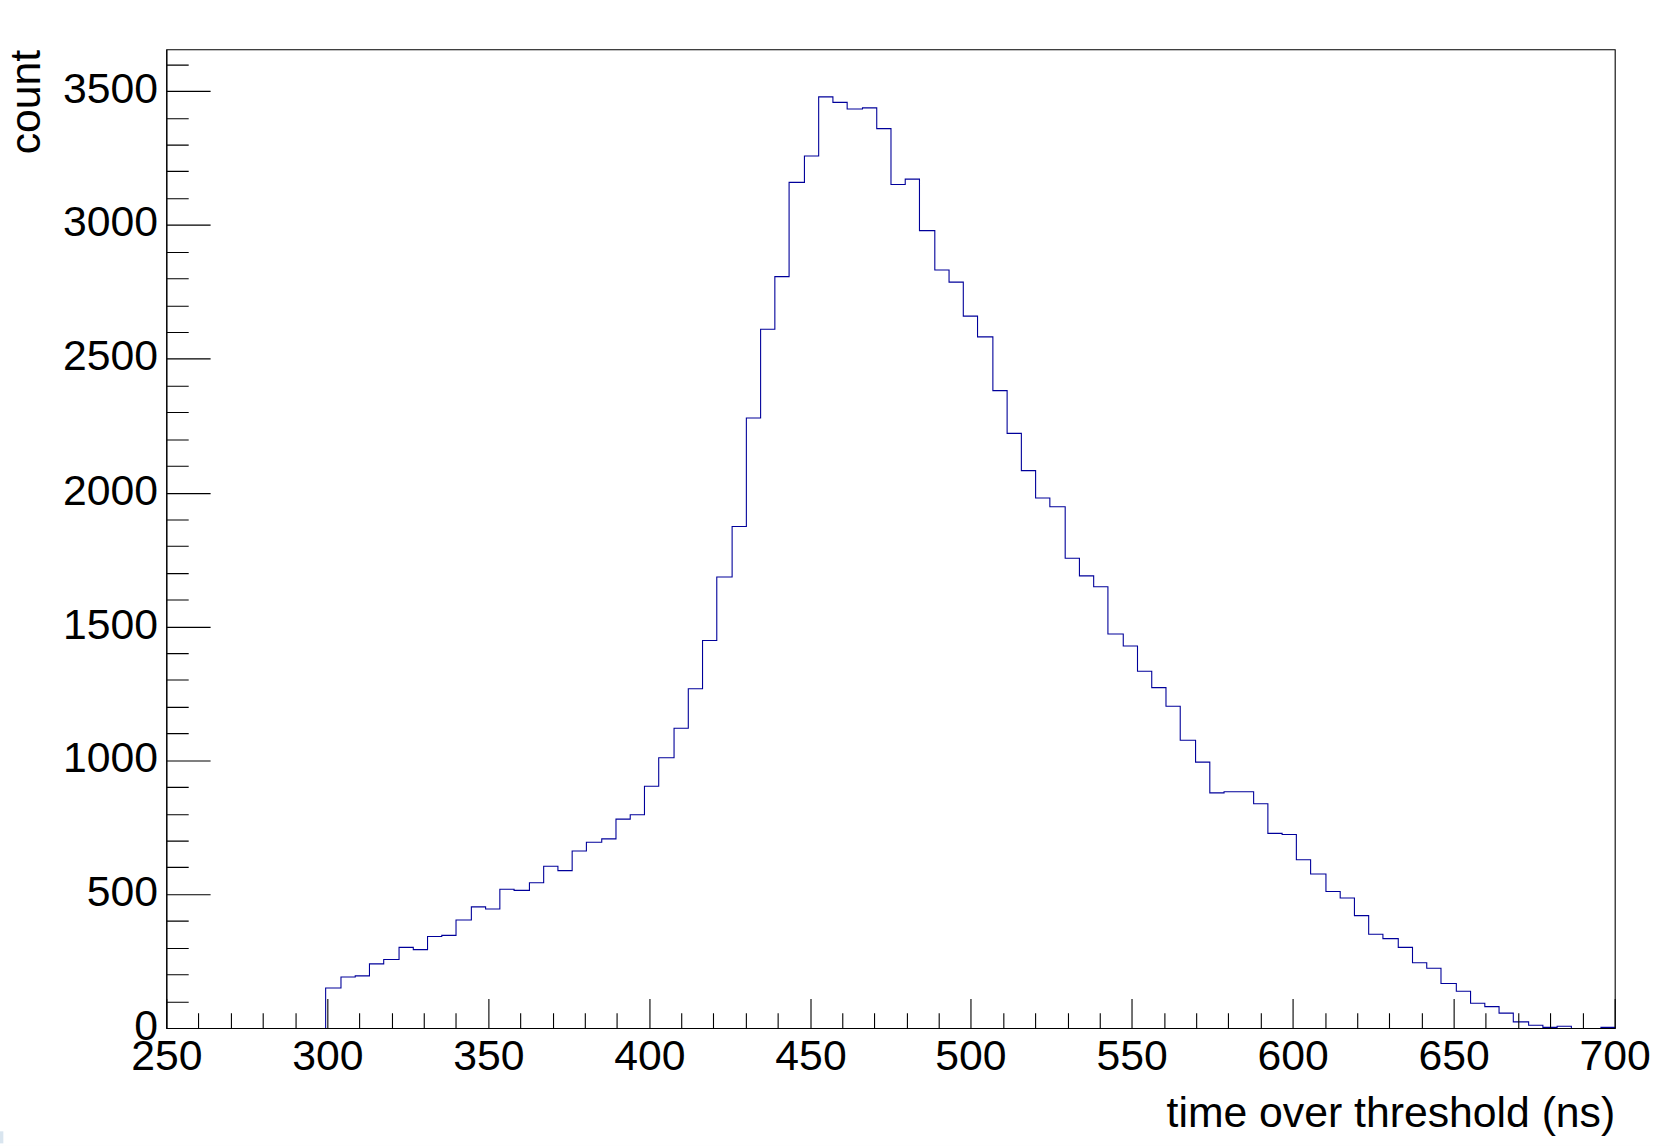
\includegraphics[width=0.5\linewidth]{figures/timeOverThreshold.png}

        \begin{tabular}{cc}
            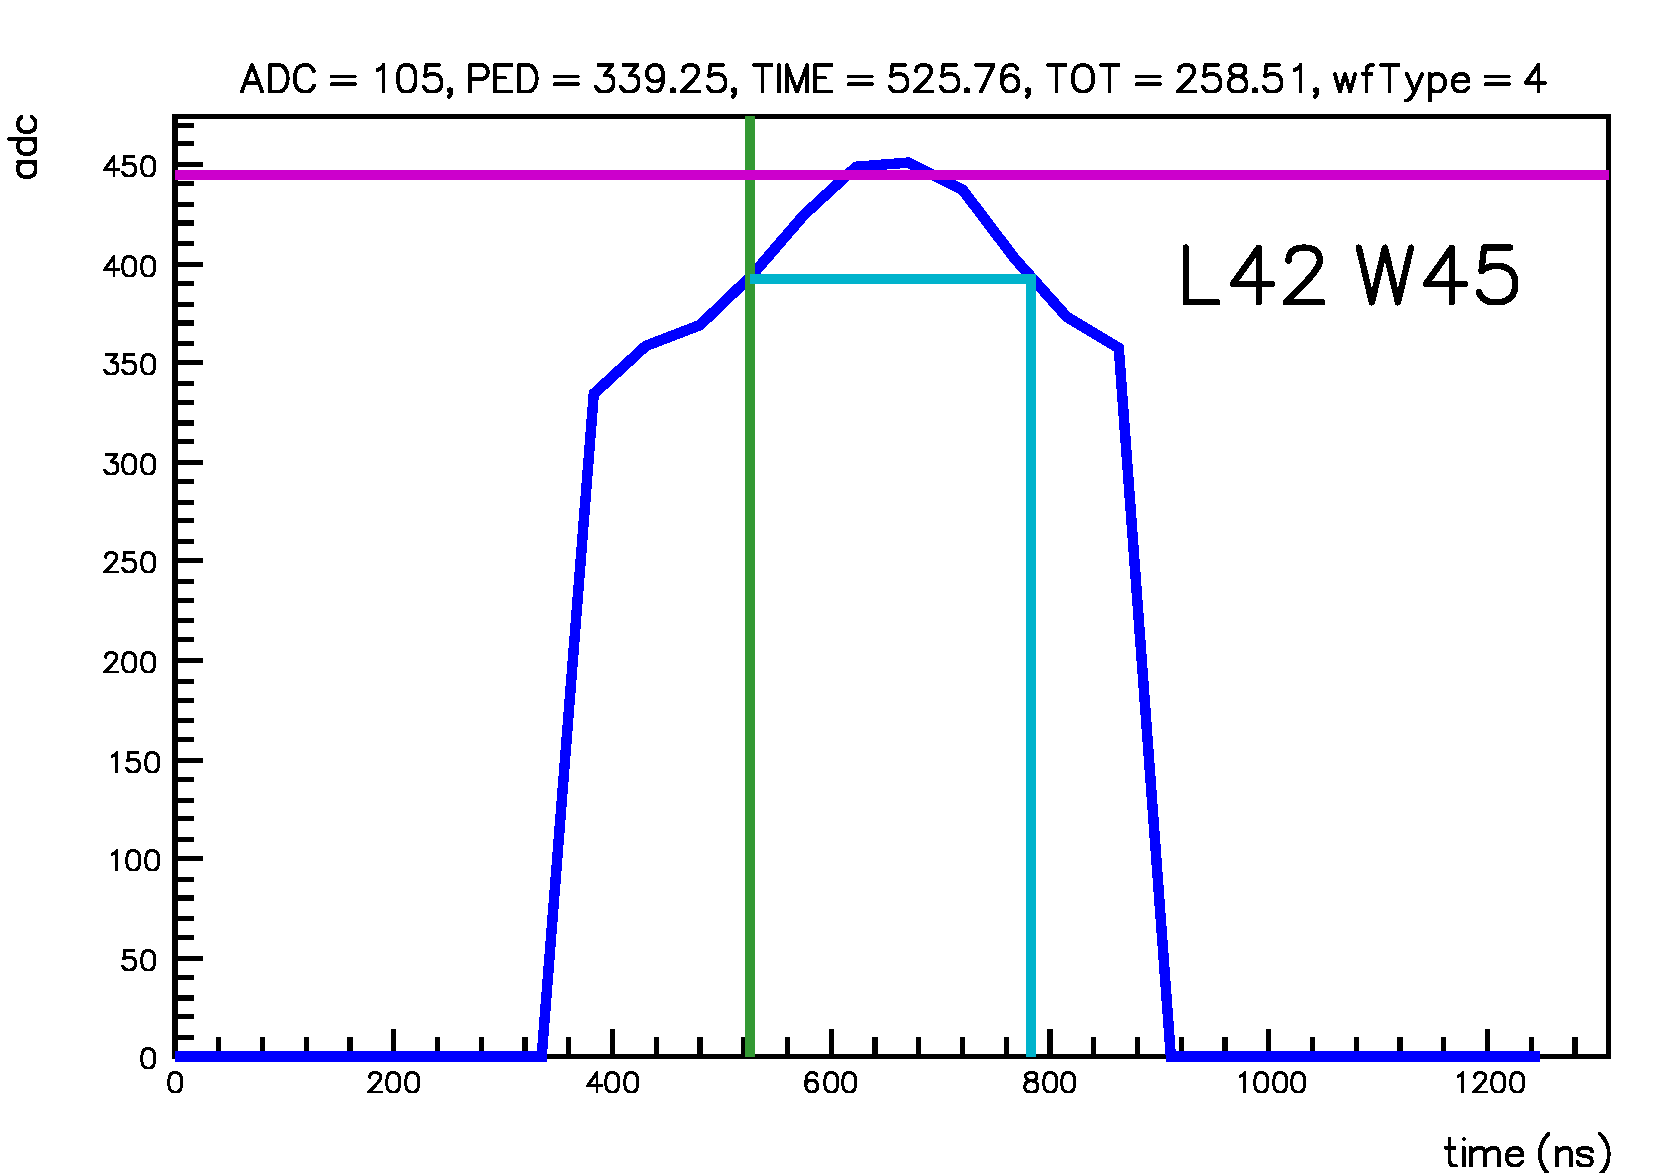
\includegraphics[width=0.45\linewidth]{figures/good_track_but_bad_tot_wf1.pdf} &
                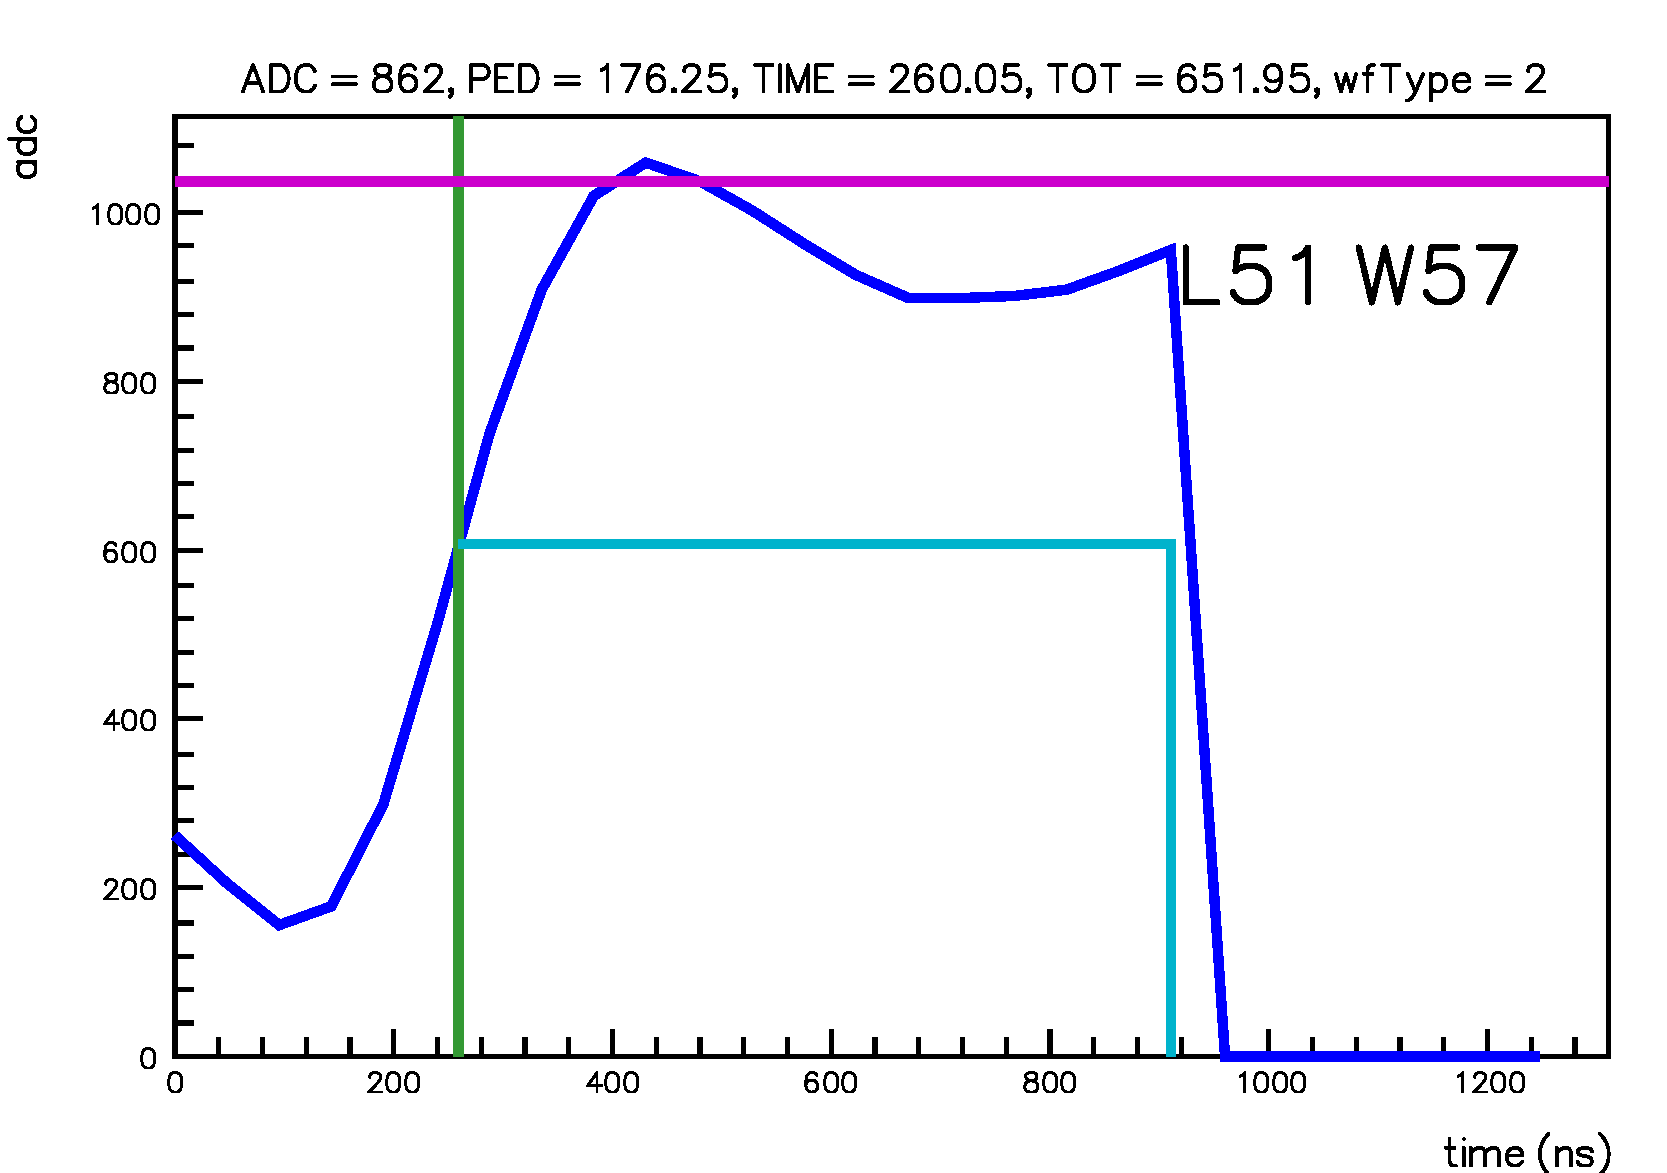
\includegraphics[width=0.45\linewidth]{figures/good_track_but_bad_tot_wf2.pdf}
        \end{tabular}
    \end{minipage}\hfill
    \begin{minipage}{0.4\textwidth}
        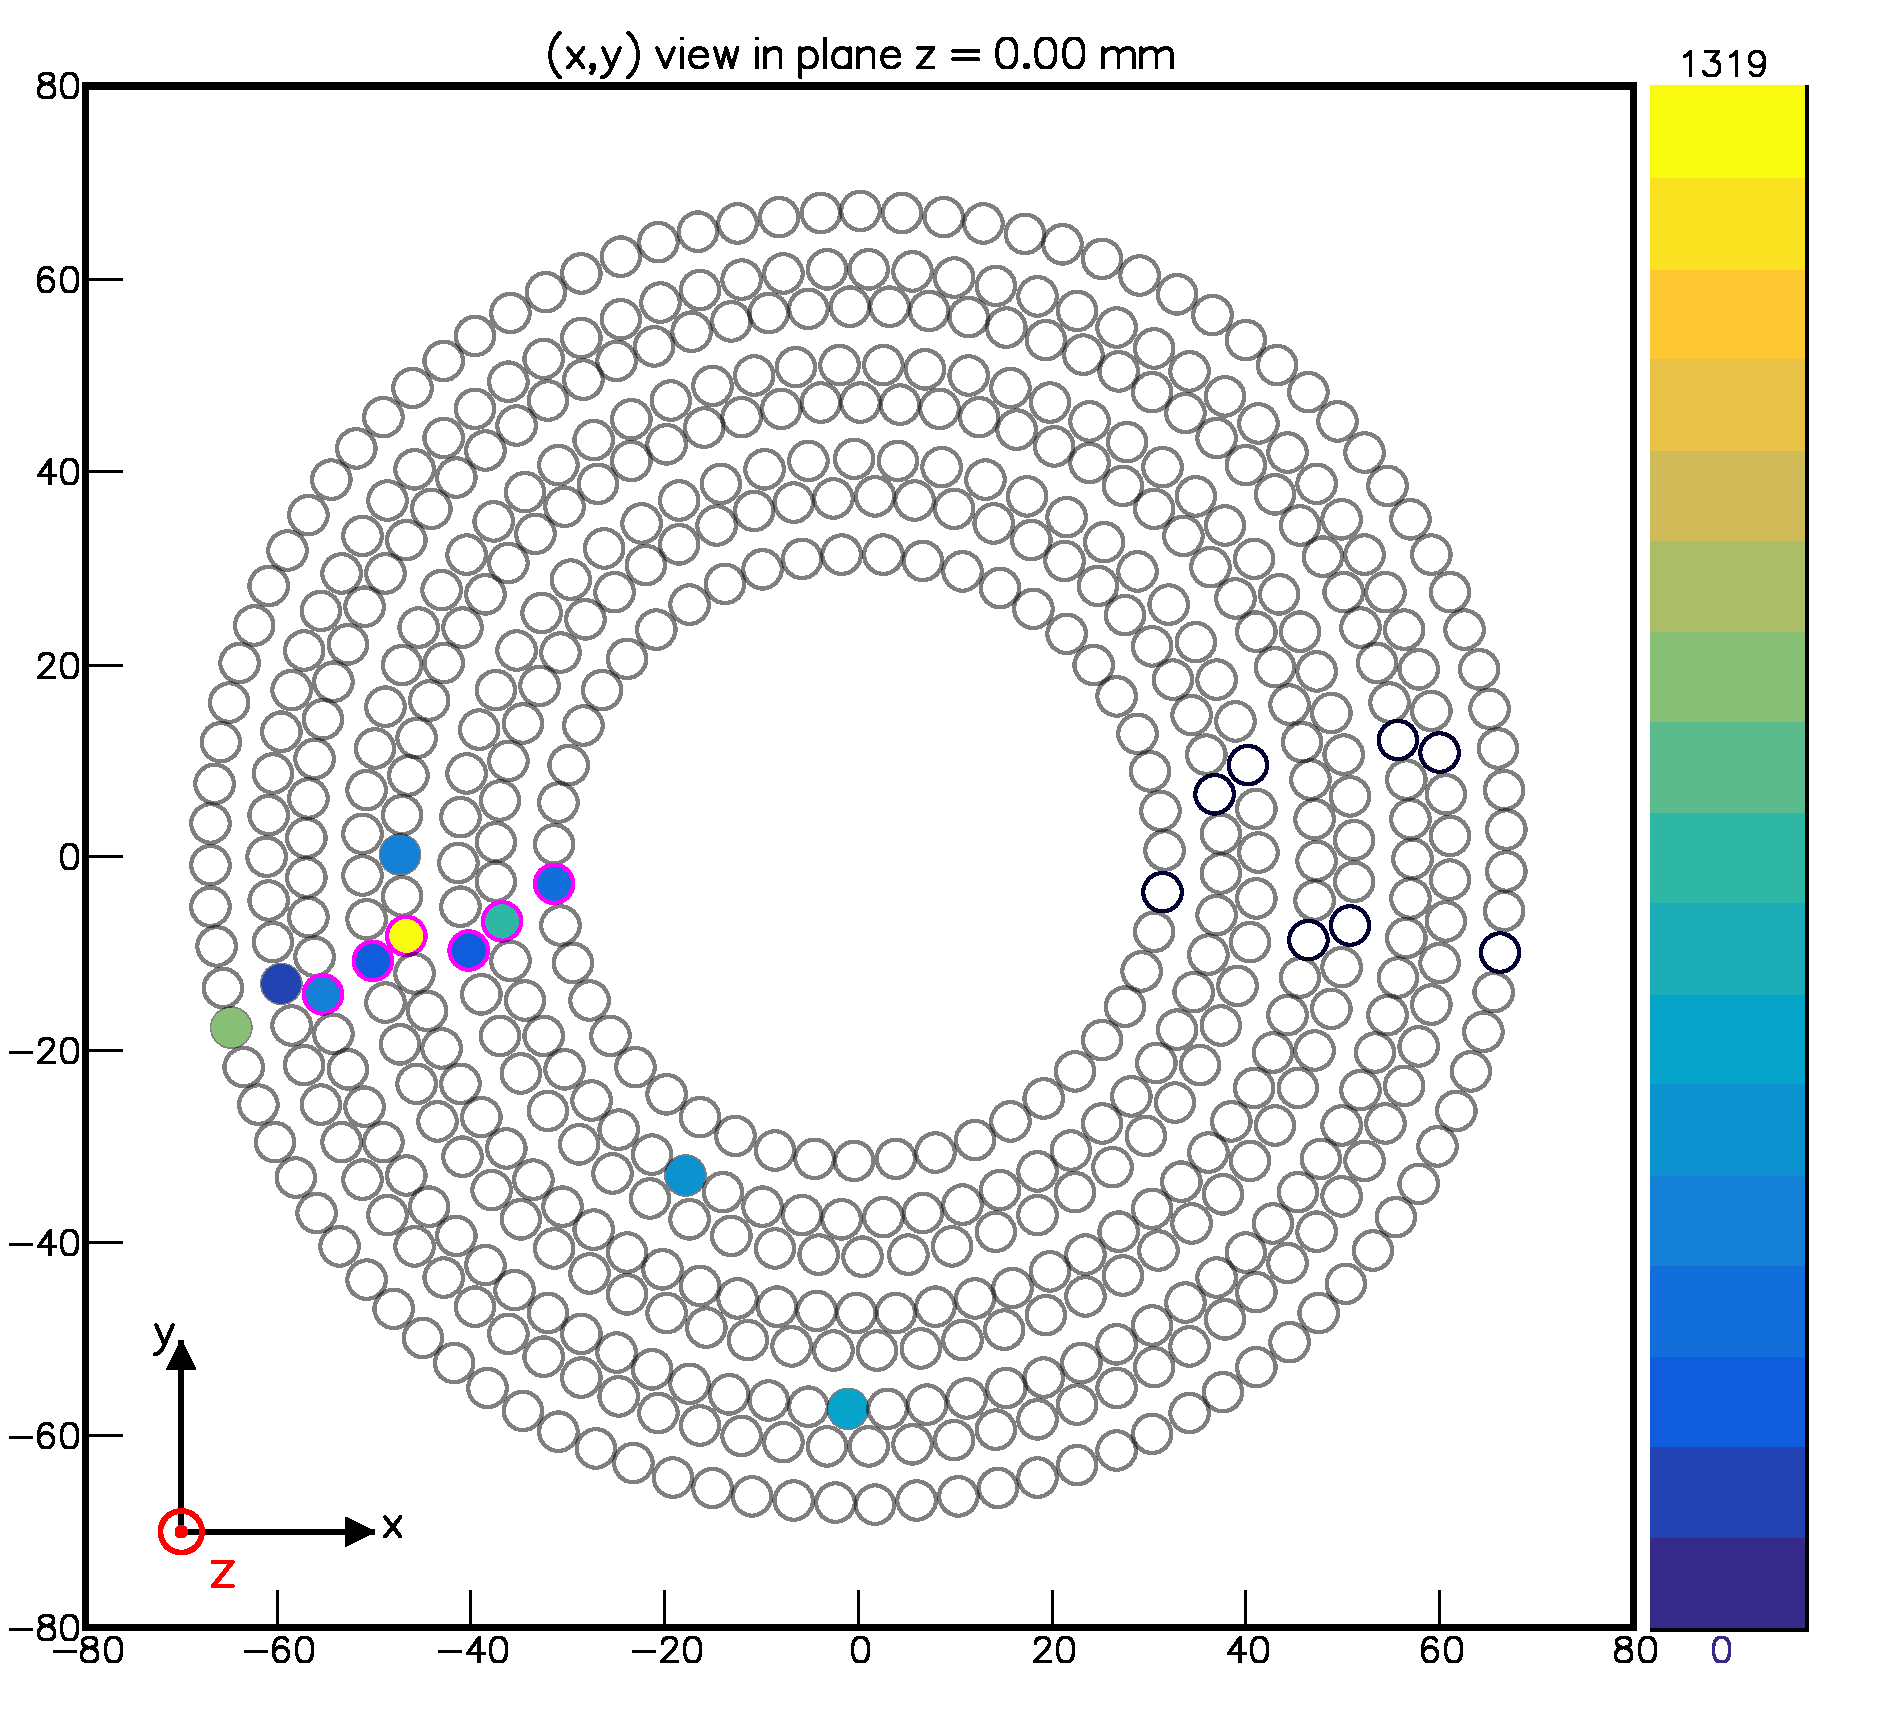
\includegraphics[width=\linewidth]{figures/good_track_but_bad_tot.pdf}
    \end{minipage}

\end{frame}

\begin{frame}{Issue with tracks losing hits 1/2}
    \begin{itemize}
        \item Here, I looked at tracks with at least 6 hits, and I was surprised that we can have missing hits on a whole superlayer
            \begin{itemize}
                \item The waveforms of these missing hits have no issue, there are all type 0
                \item That happens at lot, they are mostly suppressed hits in the Kalman Filter
                \item That suggests that we still need to have a better time and T2D calibration
            \end{itemize}
    \end{itemize}

    \centering

    \begin{tabular}{cc}
        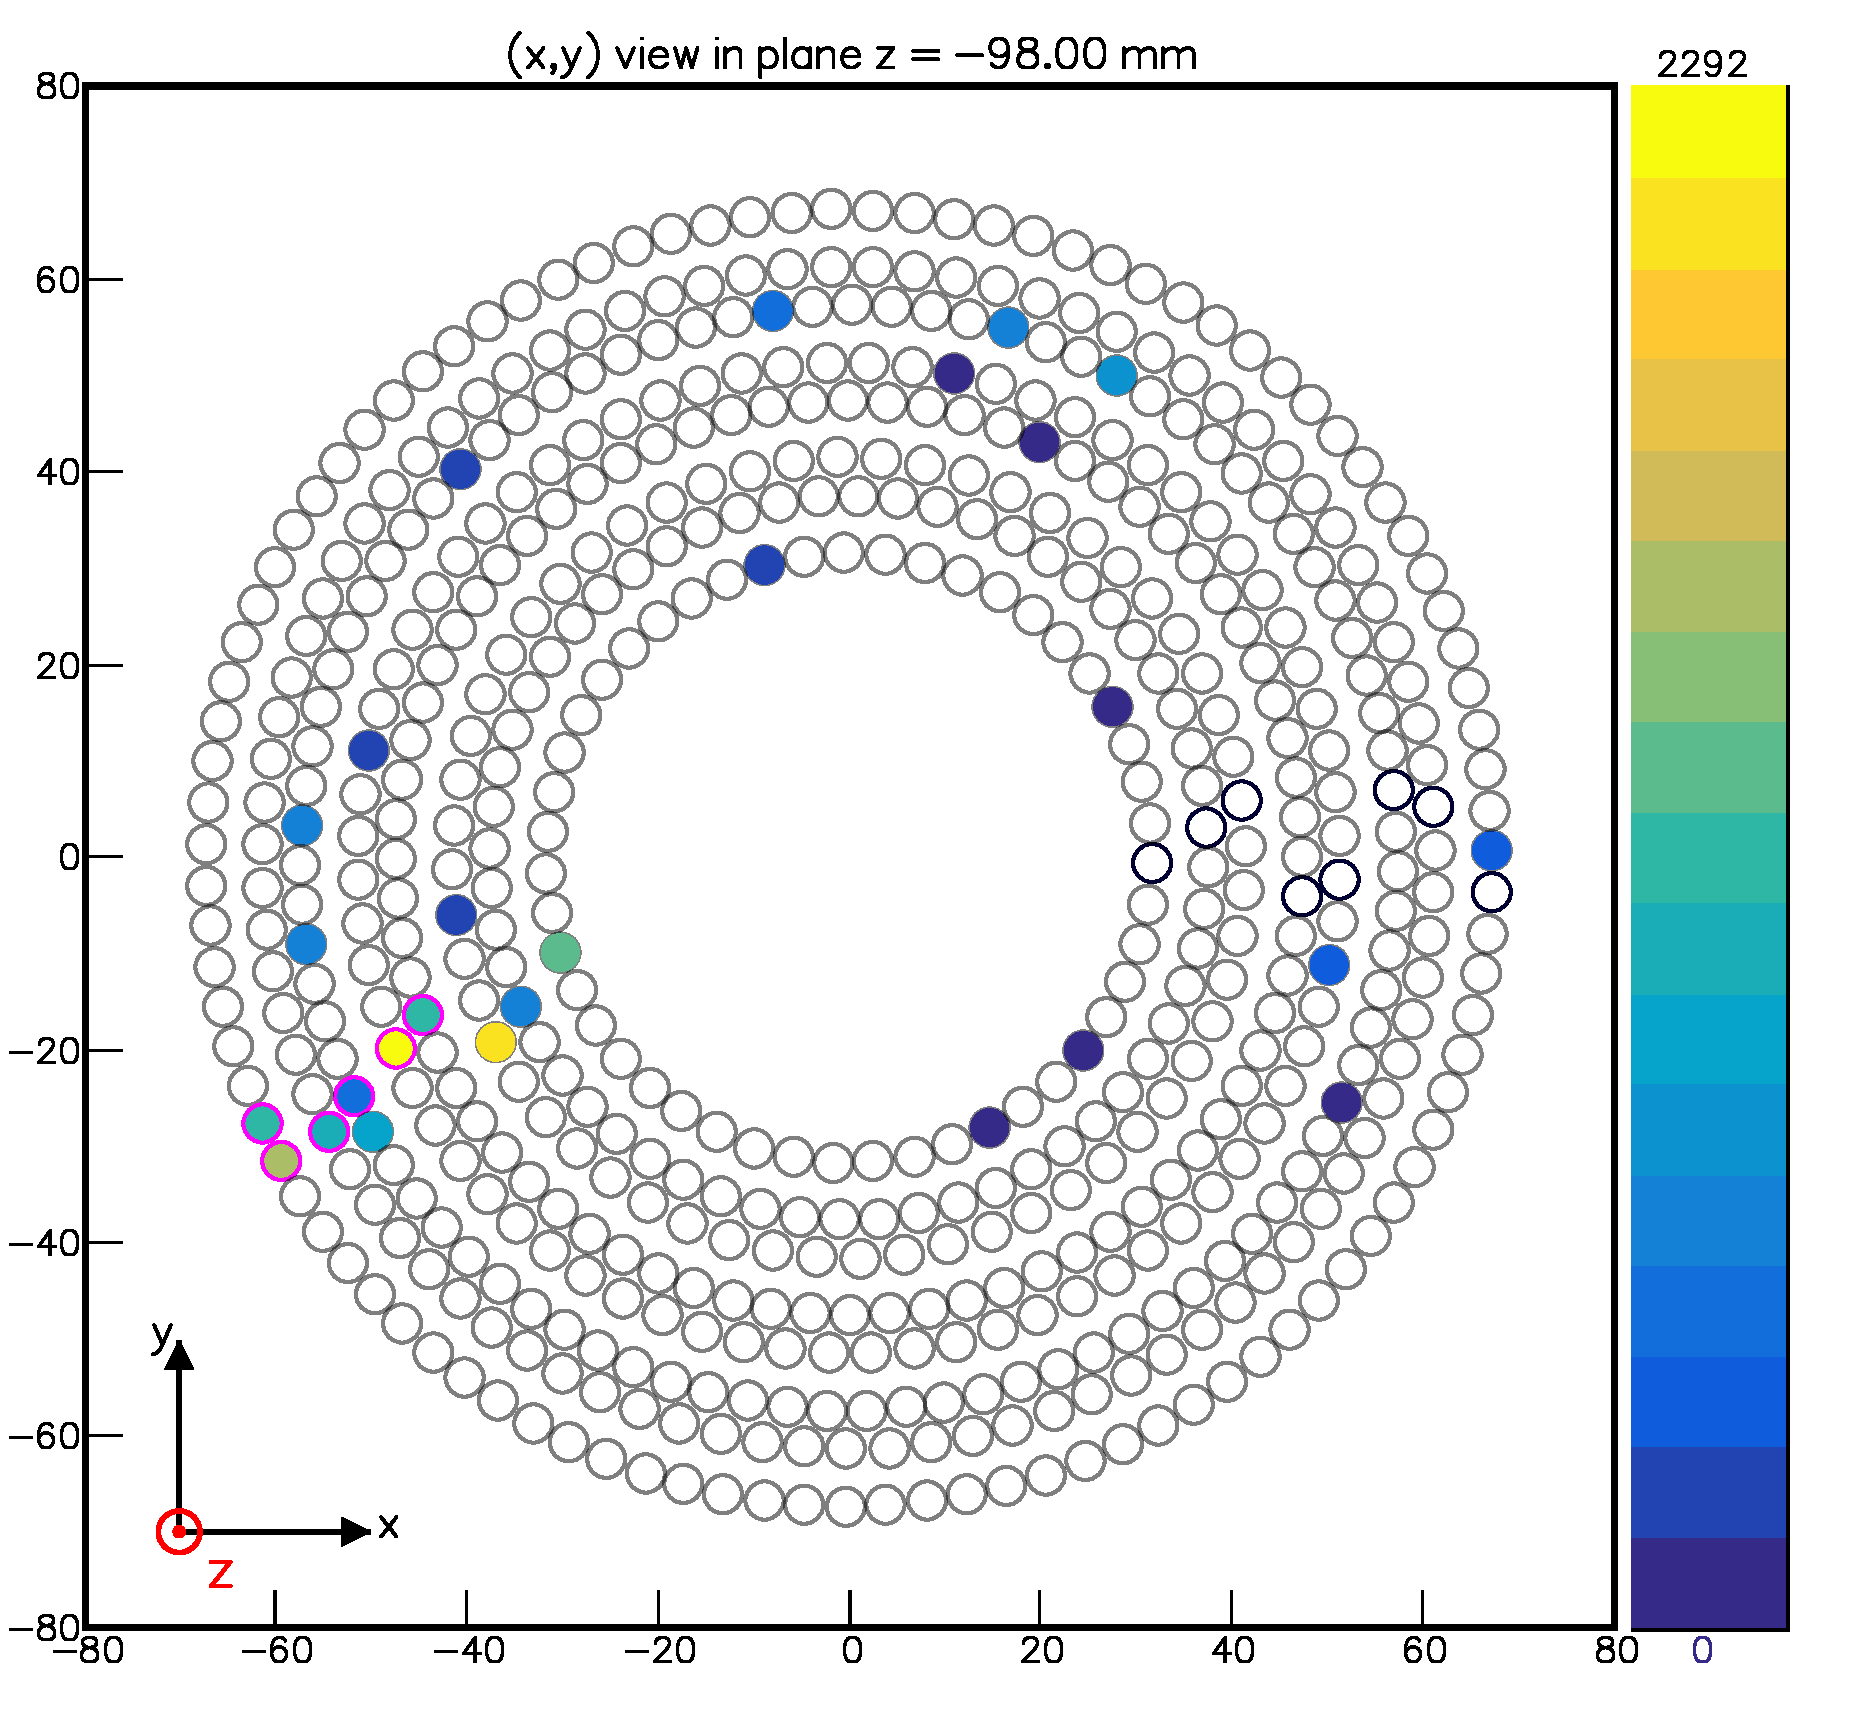
\includegraphics[width=0.35\linewidth]{figures/bad_track_r22712_2gev_missing_hits_num_1.pdf} & 
            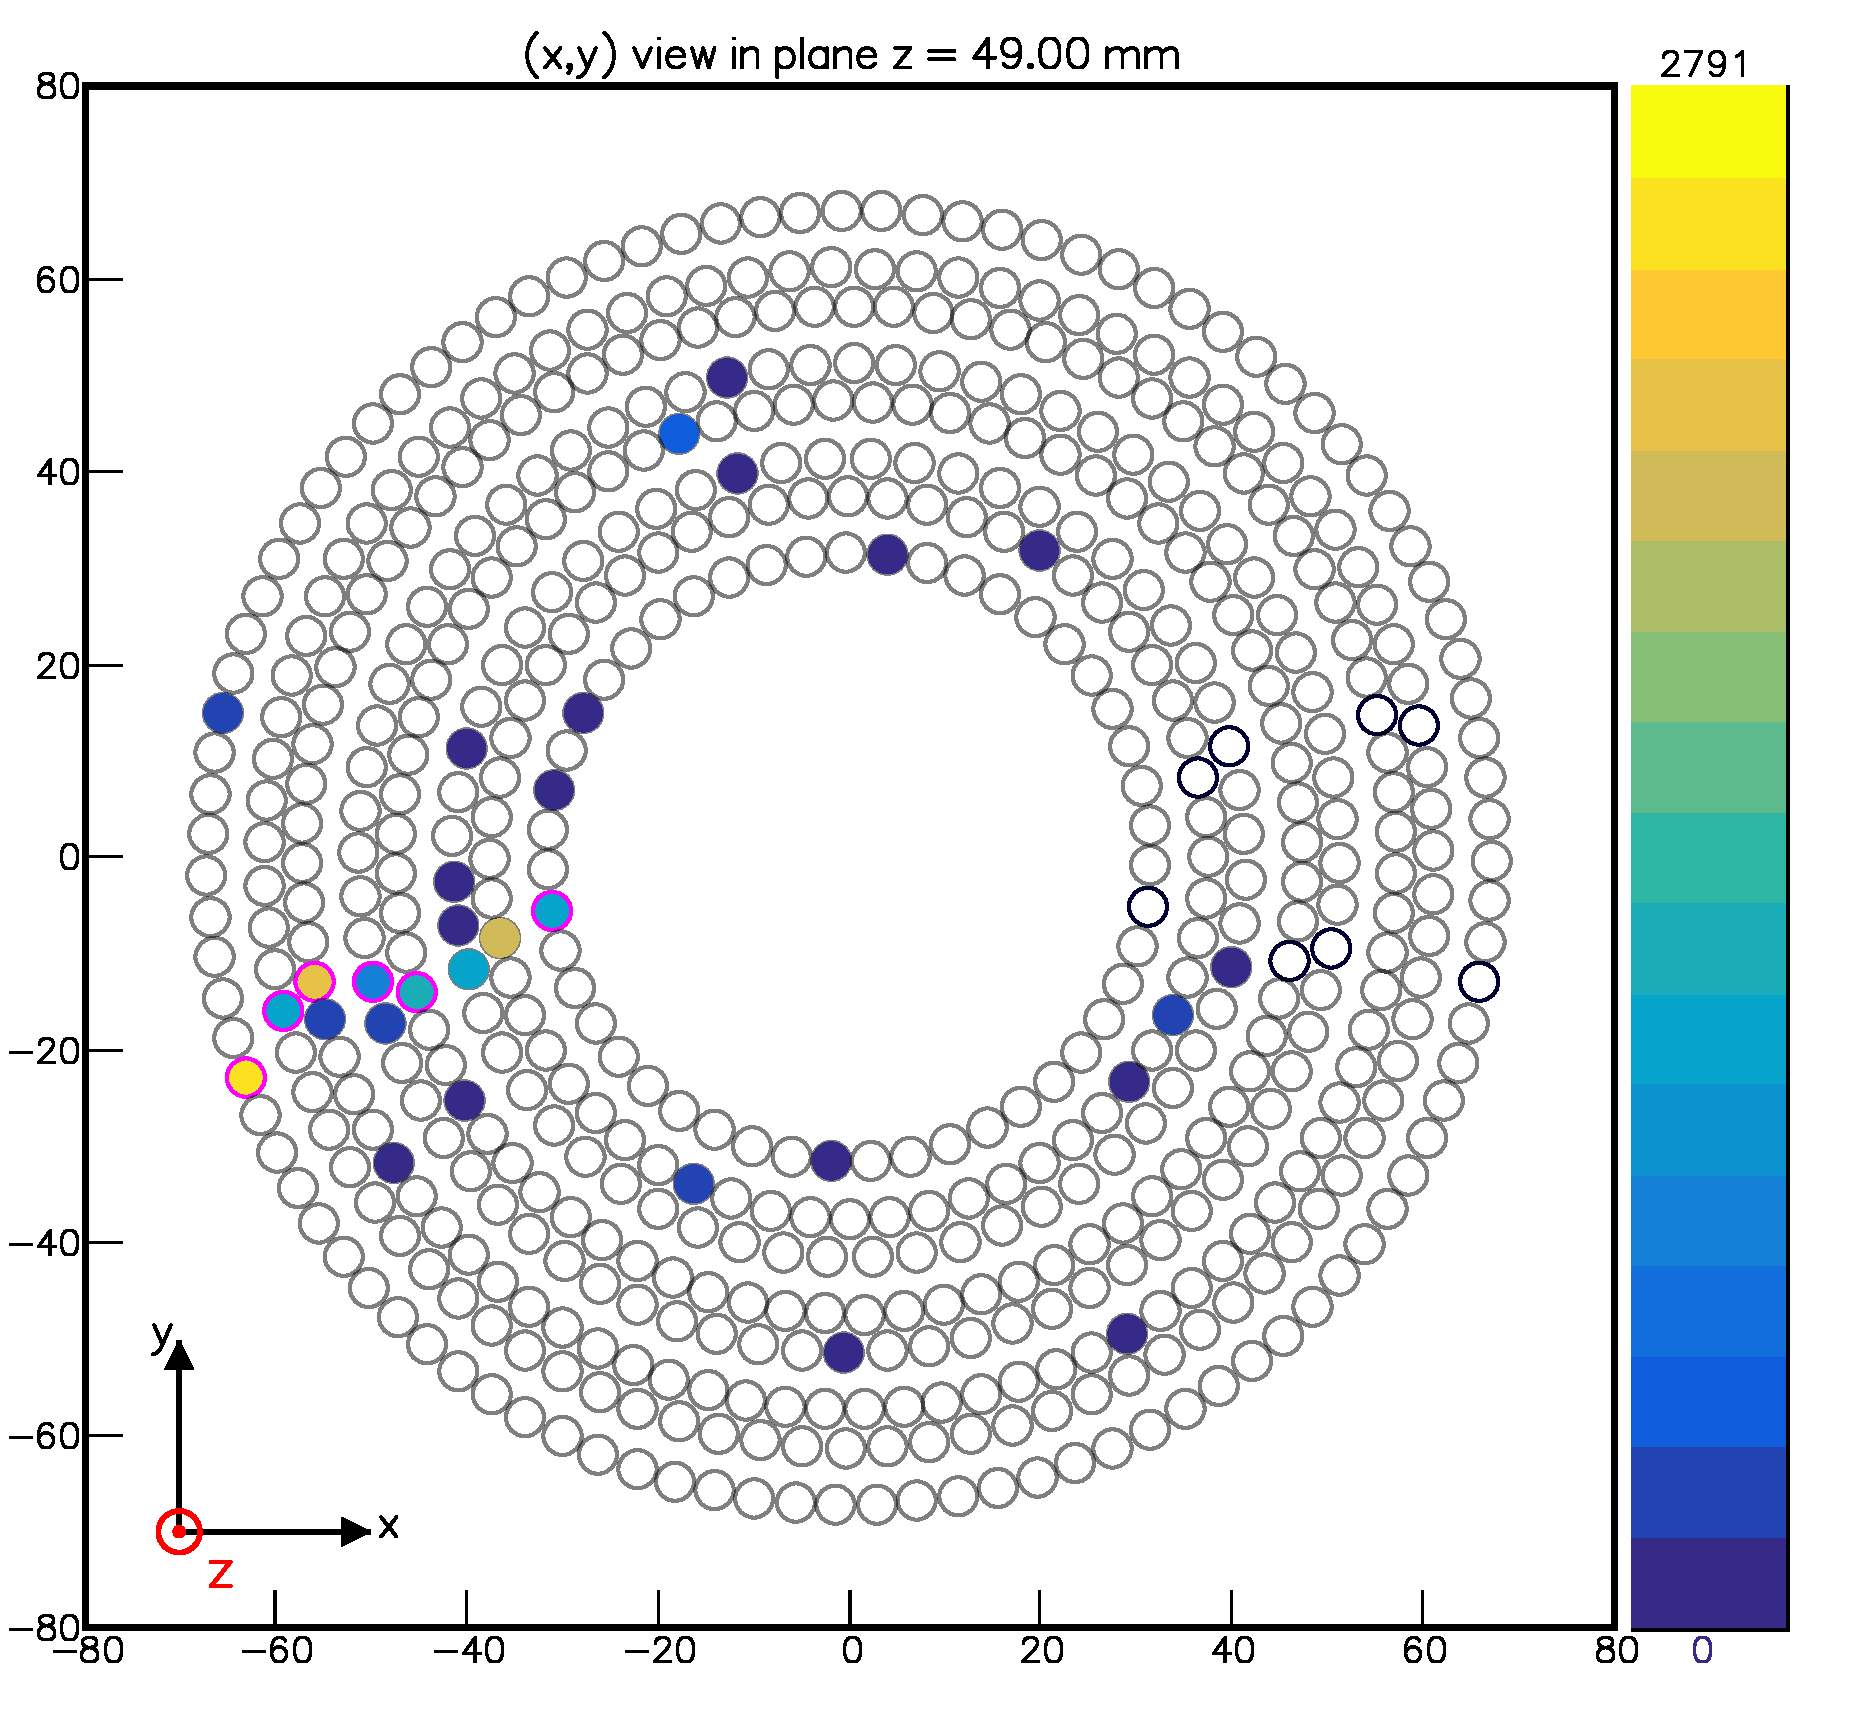
\includegraphics[width=0.35\linewidth]{figures/bad_track_r22712_2gev_missing_hits_num_2.pdf} 
    \end{tabular}

    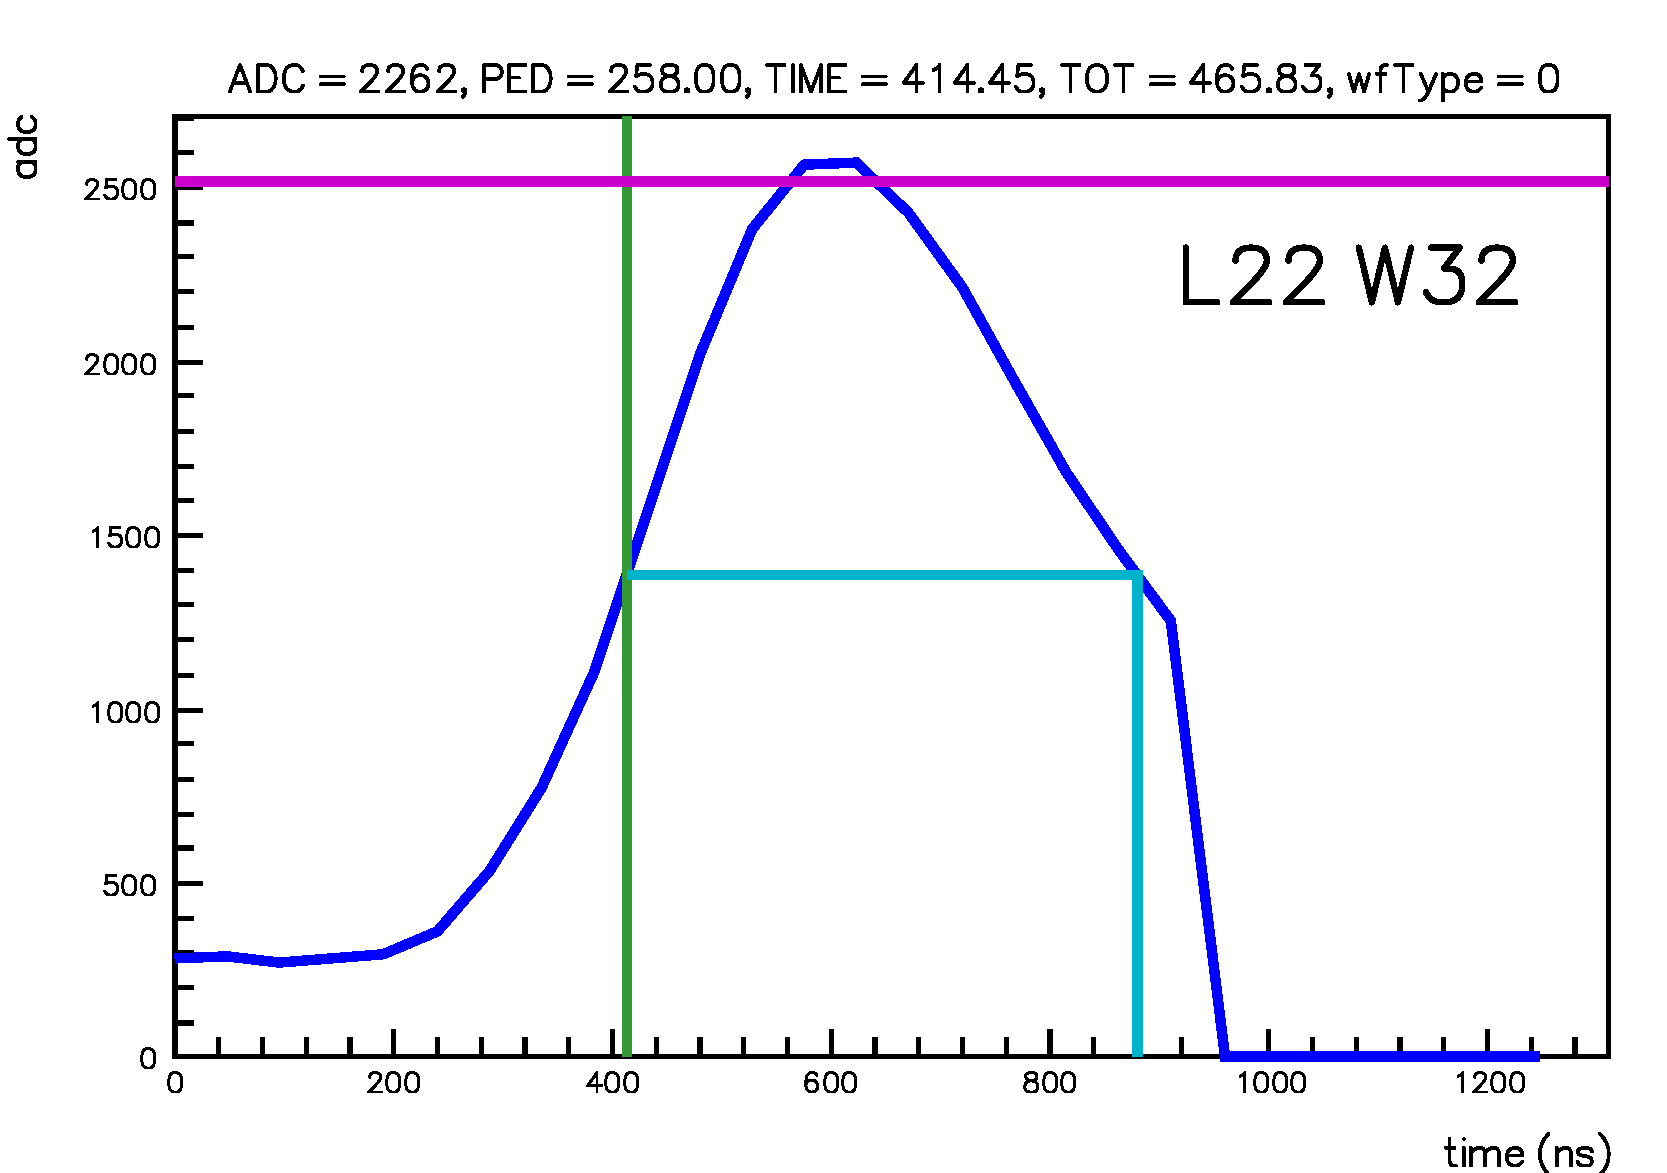
\includegraphics[width=0.22\linewidth]{figures/bad_track_r22712_2gev_missing_hits_num_1_wf_1.pdf}
    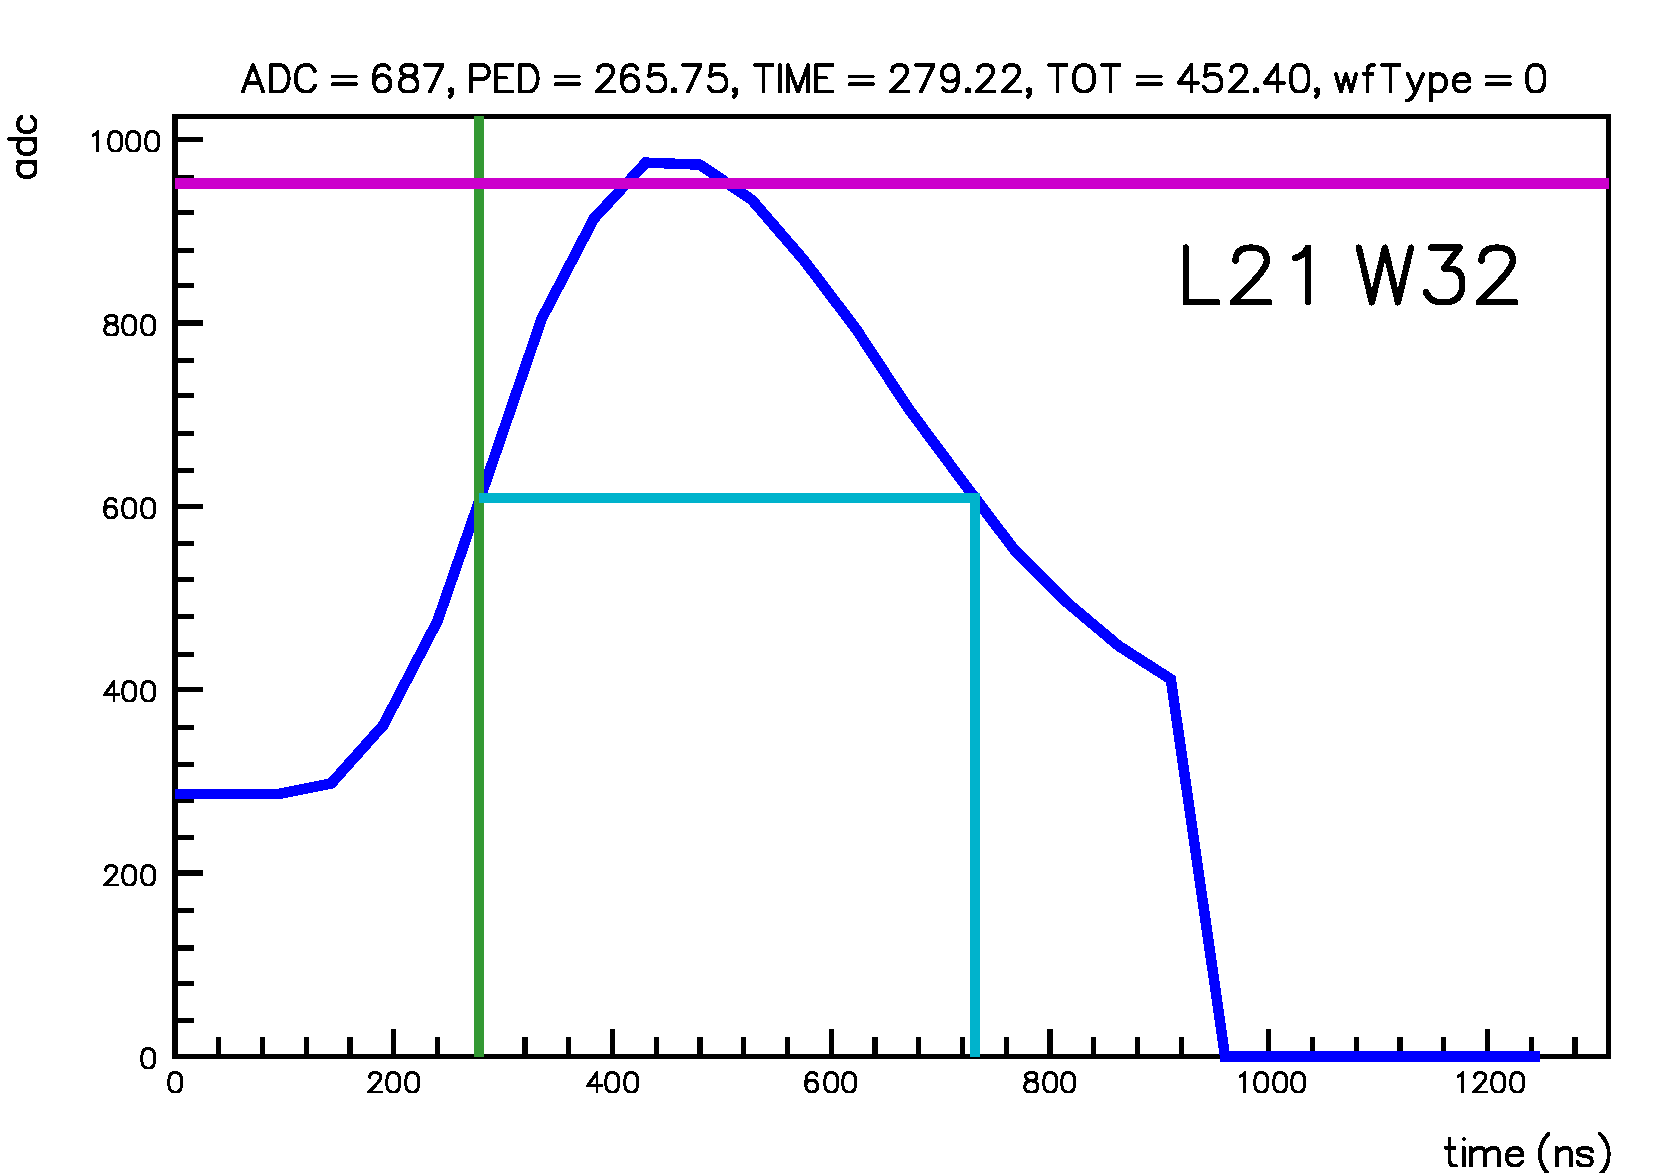
\includegraphics[width=0.22\linewidth]{figures/bad_track_r22712_2gev_missing_hits_num_1_wf_2.pdf}
    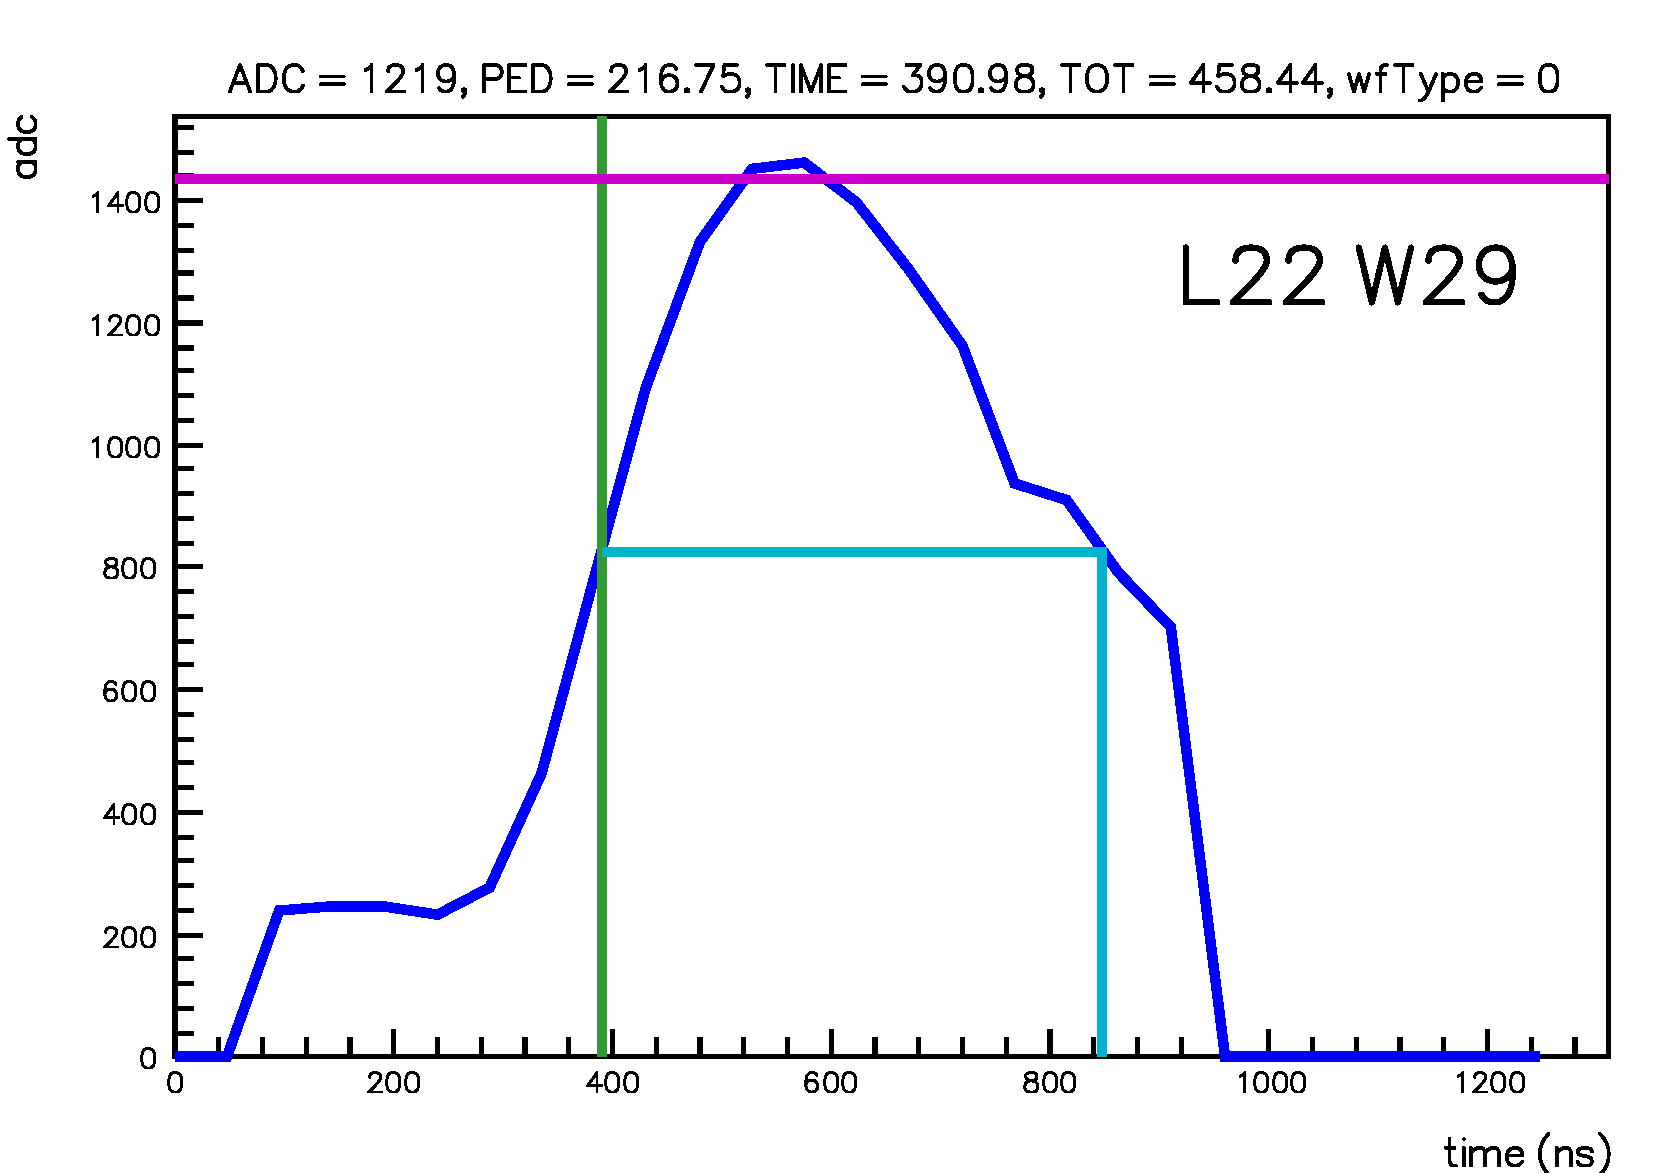
\includegraphics[width=0.22\linewidth]{figures/bad_track_r22712_2gev_missing_hits_num_2_wf_1.pdf}
    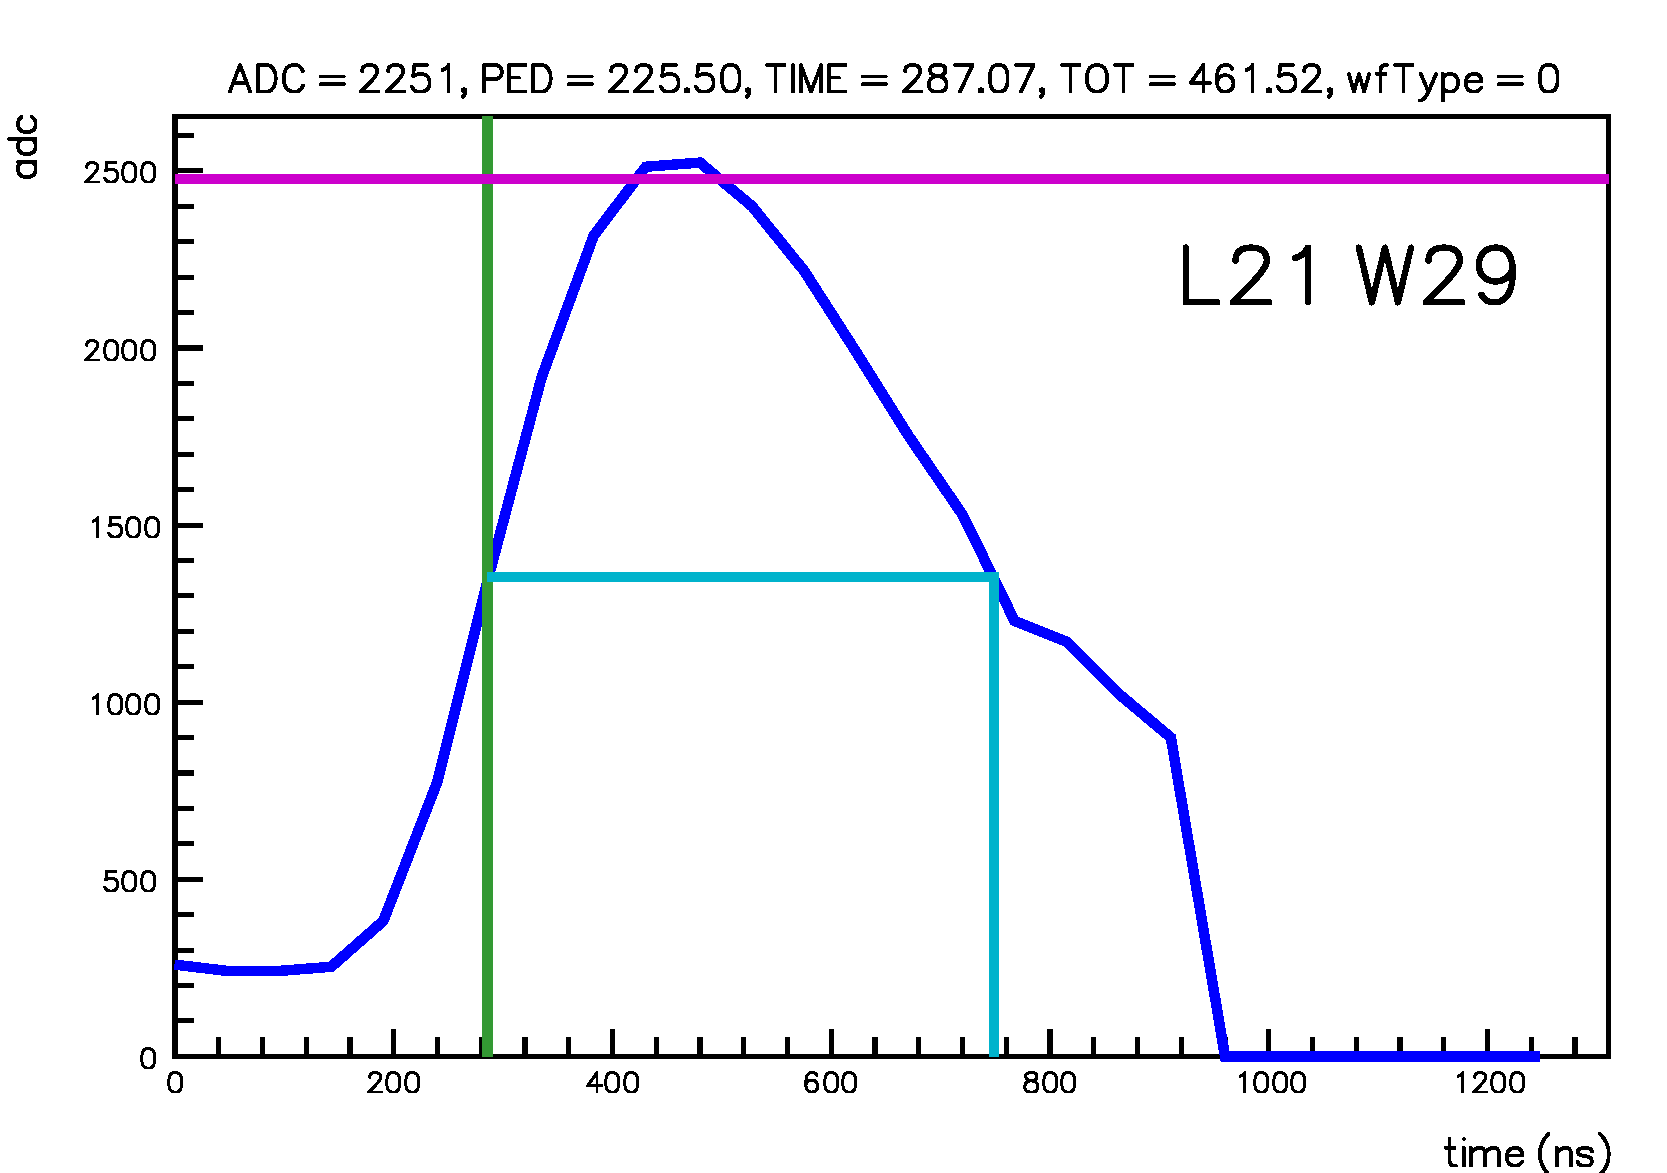
\includegraphics[width=0.22\linewidth]{figures/bad_track_r22712_2gev_missing_hits_num_2_wf_2.pdf}

\end{frame}

\begin{frame}{Issue with tracks losing hits 2/2}
    \begin{itemize}
        \item Worst case scenario: not even a hit on the first 4 layers.
        \item In my next analysis, I will only consider tracks with at least 6 or 7 layers reached (before, I was just assuming that having more hits, meant reaching all layers)
        \item Until now, all these observations were made on run 22712, 2 GeV, 50 nA: things get worst at 10.6 GeV
    \end{itemize}

    \centering
    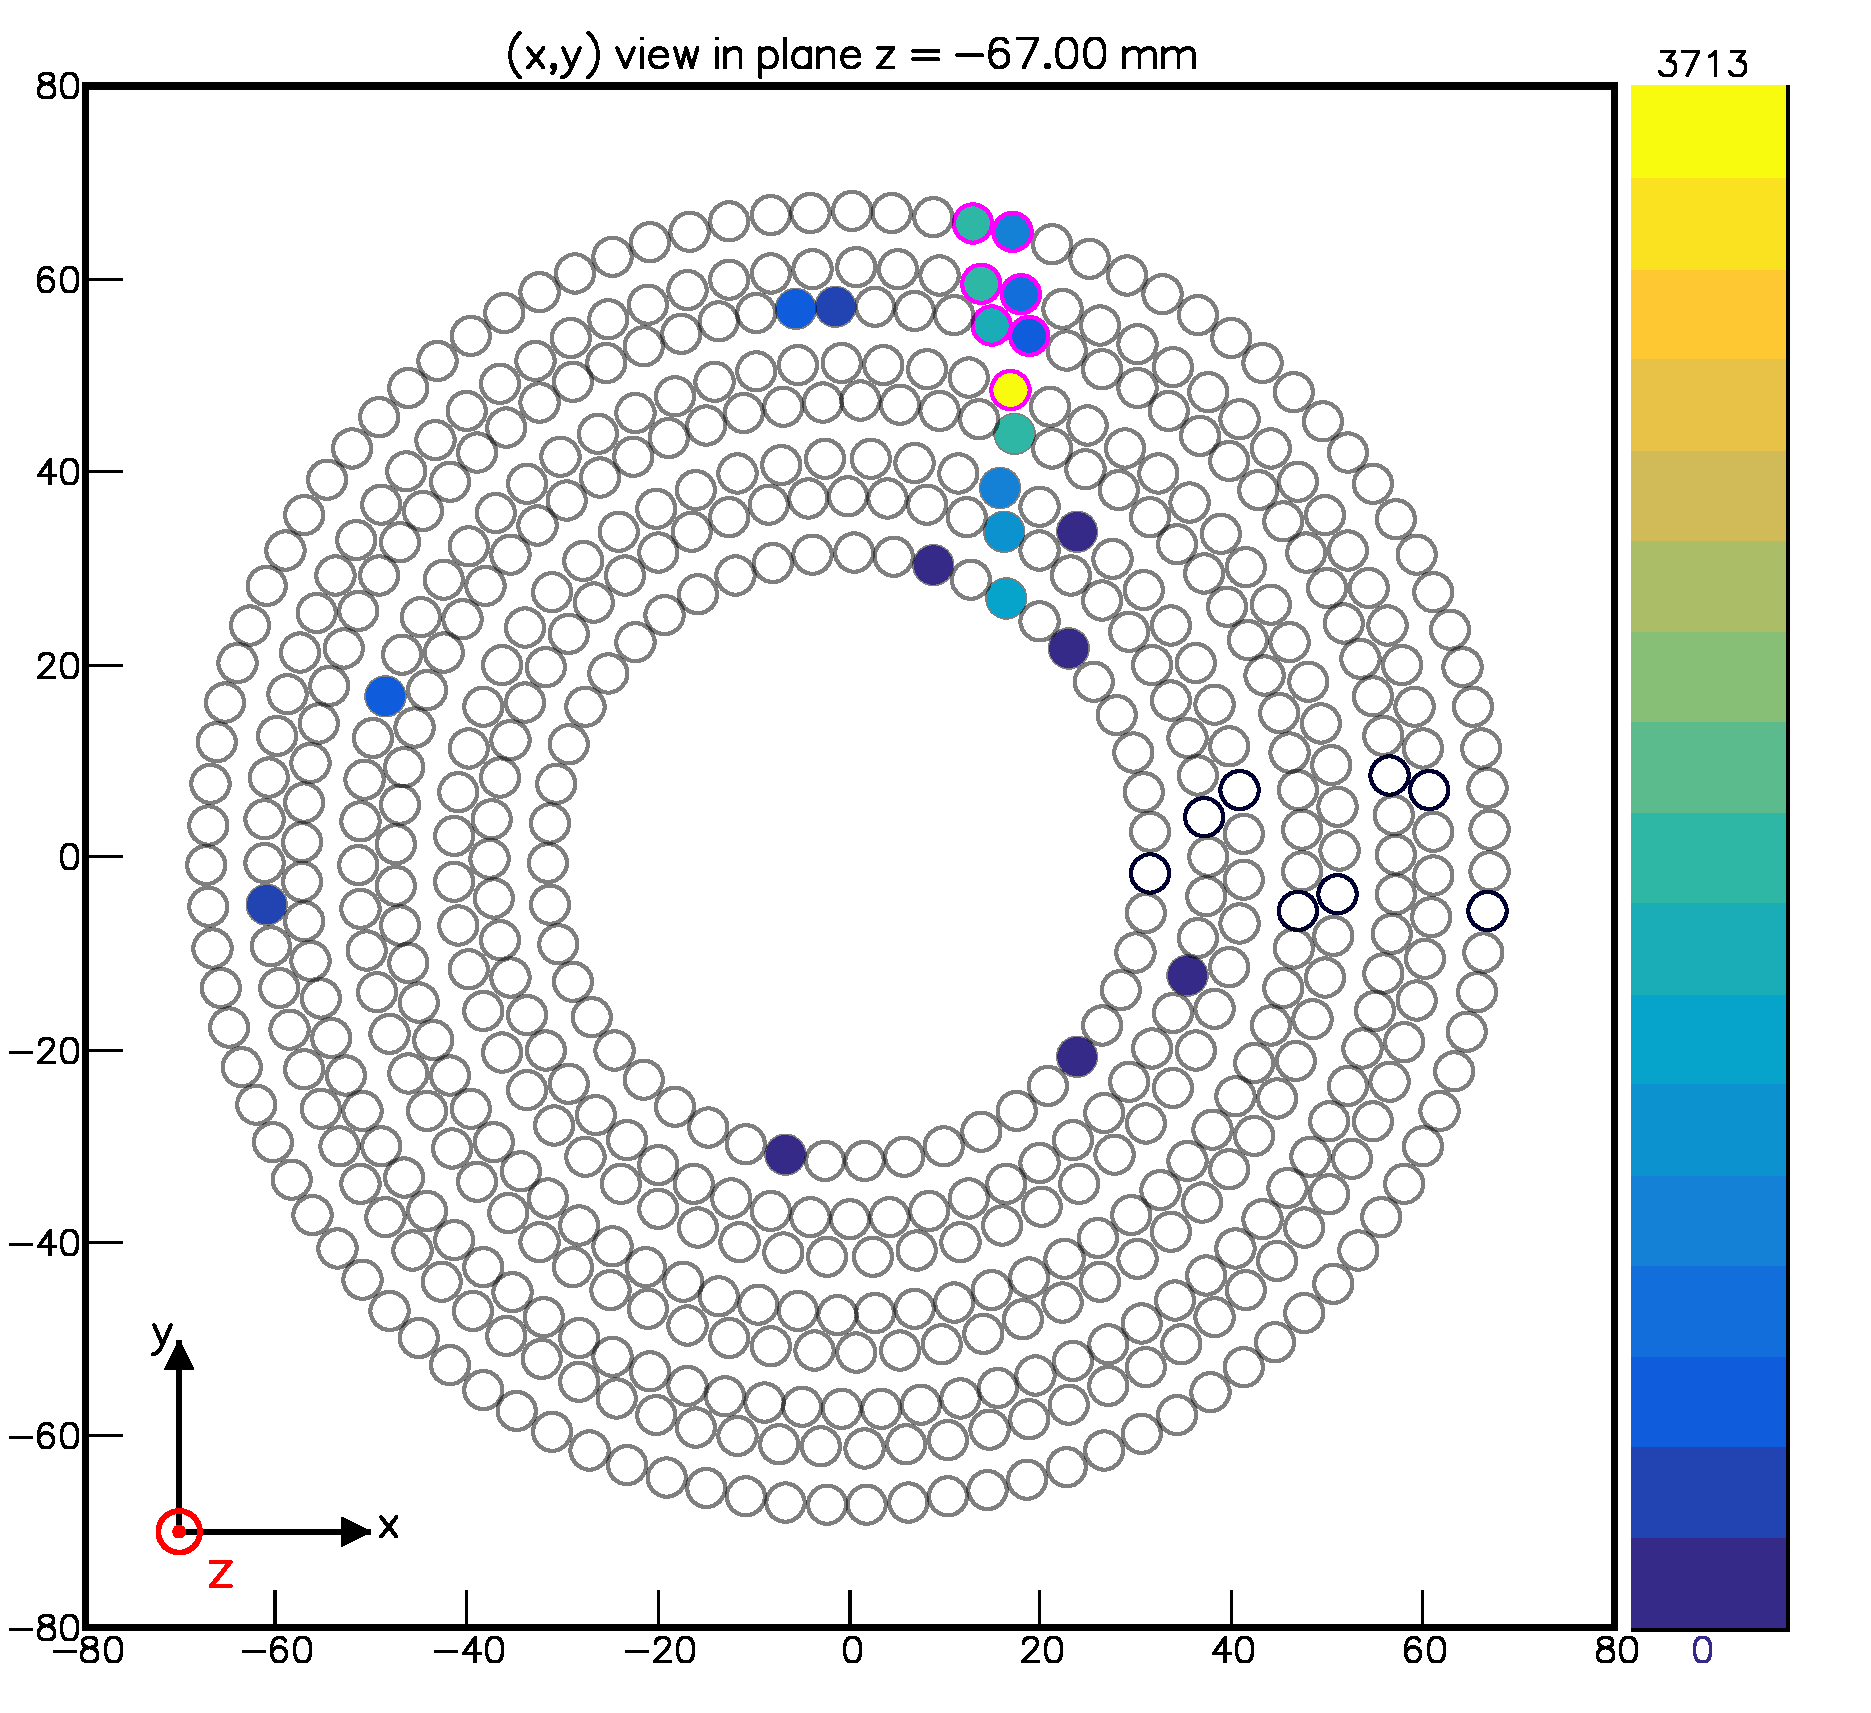
\includegraphics[width=0.5\linewidth]{figures/bad_track_r22712_2gev_missing_hits_num_3_worst_case.pdf}

\end{frame}

\begin{frame}{Track reconstructed in 10.6 GeV data 1/3}

    \begin{itemize}
        \item Example on run 22172, 4He, 10.6 GeV, 325 nA
        \item Here I was expecting to reconstruct the high deposited energy
        \item Instead, I reconstructed an artifact (magenta circles)
            \begin{itemize}
                \item Most of the saturated hits may seem late, I just think they need their own t0 calibration (what is not done yet)
                \item Their ToT do not really make sense, and I should have removed the cut on the ToT for these signals
            \end{itemize}
    \end{itemize}

    \begin{minipage}{0.4\textwidth}
        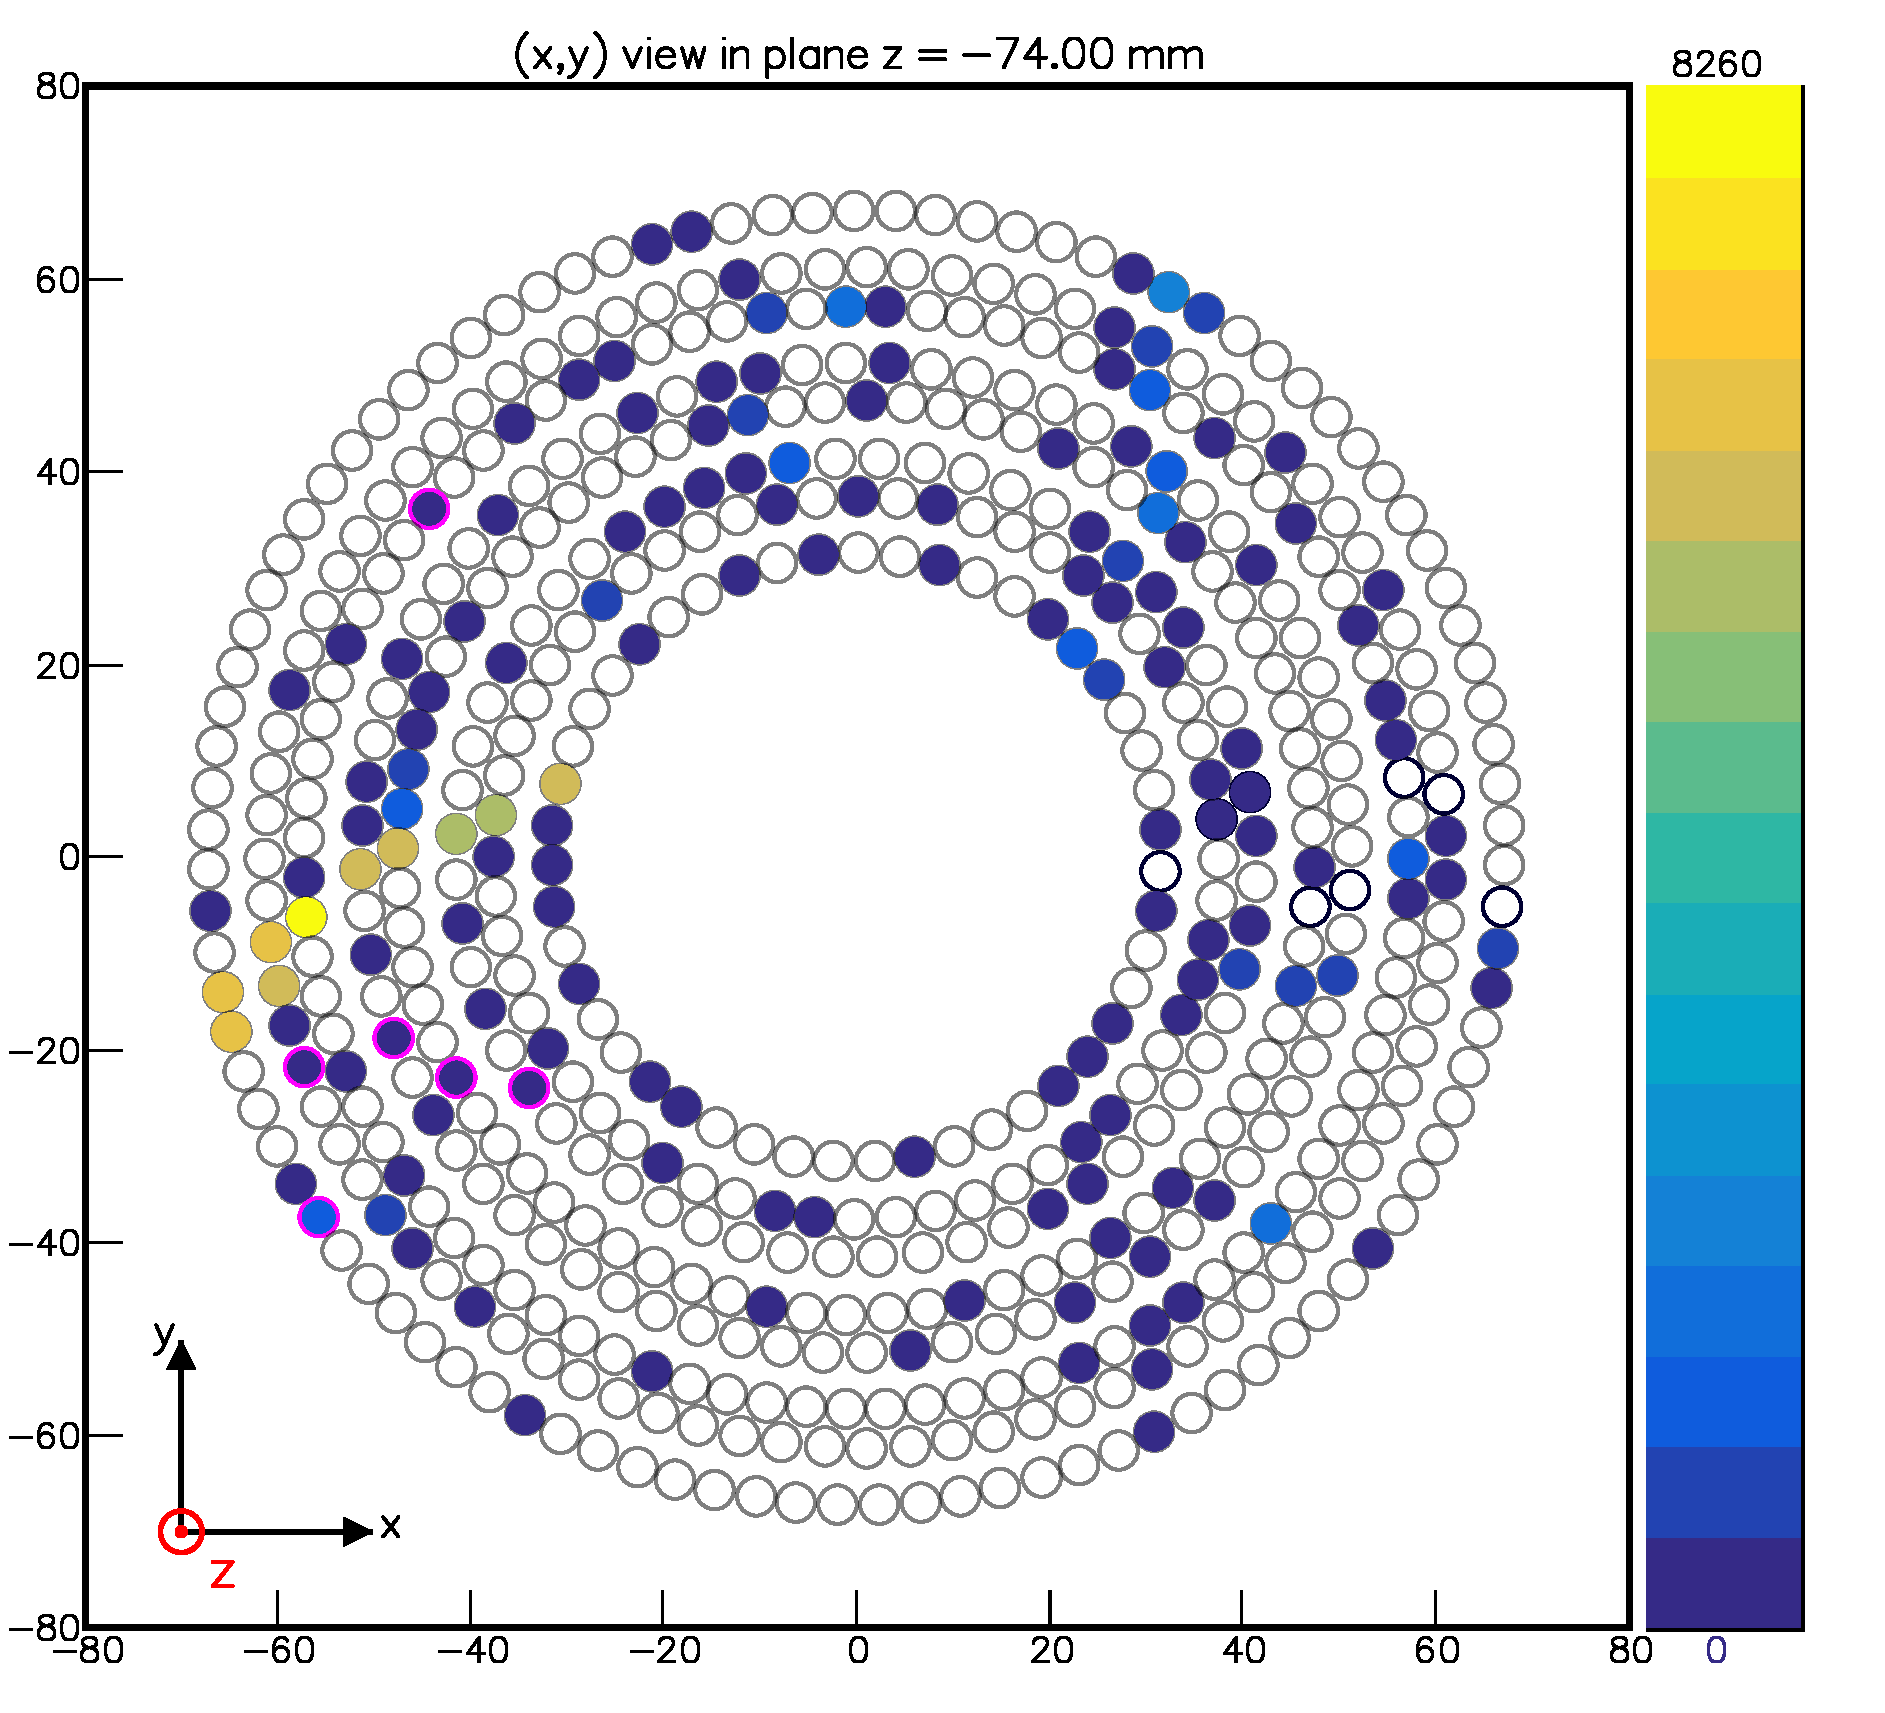
\includegraphics[width=\linewidth]{figures/issue_with_helium_run_num_1.pdf}
    \end{minipage}
    \begin{minipage}{0.58\textwidth}
        \begin{tabular}{cc}
            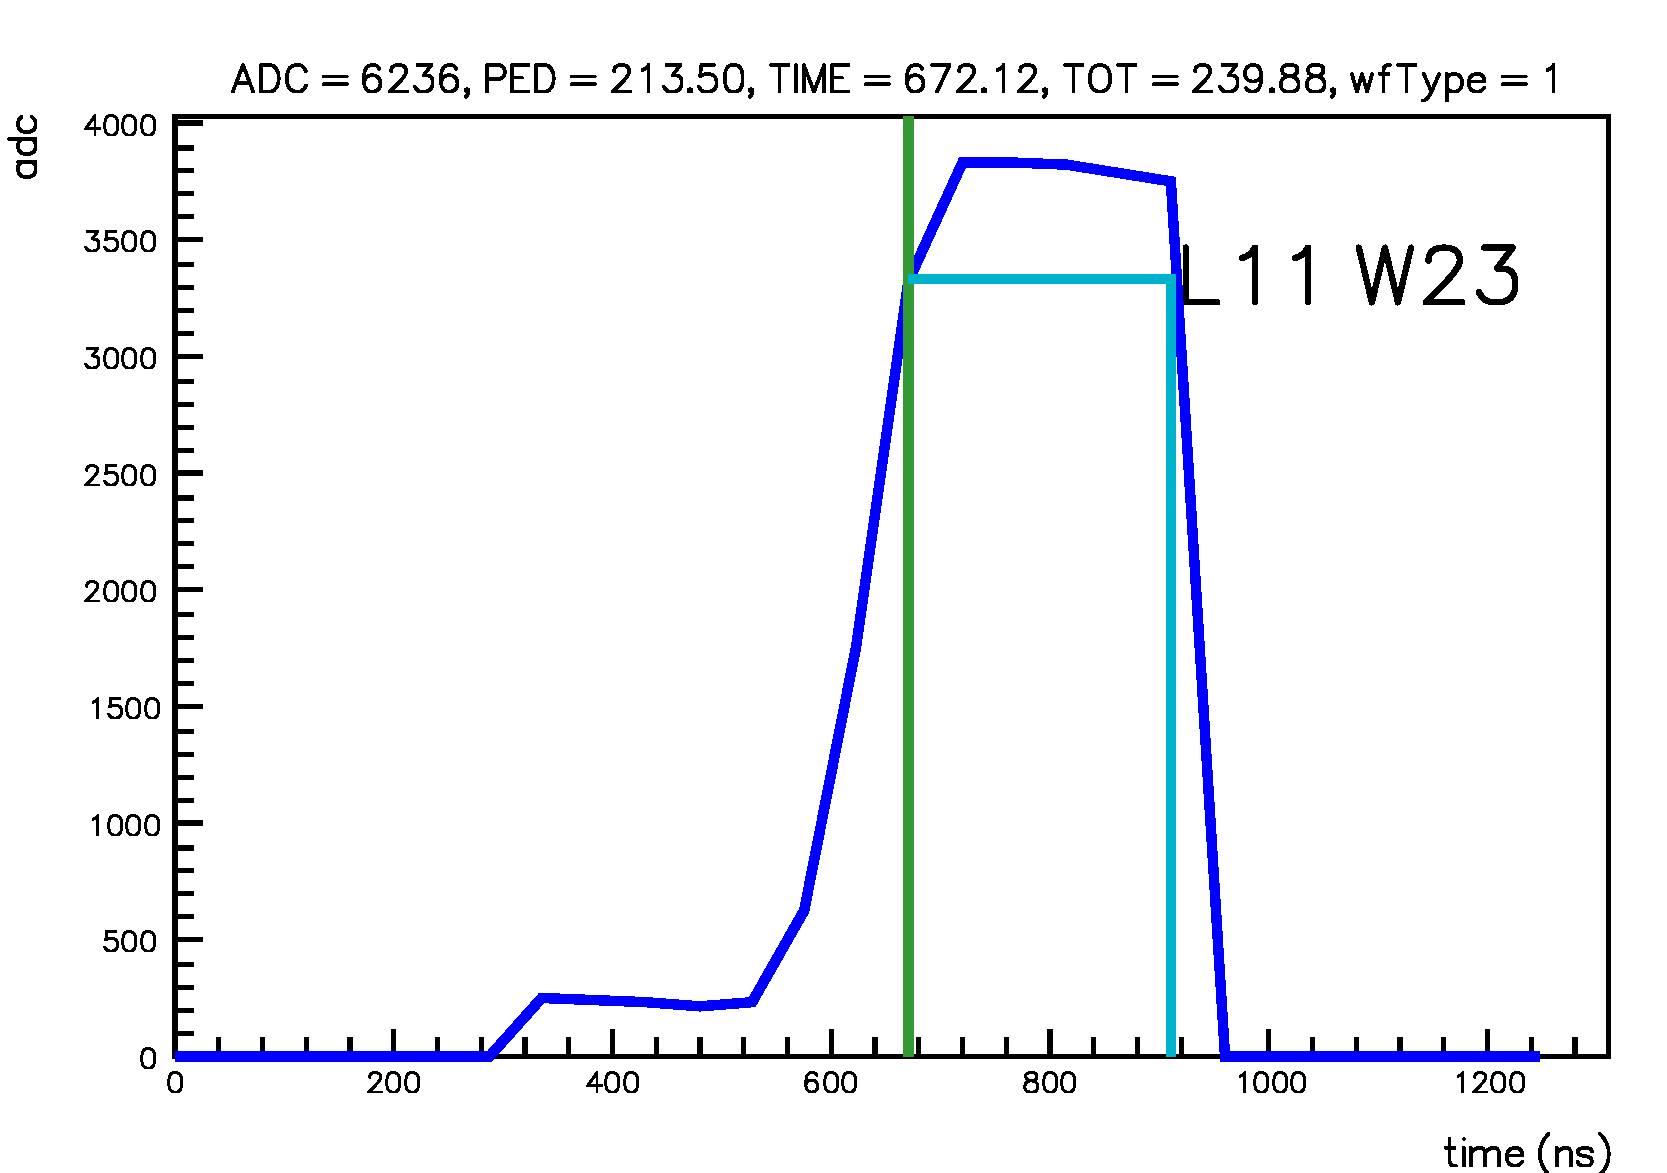
\includegraphics[width=0.45\textwidth]{figures/issue_with_helium_run_num_1_wf1.pdf} &
                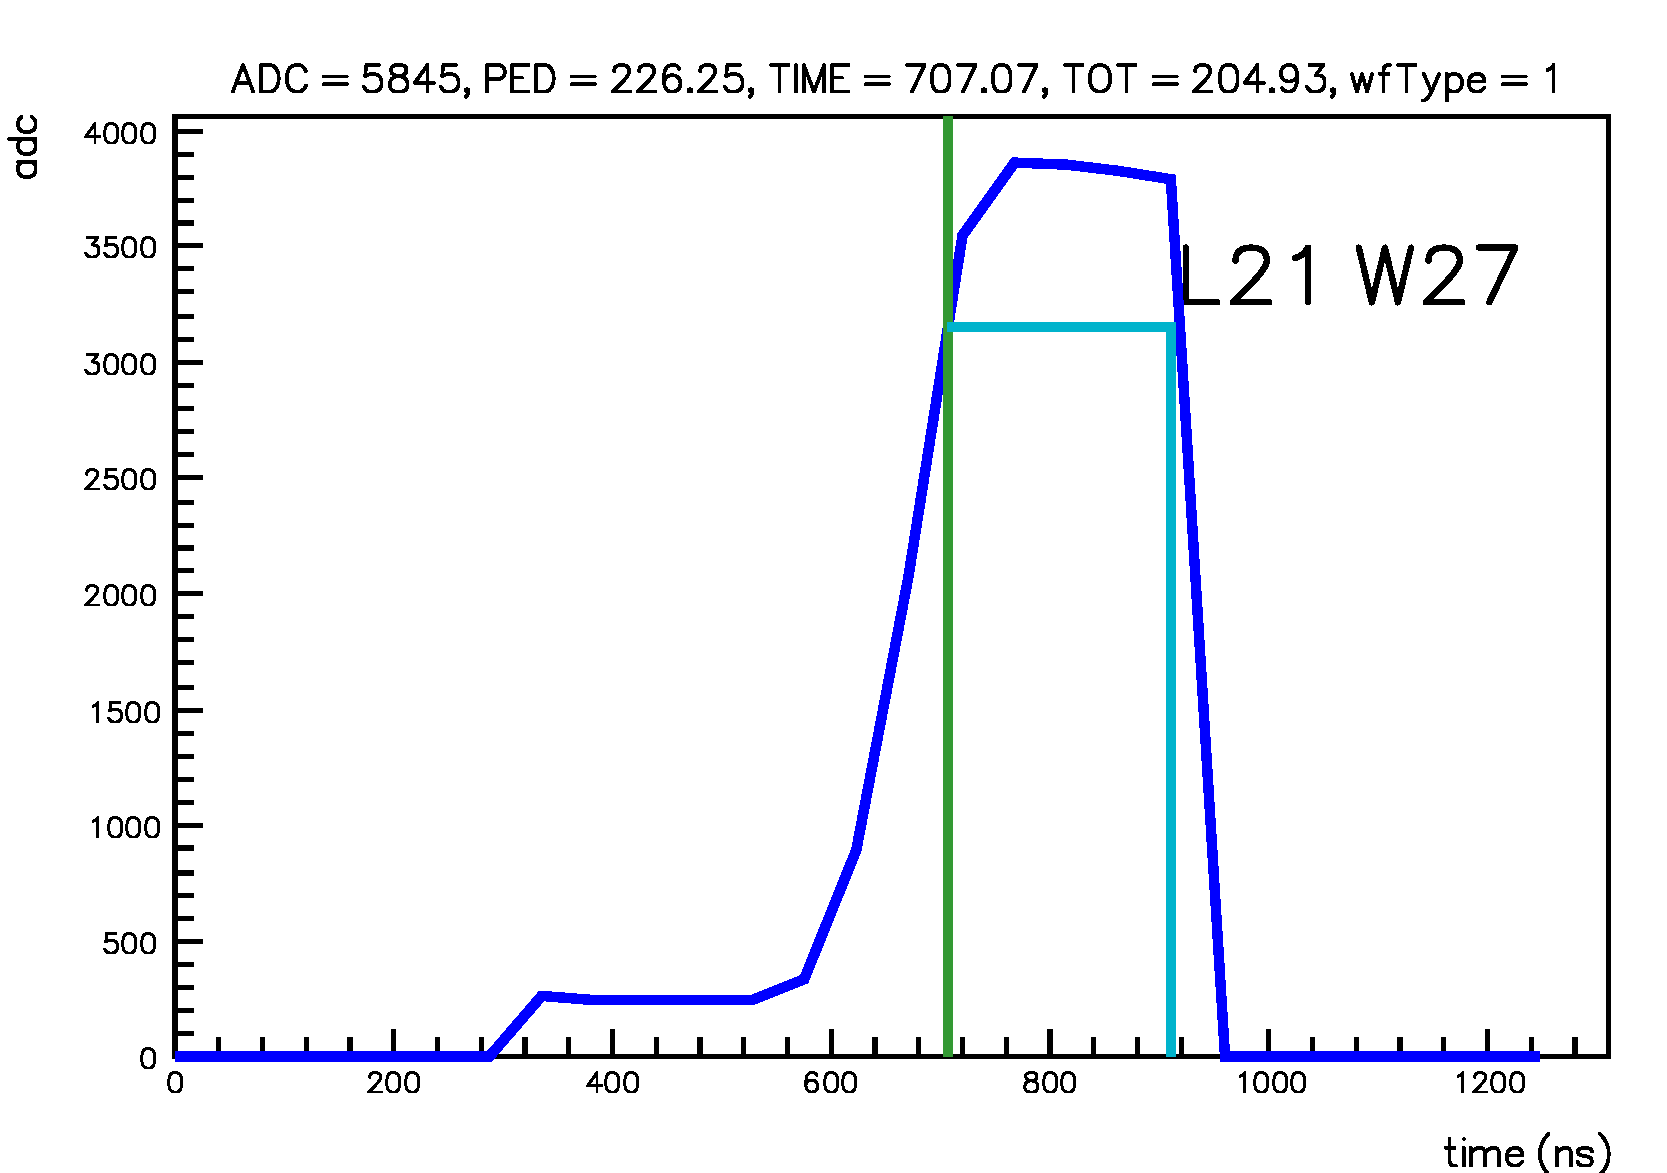
\includegraphics[width=0.45\textwidth]{figures/issue_with_helium_run_num_1_wf2.pdf} \\
            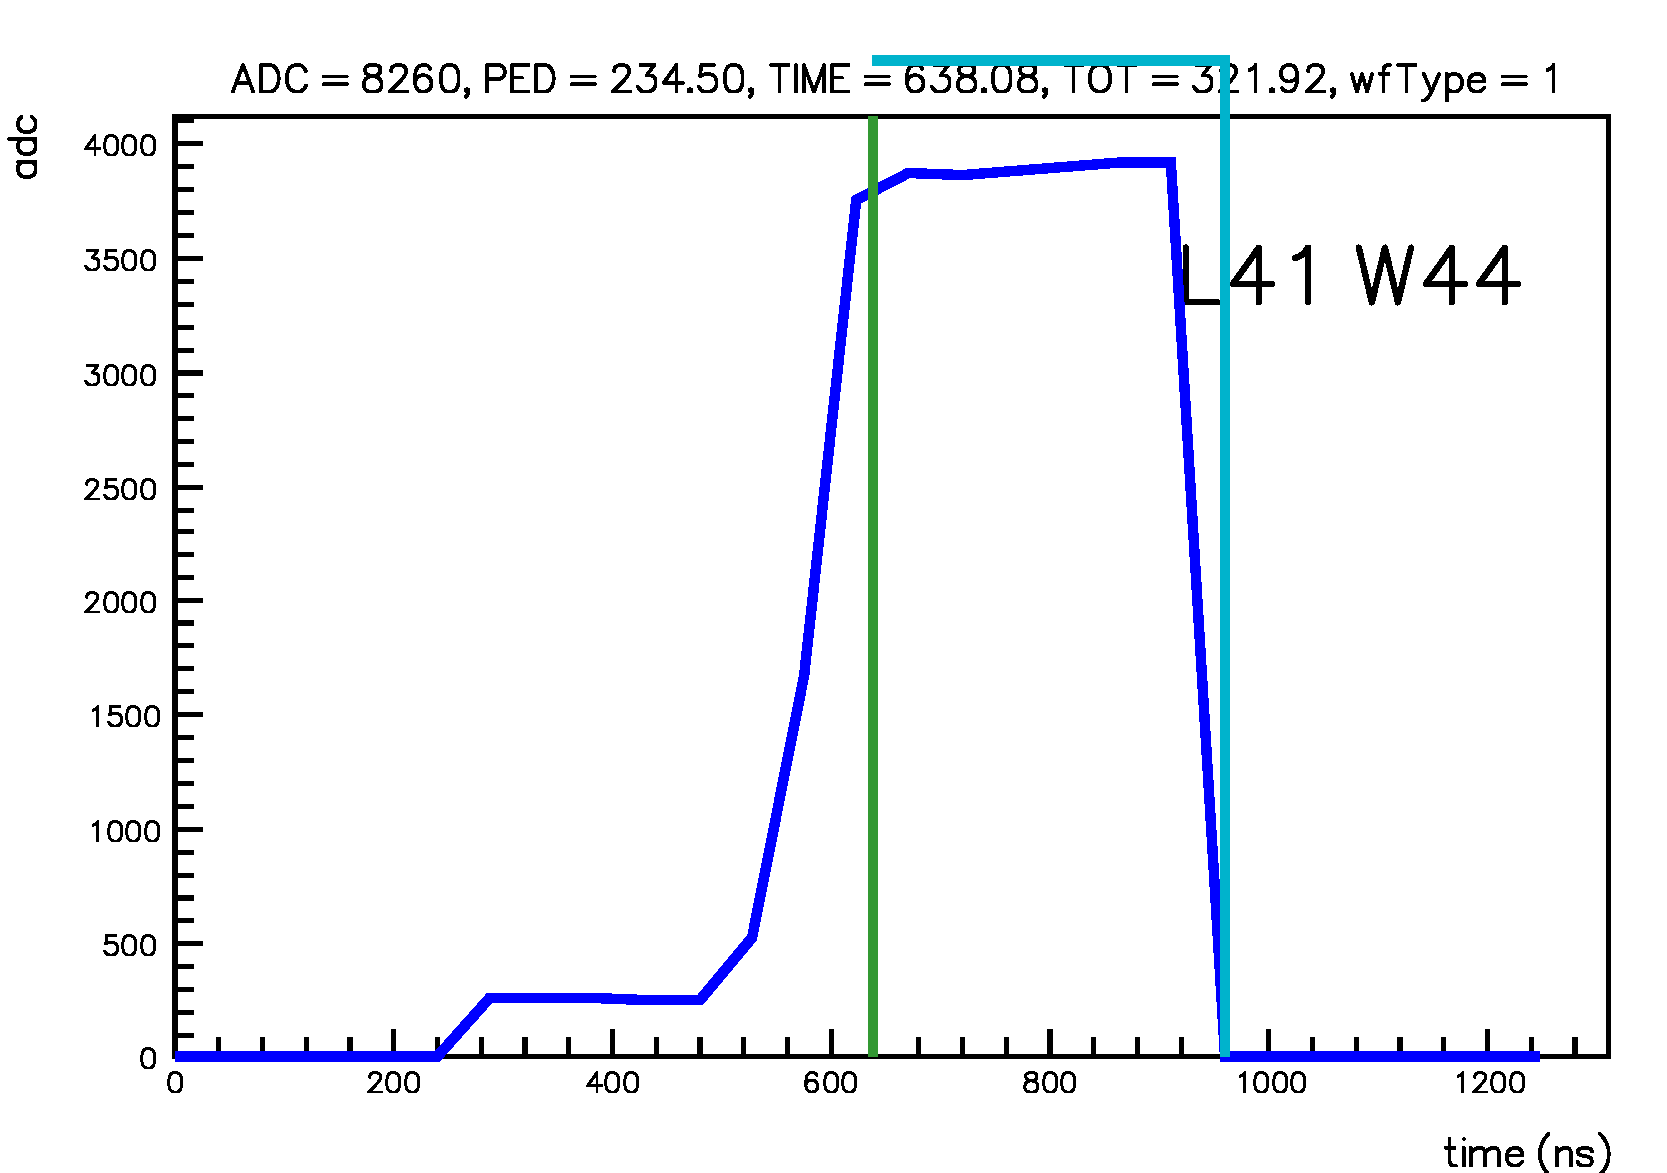
\includegraphics[width=0.45\textwidth]{figures/issue_with_helium_run_num_1_wf3.pdf} &
                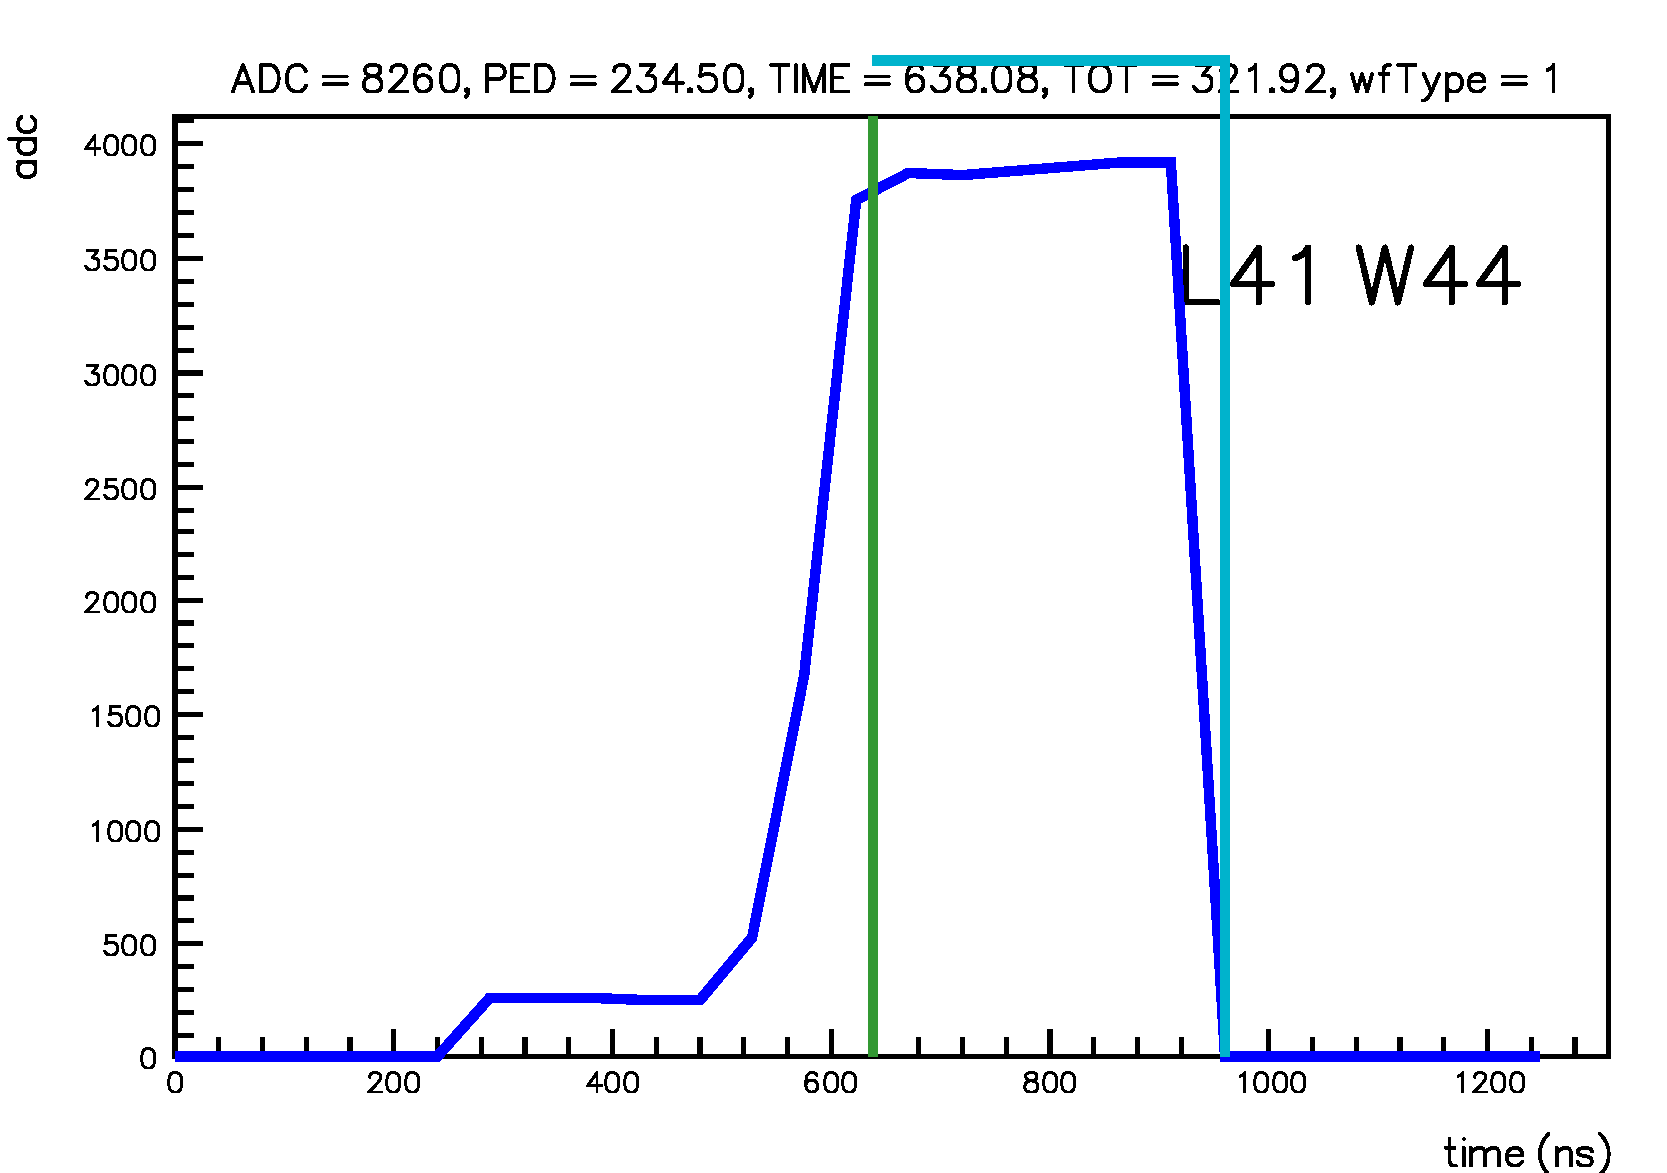
\includegraphics[width=0.45\textwidth]{figures/issue_with_helium_run_num_1_wf3.pdf} \\
        \end{tabular}
    \end{minipage}
    
\end{frame}

\begin{frame}{Track reconstructed in 10.6 GeV data 2/3}
    \begin{itemize}
        \item Left, the reconstructed track is not an artifact, but we do not reconstruct the track with the high deposited energy (as before, excluded due to ToT lower that 300 ns)
            \begin{itemize}
                \item It seems systematics to all data cooked post p0v11
            \end{itemize}
        \item In p0v10\_3, we sometimes manage to catch the high deposited energy
    \end{itemize}

     \vspace{0.5cm}

    \centering
    
    \begin{tabular}{cc}
        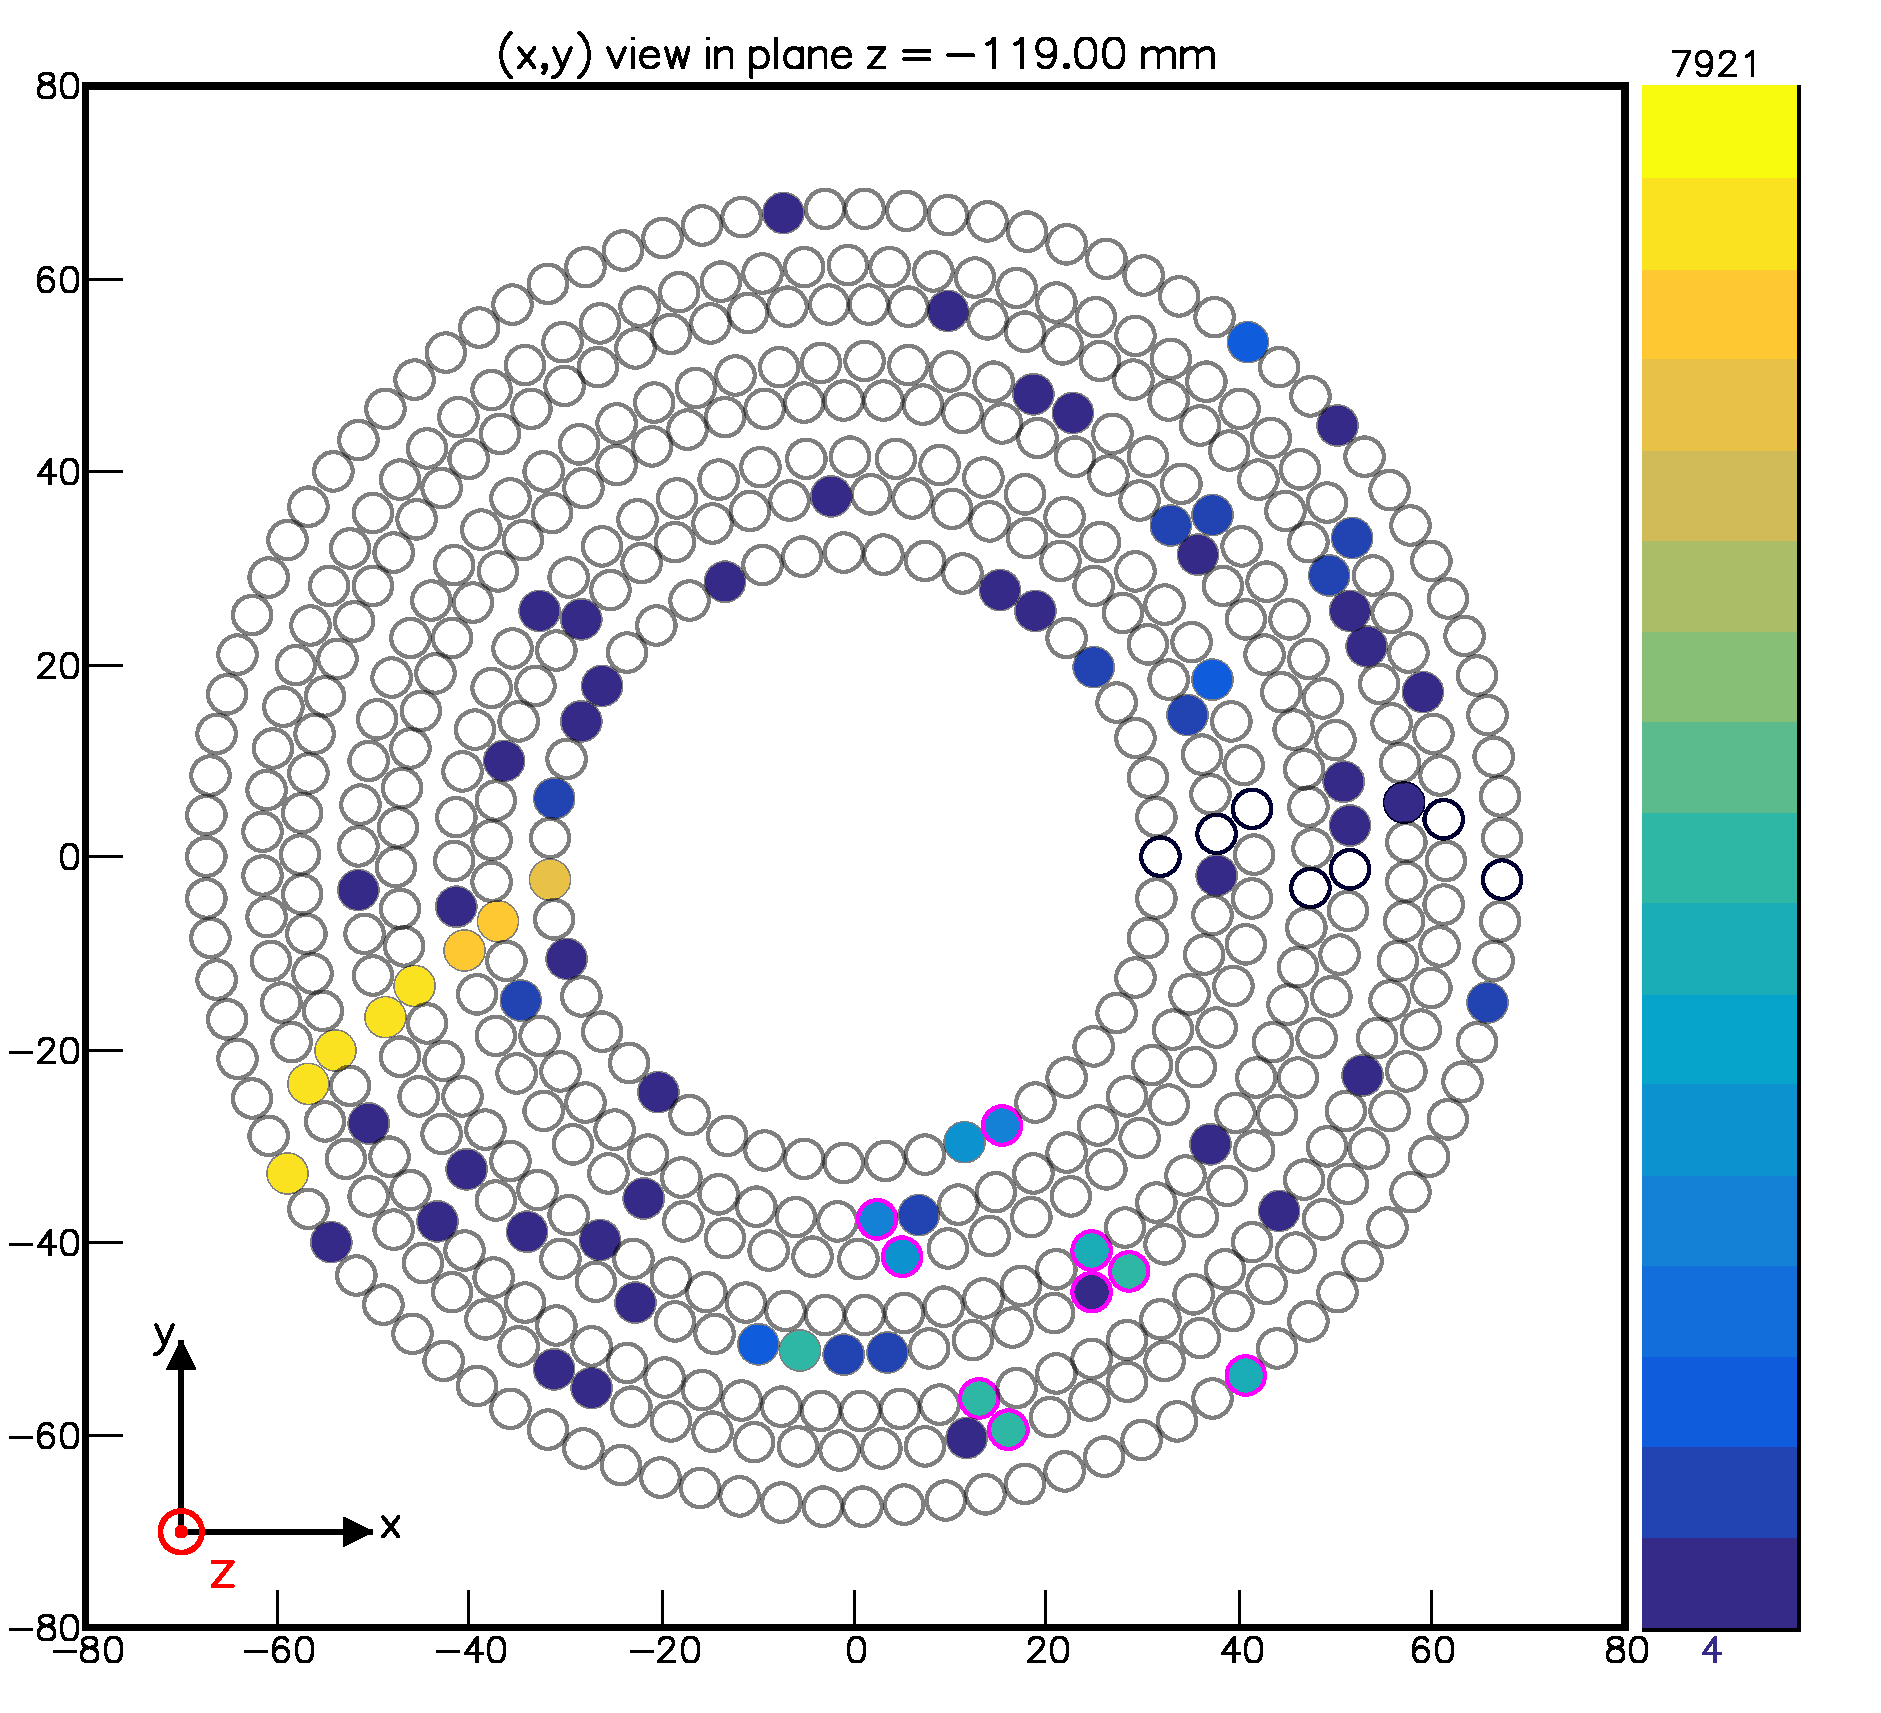
\includegraphics[width=0.45\linewidth]{figures/issue_with_helium_run_num_2.pdf} &
            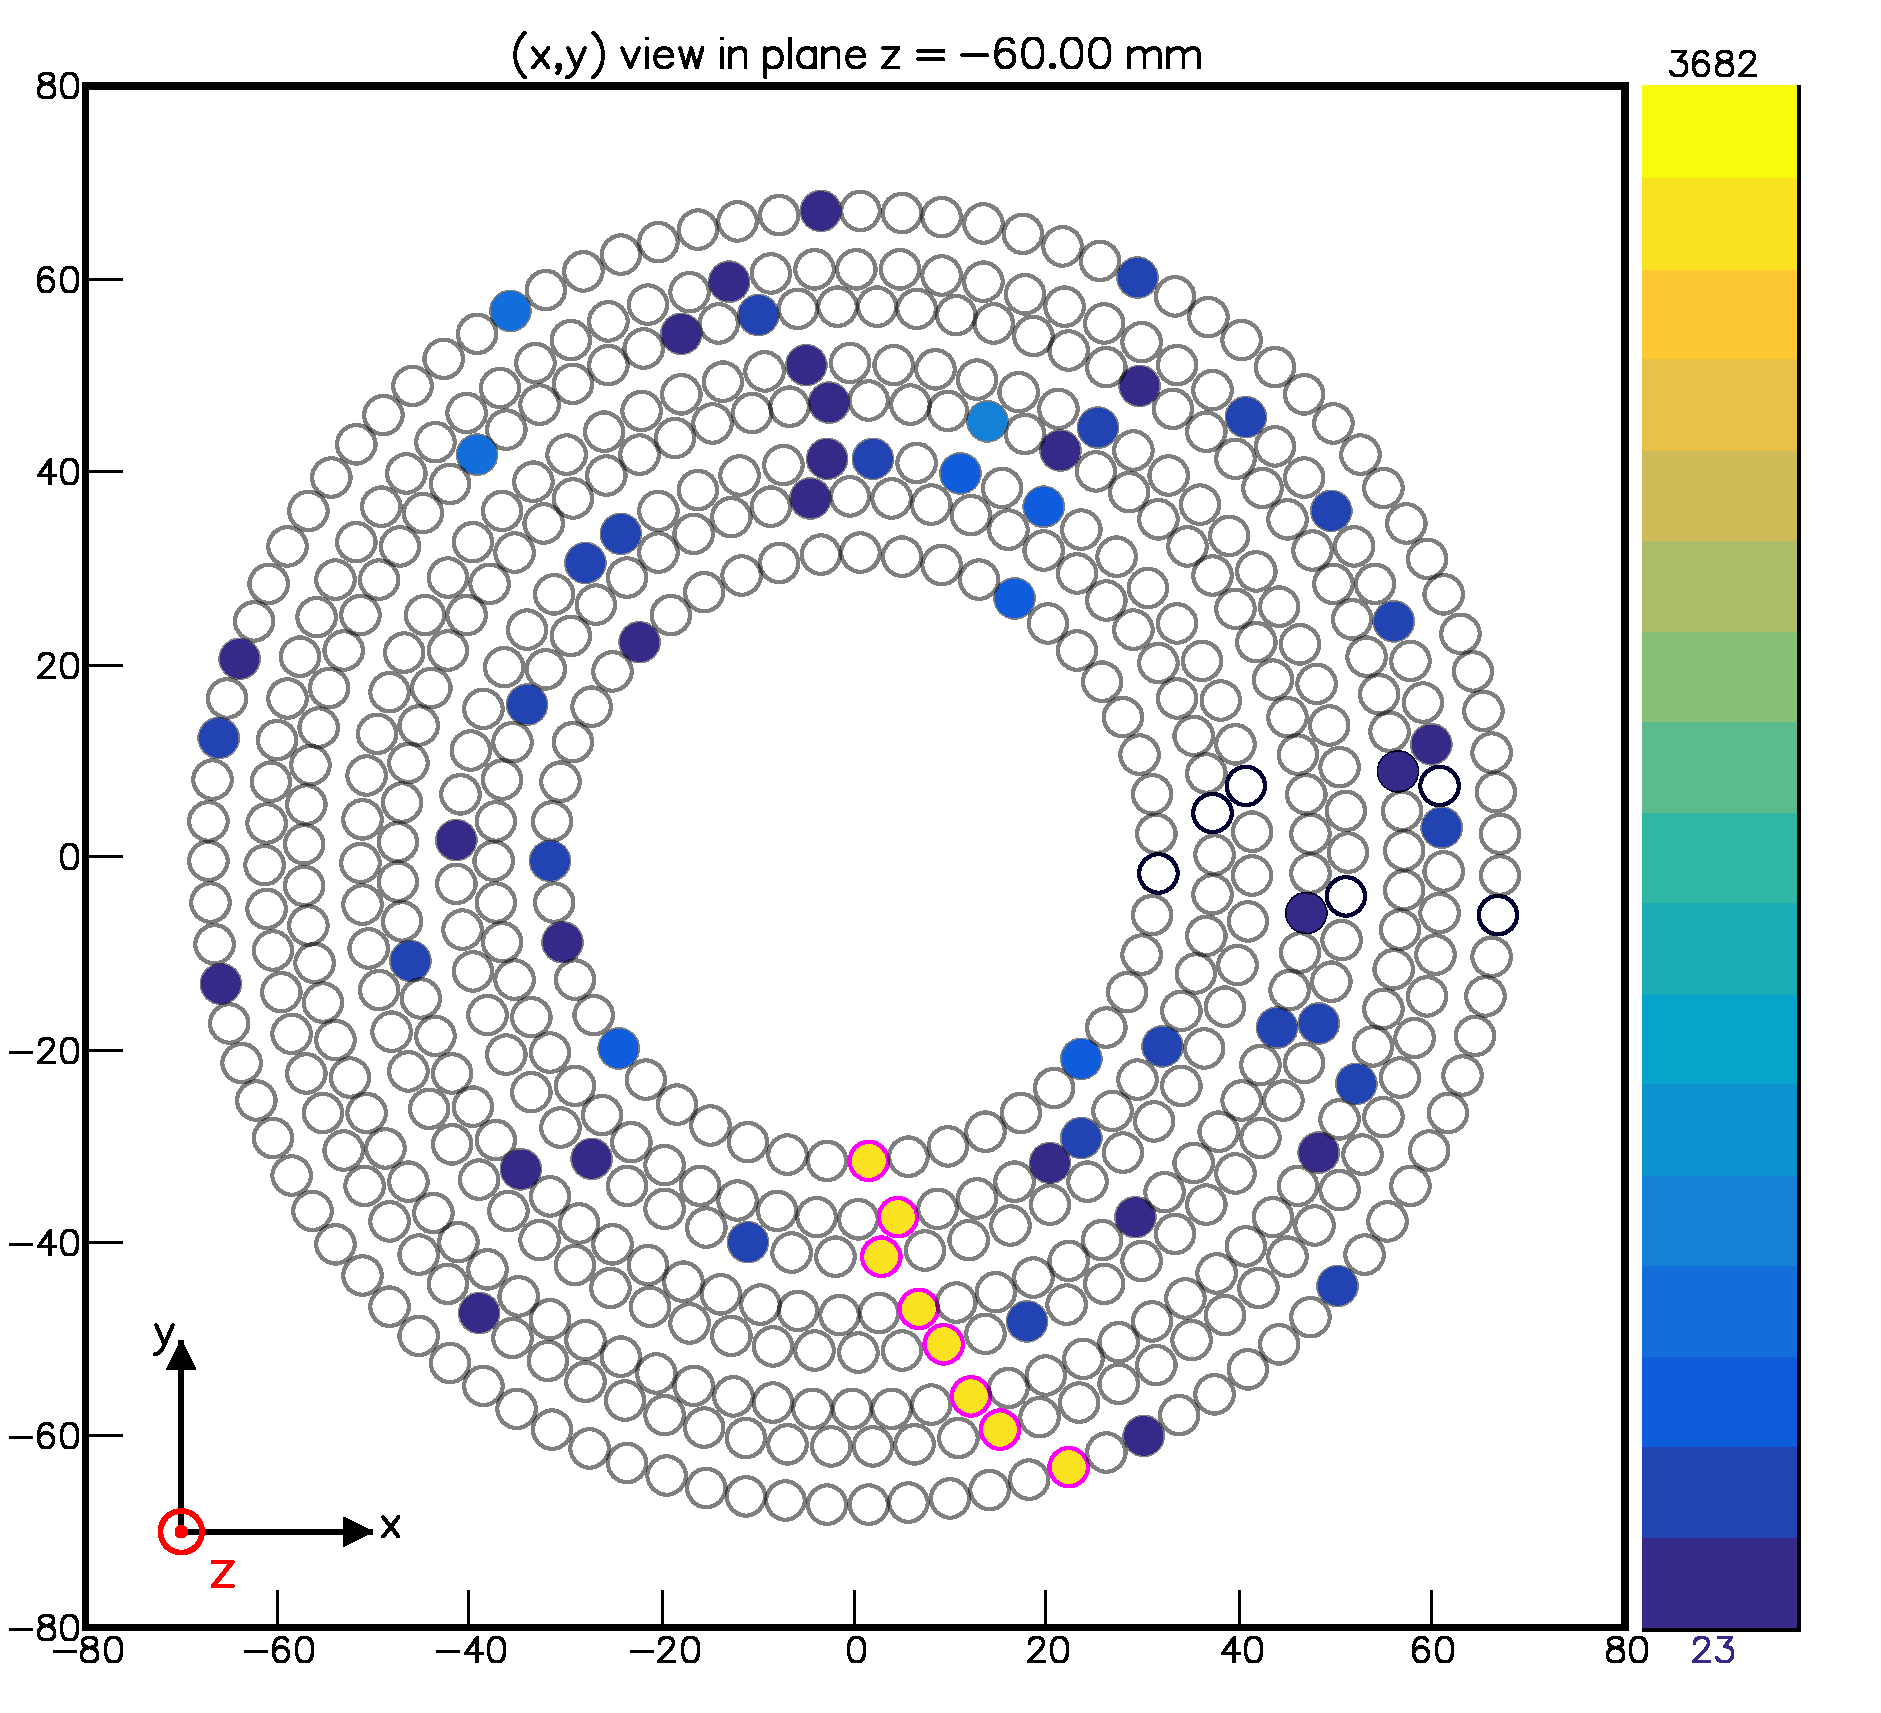
\includegraphics[width=0.45\linewidth]{figures/issue_with_helium_run_num_3_actually_good_in_p0v10_3.pdf} \\
        p0v12 & p0v10\_3
    \end{tabular}
\end{frame}

\begin{frame}{Track reconstructed in 10.6 GeV data 3/3}
    \begin{itemize}
        \item I have added some bias in p0v12, but even in p0v10\_3, we miss potential good tracks
            \begin{itemize}
                \item Here, the ToT were in the good interval
                \item A possible reason is that their time reconstruction was not good enough (again, the time should be better in p0v12, but we still have a ToT cut that makes no sense)
            \end{itemize}
    \end{itemize}

     \vspace{0.5cm}

    \centering
    
    \begin{tabular}{cc}
        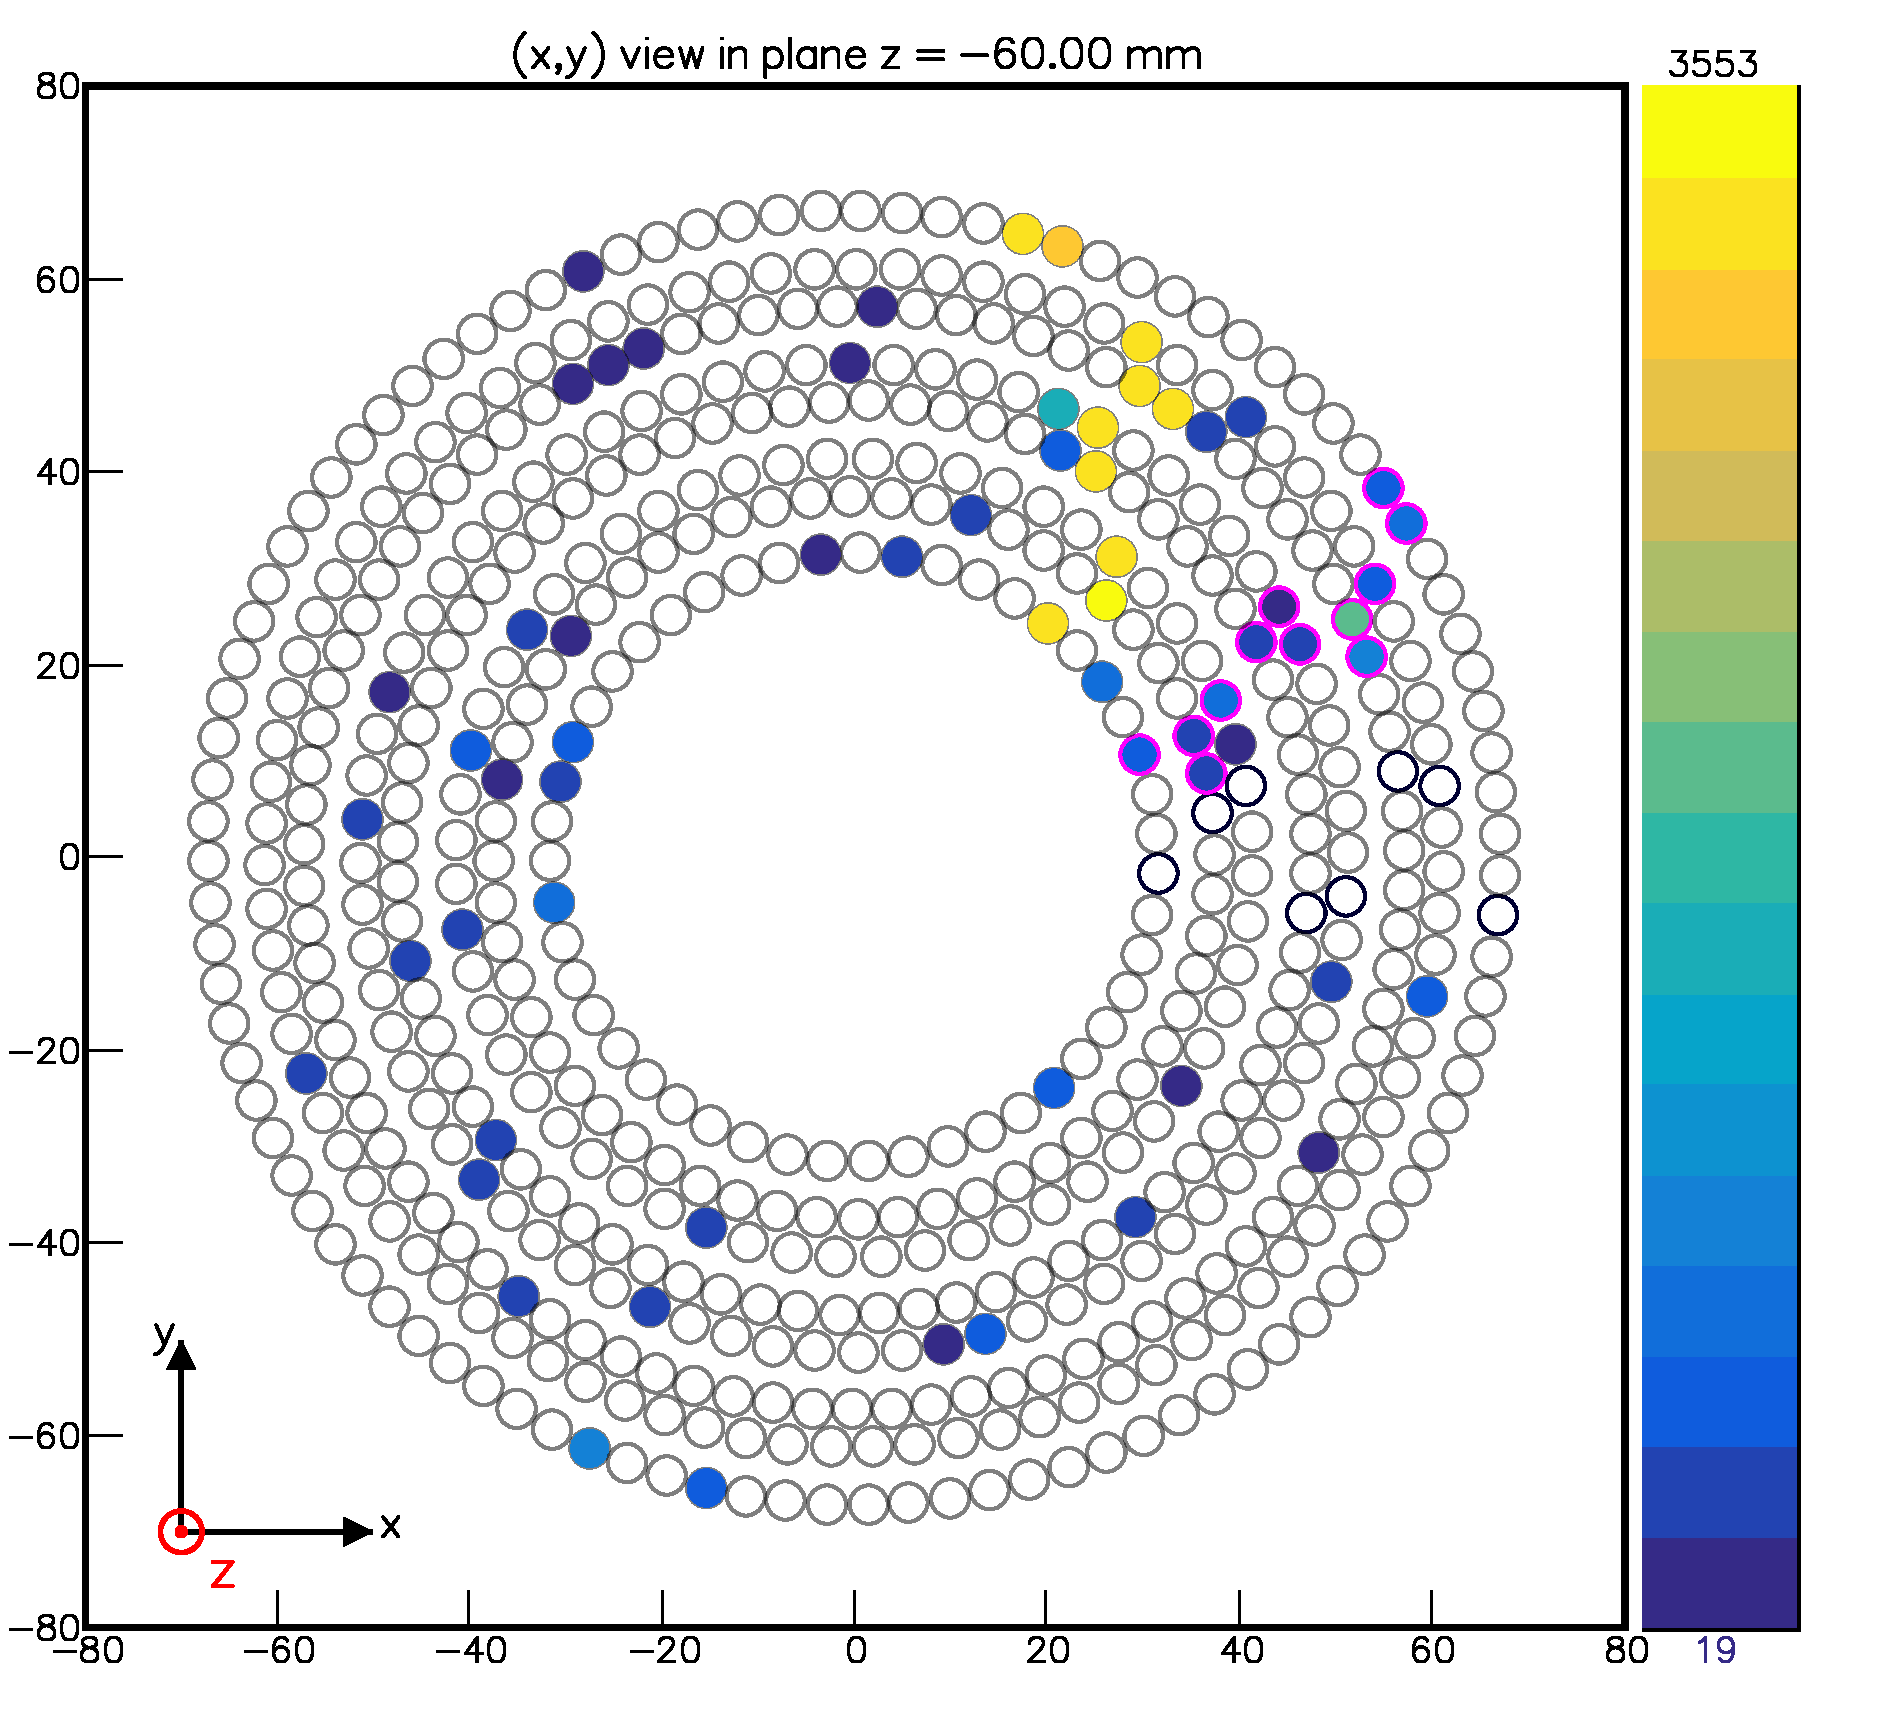
\includegraphics[width=0.45\linewidth]{figures/issue_with_helium_run_num_4_p0v10_3.pdf} &
            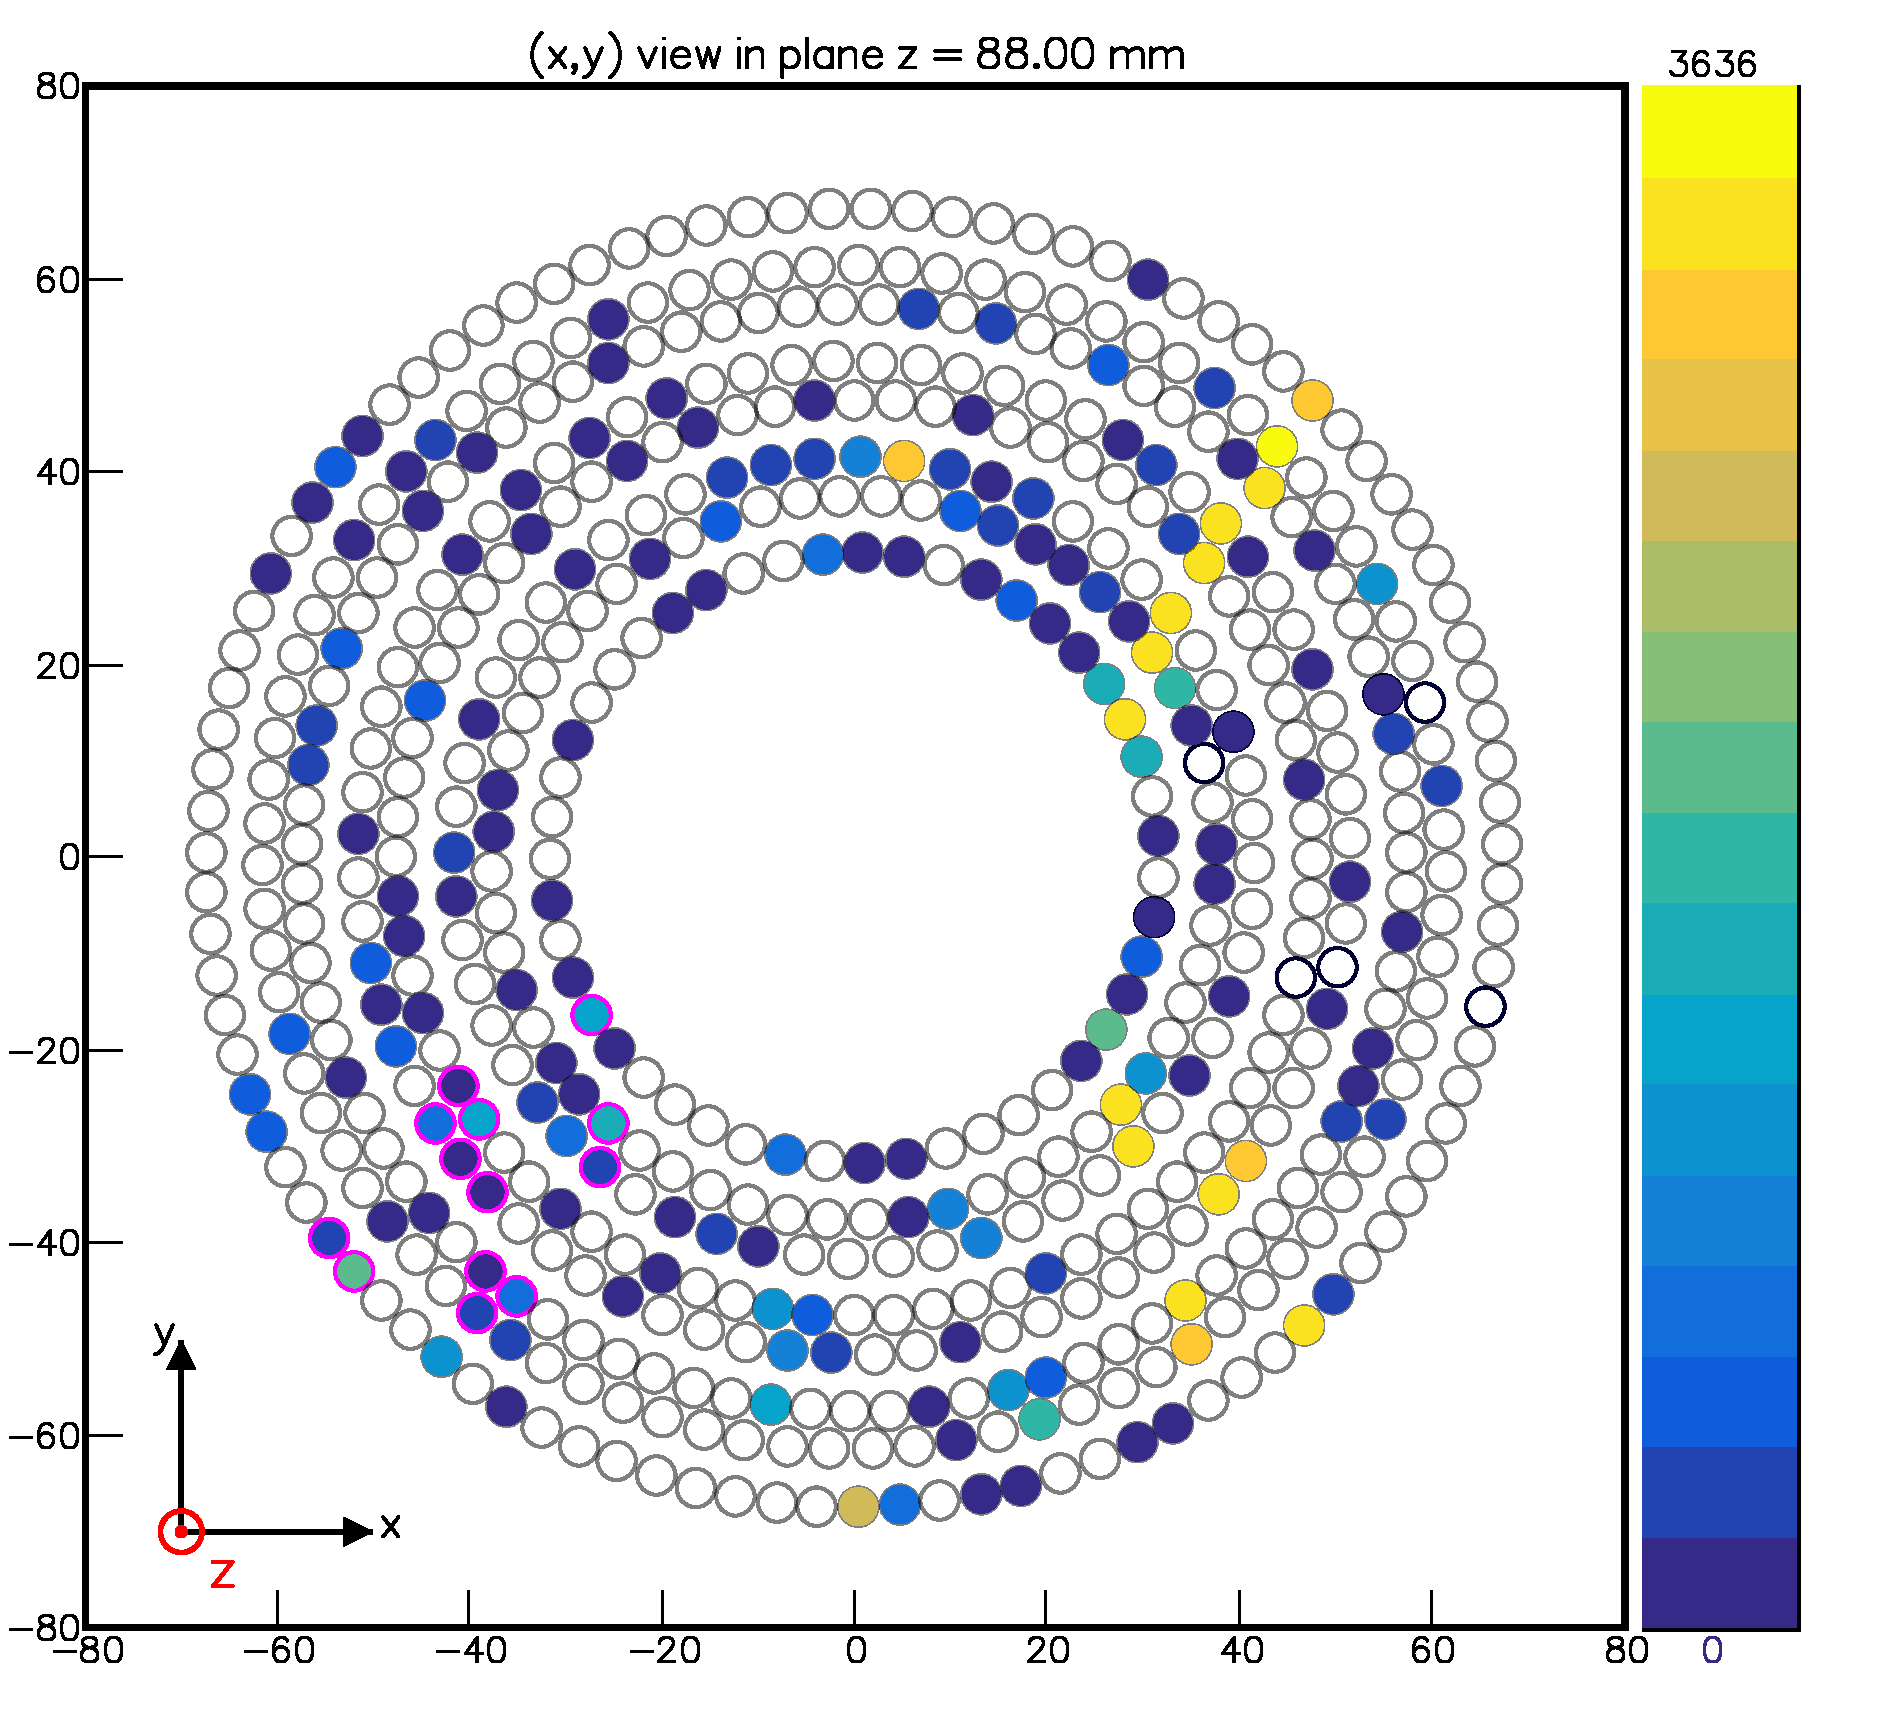
\includegraphics[width=0.45\linewidth]{figures/issue_with_helium_run_num_5_p0v10_3.pdf}
    \end{tabular}
\end{frame}

\begin{frame}{Conclusion}
    \begin{itemize}
        \item The track reconstruction is well controlled at 2.24 GeV and low beam intensity
            \begin{itemize}
                \item Track hits are easily selected
                \item The issue encountered can be easily fixed by removing the pedestal and updating the ToT threshold
            \end{itemize}
        \item The track reconstruction for 10.6 GeV run is difficult
            \begin{itemize}
                \item The hit selection should be revisited
                \item The t0 and T2D should be provided
                \item We still reconstruct tracks, but some of them are artifacts
                \item I plan to investigate those events by looking at elastic events off 4He
            \end{itemize}
    \end{itemize}
\end{frame}


\begin{frame}{Appendix - Zero suppression}
    \centering
    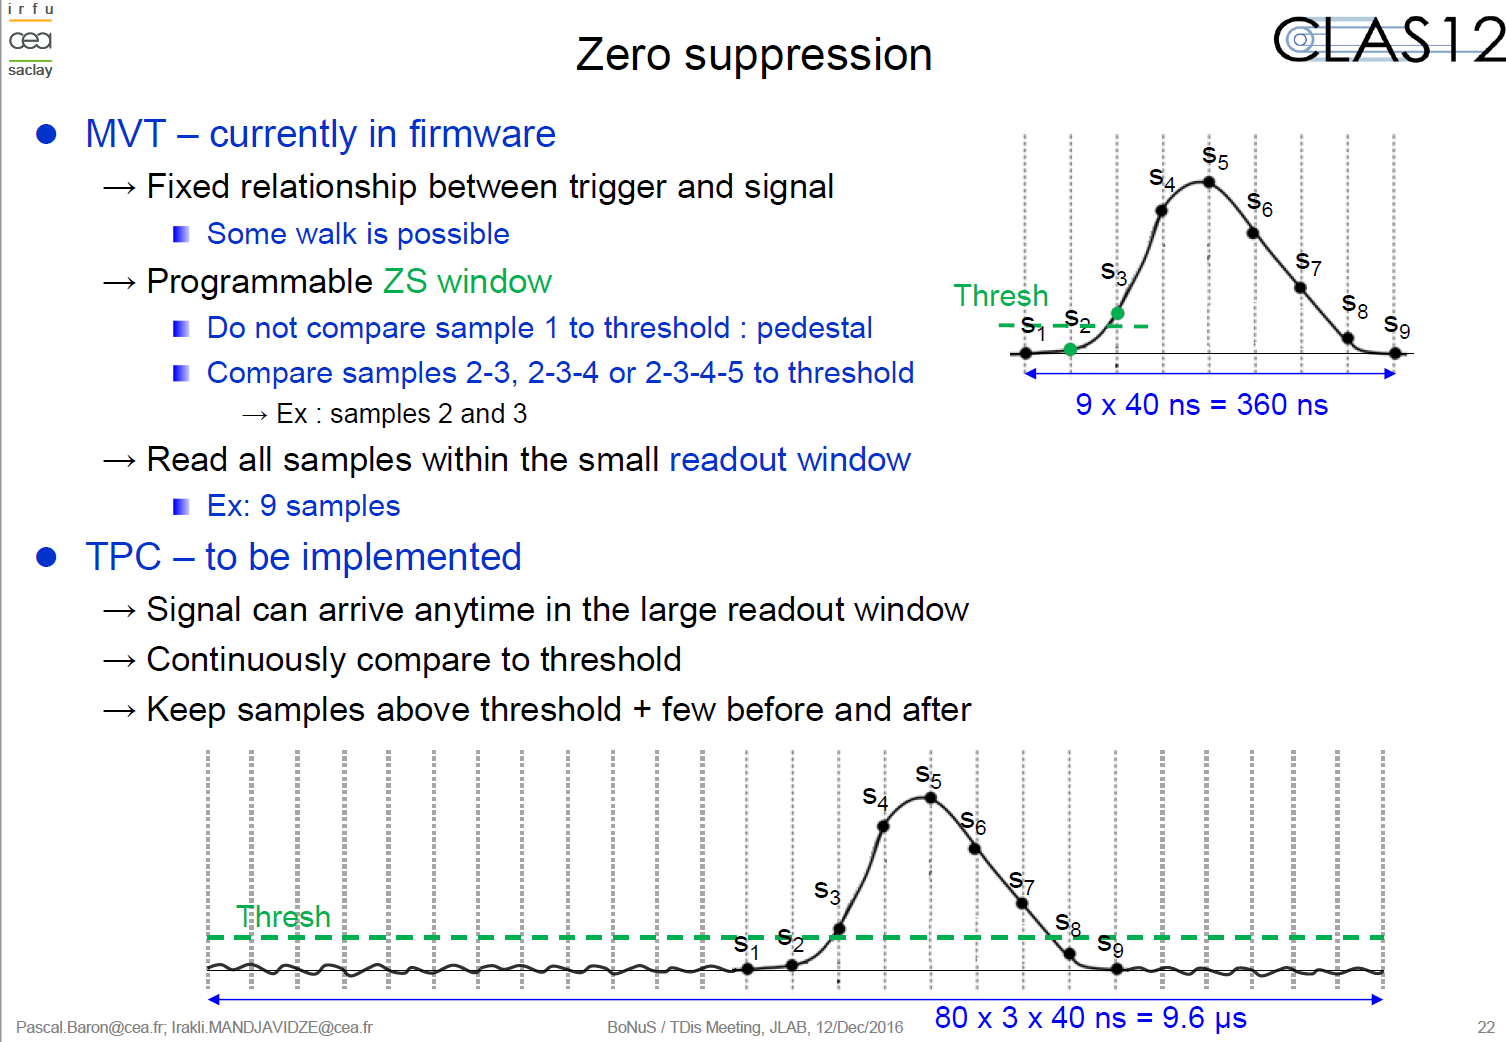
\includegraphics[width=0.9\linewidth]{figures/TrakerVsTPC_ZS.png}
\end{frame}

















\end{document}


